%%%%%%%%%%%%%%%%%%%%%%%%%%%%%%%%%%%%%%%%%
% Journal Article
% LaTeX Template

\documentclass{article}

\usepackage{hyperref}
\usepackage[sc]{mathpazo} % Use the Palatino font
\usepackage[T1]{fontenc} % Use 8-bit encoding that has 256 glyphs
\linespread{1.3} % Line spacing - Palatino needs more space between lines
\usepackage{microtype} % Slightly tweak font spacing for aesthetics
\usepackage{listings}   % Include the listings-package
\usepackage[hmarginratio=1:1,top=32mm,columnsep=20pt]{geometry} % Document margins
\usepackage{multicol} % Used for the two-column layout of the document
\usepackage[hang, small,labelfont=bf,up,textfont=it,up]{caption} % Custom captions under/above floats in tables or figures
\usepackage{booktabs} % Horizontal rules in tables
\usepackage{float} % Required for tables and figures in the multi-column environment - they need to be placed in specific locations with the [H] (e.g. \begin{table}[H])
\usepackage{hyperref} % For hyperlinks in the PDF
\usepackage{graphicx}
\usepackage{pdfpages}
\graphicspath{.}
\usepackage{abstract} % Allows abstract customization
\usepackage{amsmath}
\renewcommand{\abstractnamefont}{\normalfont\bfseries} % Set the "Abstract" text to bold
\renewcommand{\abstracttextfont}{\normalfont\small\itshape} % Set the abstract itself to small italic text
\usepackage{multirow}
\usepackage{titlesec} % Allows customization of titles

\usepackage{fancyhdr} % Headers and footers
\pagestyle{fancy} % All pages have headers and footers
\fancyhead{} % Blank out the default header
\fancyfoot{} % Blank out the default footer
\fancyhead[C]{BINP25 project $\bullet$ October 2016 } % Custom header text
\fancyfoot[RO,LE]{\thepage} % Custom footer text
\usepackage{amsmath}
%----------------------------------------------------------------------------------------
%	TITLE SECTION
%----------------------------------------------------------------------------------------

\title{\vspace{1mm}\fontsize{16pt}{12pt}\selectfont\textbf{Analysis of tri-axial accelerometer data of 4 month old infants}} % Article title

\author{
\large
\text{Student:}
\textsc{Jerneja Mislej}\\[2mm] % Your name
\normalsize University of Lund \\ % Your institution
\normalsize \href{mailto:bif15jmi@student.lu.se}{bif15jmi@student.lu.se}\\\\ % Your email address
\large
\text{Project supervisor:}
\textsc{Frida Renstrom}\\[2mm] % Your name
\normalsize University of Lund \\ % Your institution
\normalsize \href{mailto:Frida.Renstrom@med.lu.se}{Frida.Renstrom@med.lu.se}\\ % Your email address
\large \\
\text{Assistant project supervisors:}
\textsc{Paul W. Franks, Azra Kurbasic}\\[2mm] % Your name
\normalsize University of Lund \\ % Your institution
\normalsize \href{mailto:Paul.Franks@med.lu.se}{Paul.Franks@med.lu.se}\\ \\% Your email address
\normalsize \href{mailto:Azra.Kurbasic@med.lu.se}{Azra.Kurbasic@med.lu.se}\\
\vspace{-5mm}
}
\date{}


%----------------------------------------------------------------------------------------

\begin{document}

\maketitle % Insert title

\thispagestyle{fancy} % All pages have headers and footers

%---------------------------------ph-------------------------------------------------------
%	ABSTRACT
%----------------------------------------------------------------------------------------

\begin{abstract}

\noindent 
\fontsize{10pt}{11pt}\selectfont {The main goal of the project is to extract a measure of physical activity levels from tri-axial accelerometer data, taken of four month old infants and to assess the feasibility and validation of the extraction. 30 infants wore two accelerometers, one on the torso, other on the ankle, for 48 hours in a free living environment. In order to properly extract physical activity level data, the raw accelerometer output has to be prepared and preprocessed. Preparation includes data organization and time-stamp alignment, while the preprocessing includes filtering, averaging, removal of non-wear time, summary measure derivation, correction for gravity component and correction for acceleration contributed by the infants caretaker. Several approaches are used and the performance of each discussed. The results from the correction of caretakers contributing accelerations are compared against the diary notations of the infants sleeping and feeding habits, kept by their mothers. In the end, physical activity levels are extracted and analyzed, focusing on the assessment of the feasibility and validation of the extraction. 
\\\\}

\end{abstract}
\tableofcontents{}
\newpage
%----------------------------------------------------------------------------------------
%	ARTICLE CONTENTS
%----------------------------------------------------------------------------------------

\section{Introduction}

\fontsize{11.25pt}{11.1pt}\selectfont {The tri-axial accelerometer data was obtained in the Energy balance and health in pregnancy study, a pre-pilot study for LifeGene (http://www.lifegene.se). One of the aims of the pre-pilot study was to assess the feasibility of estimating physical activity (PA) in young infants in order to associate lifestyle behaviors during pregnancy and post-partum markers of infant cardiometabolic health. An extensive collection of characteristics was measured and obtained, including infant and maternal tri-axial accelerometer data and infant sleeping and feeding diaries. Mothers characteristics in pregnancy, along with the infants characteristics post-partum, can provide valuable information when studying fetal programming\cite{ref14}\cite{ref15}\cite{ref16}. Infants at 4 months post-partum will not yet have been substantially exposed to and influenced by the environment outside the intrauterine environment, especially when it comes to PA, which is consequently more instinct at that point and can therefor be considered pre-programmed. By being able to accurately estimate infants PA, many research questions could be addressed.\\\\
In this project, estimation of infant PA is addressed along with an assessment of the feasibility regarding such an estimation.
Although accelerometers are increasingly being used for PA estimations in population studies, their output needs to be interpreted with caution. Due to its properties and sensitivity, the accelerometer is prone to pick up accelerations not related to the PA of the subject wearing it. In measurements taken of adults, these are mainly due to gravitation and instrumentation noise, but in infants and smaller children who are less or not mobile in terms of walking, the caretaker contributes greatly to the acceleration by carrying or placing the child \cite{ref1}. By not appropriately considering acceleration contributed by the caretaker, the extracted infant PA would incorrectly present infants that are moved around more as being more active.\\\\
For that purpose, the pre-pilot project was designed to place two accelerometers on the infant, one on the torso, other on the ankle. The rationale behind this was that infants at four months of age are unable to move the torso by themselves, so any large accelerations measured on the torso would consequently mean that the infant was being moved. On the other hand, the infant can move his legs, so having accelerations detected on the ankle accelerometer, but not on the torso, would mean the infant is being active by own account. At the same time, the mothers, who were the main caretakers of the infants in the present study, also wore a wrist accelerometer and kept a diary of feeding and sleeping habits of the infant, as well as other important information concerning the infant and the experiment.

}

%------------------------------------------------

\section{Methods}

\fontsize{11.25pt}{11.1pt}\selectfont {
Acceleration data was recorded on 30 mother and infant pairs, in a free living environment, for 48 hours, using a tri-axial GENEA accelerometer (UniLever Ltd), sampled at 40 Hz and stored in g units. In order to properly analyze the tri-axial accelerometer data, preparation and preprocessing of the data needs to be performed. As the infant torso, infant ankle and maternal accelerometers did not start measuring at the exact same time, the measurements need to be aligned according to timestamps, to ensure they represent accelerations recorded at the same time.
This is followed by accelerometer non-wear data removal, summary measure derivation and correction for the gravitational acceleration.
In the last step of preprocessing, the contributing accelerations need to be addressed even further. Generally, accelerometers will record any movement, regardless whether the movement is due to PA of the subject wearing it or due to the subject being moved or carried, or even due to just readjustment of the accelerometer. The accelerometer data needs to be cleaned, so that the remaining accelerations are due to infants PA only. If the preprocessing and data cleaning is efficient, then infants PA can simply be extracted based on appropriate cut points for the standard deviation of the acceleration.

\subsection{Time-stamp alignment}
The accelerometers were attached upon a visit to the research clinic. With few exceptions, accelerometers were set to start recording before being attached and were attached to the mothers wrist, infants torso and infants ankle one after the other. This resulted in different start timestamps. In order to ensure proper analysis of the data, the measurements needed to be aligned so that for each mother-infant pair, all three measurements had the same start time-stamp.
The alignment is done with a Python script that loaded and read all three files belonging to the measurements of each mother-infant pair, processed the data and saved the results. Files are loaded using the module \textit{pandas}. The timestamps of the accelerometer are in the YYYY-MM-DD HH:MM:SS:ffff format and are parsed with the module \textit{dateutil} which enables the resulting parsed timestamps to be simply compared with each other. The latest start time-stamp is determined and converted back into the appropriate format with \textit{strftime} from the \textit{os} module. This time-stamp is then located in the rest of the measurements which are truncated up to that index. The resulting three measurements are aligned according to the absolute time-stamp and are saved, again using the module \textit{pandas}. 

\subsection{Accelerometer non-wear time}
With exception of the accelerometer placed on the infants ankle, the accelerometers could be removed and reattached. Mothers were asked to note such non-wear time in the diary. Prior to diary examination, non-wear time is detected automatically with a Python script. The diary notations are then used for validation of the results. The Python script is designed based on previous approaches towards non-wear time removal \cite{ref2}. The principal idea of the approach is to examine the standard deviation (SD) and the span between minimum and maximum of a windowed measurement and remove windows where the SD and span are below certain cut points defined in published methods \cite{ref2}. To increase accuracy, the baseline of the windowed measurement is also examined in this project. When the accelerometer is not worn by the subject, it should only be picking up acceleration due to gravitation which is constant on one axis only. As a consequence, the measurement of non-wear time should in theory have none or very little SD, the span between the minimum value and the maximum value should be close to zero and the baseline of the measurement should be a flat line without any drift or jumps.\\In practice, one cannot fully rely on these assumptions. All accelerometers have inherent noise, for the accelerometer used in the current project (GENEA), it has been shown that the SD of a motionless device is 2.6 mg. Other factors can also contribute towards the increased SD, since being in a free living environment, the accelerometer is liable to pick up the movement from the environment, even if only the surface on which it rests is being bumped into. On the other hand, if the accelerometer is not placed on the torso, it will not pick up accelerations due to heartbeats and chest movements from breathing\cite{ref8}, and can therefore appear as non-wear time when the subject is actually sleeping very still. All this has to be taken into consideration when extracting and removing the data of non-wear time and several parameters need to be set which greatly affect the final outcome. For this reason, some parameters are left to be passed on to the script upon run time in order to enable trial and examination. These parameters are: 
\begin{itemize}
\item Window length
\item SD threshold
\item Span between minimum and maximum threshold
\end{itemize}
These parameters are read with the module \textit{sys}. Data is loaded and read with the module \textit{pandas}. Each of the three axis are filtered with a median filter of width 11, using \textit{medfilt} from module \textit{scipy.signal}. The measurement is windowed with a loop. For each window, SD and span between minimum and maximum is calculated. If these values are below the set thresholds, a line is fitted through the accelerometer data points of the window with the help of \textit{polyfit} from the module \textit{numpy}. The slope of the line should be near to zero. The value of \textit{1e-07} is chosen as the threshold and if the absolute value of the slope is below that threshold, the window is classified as non-wear time. The data along with the results are plotted using module \textit{matplotlib} and printed in the terminal, example in Figure 1.
\newpage
\begin{figure}[h]
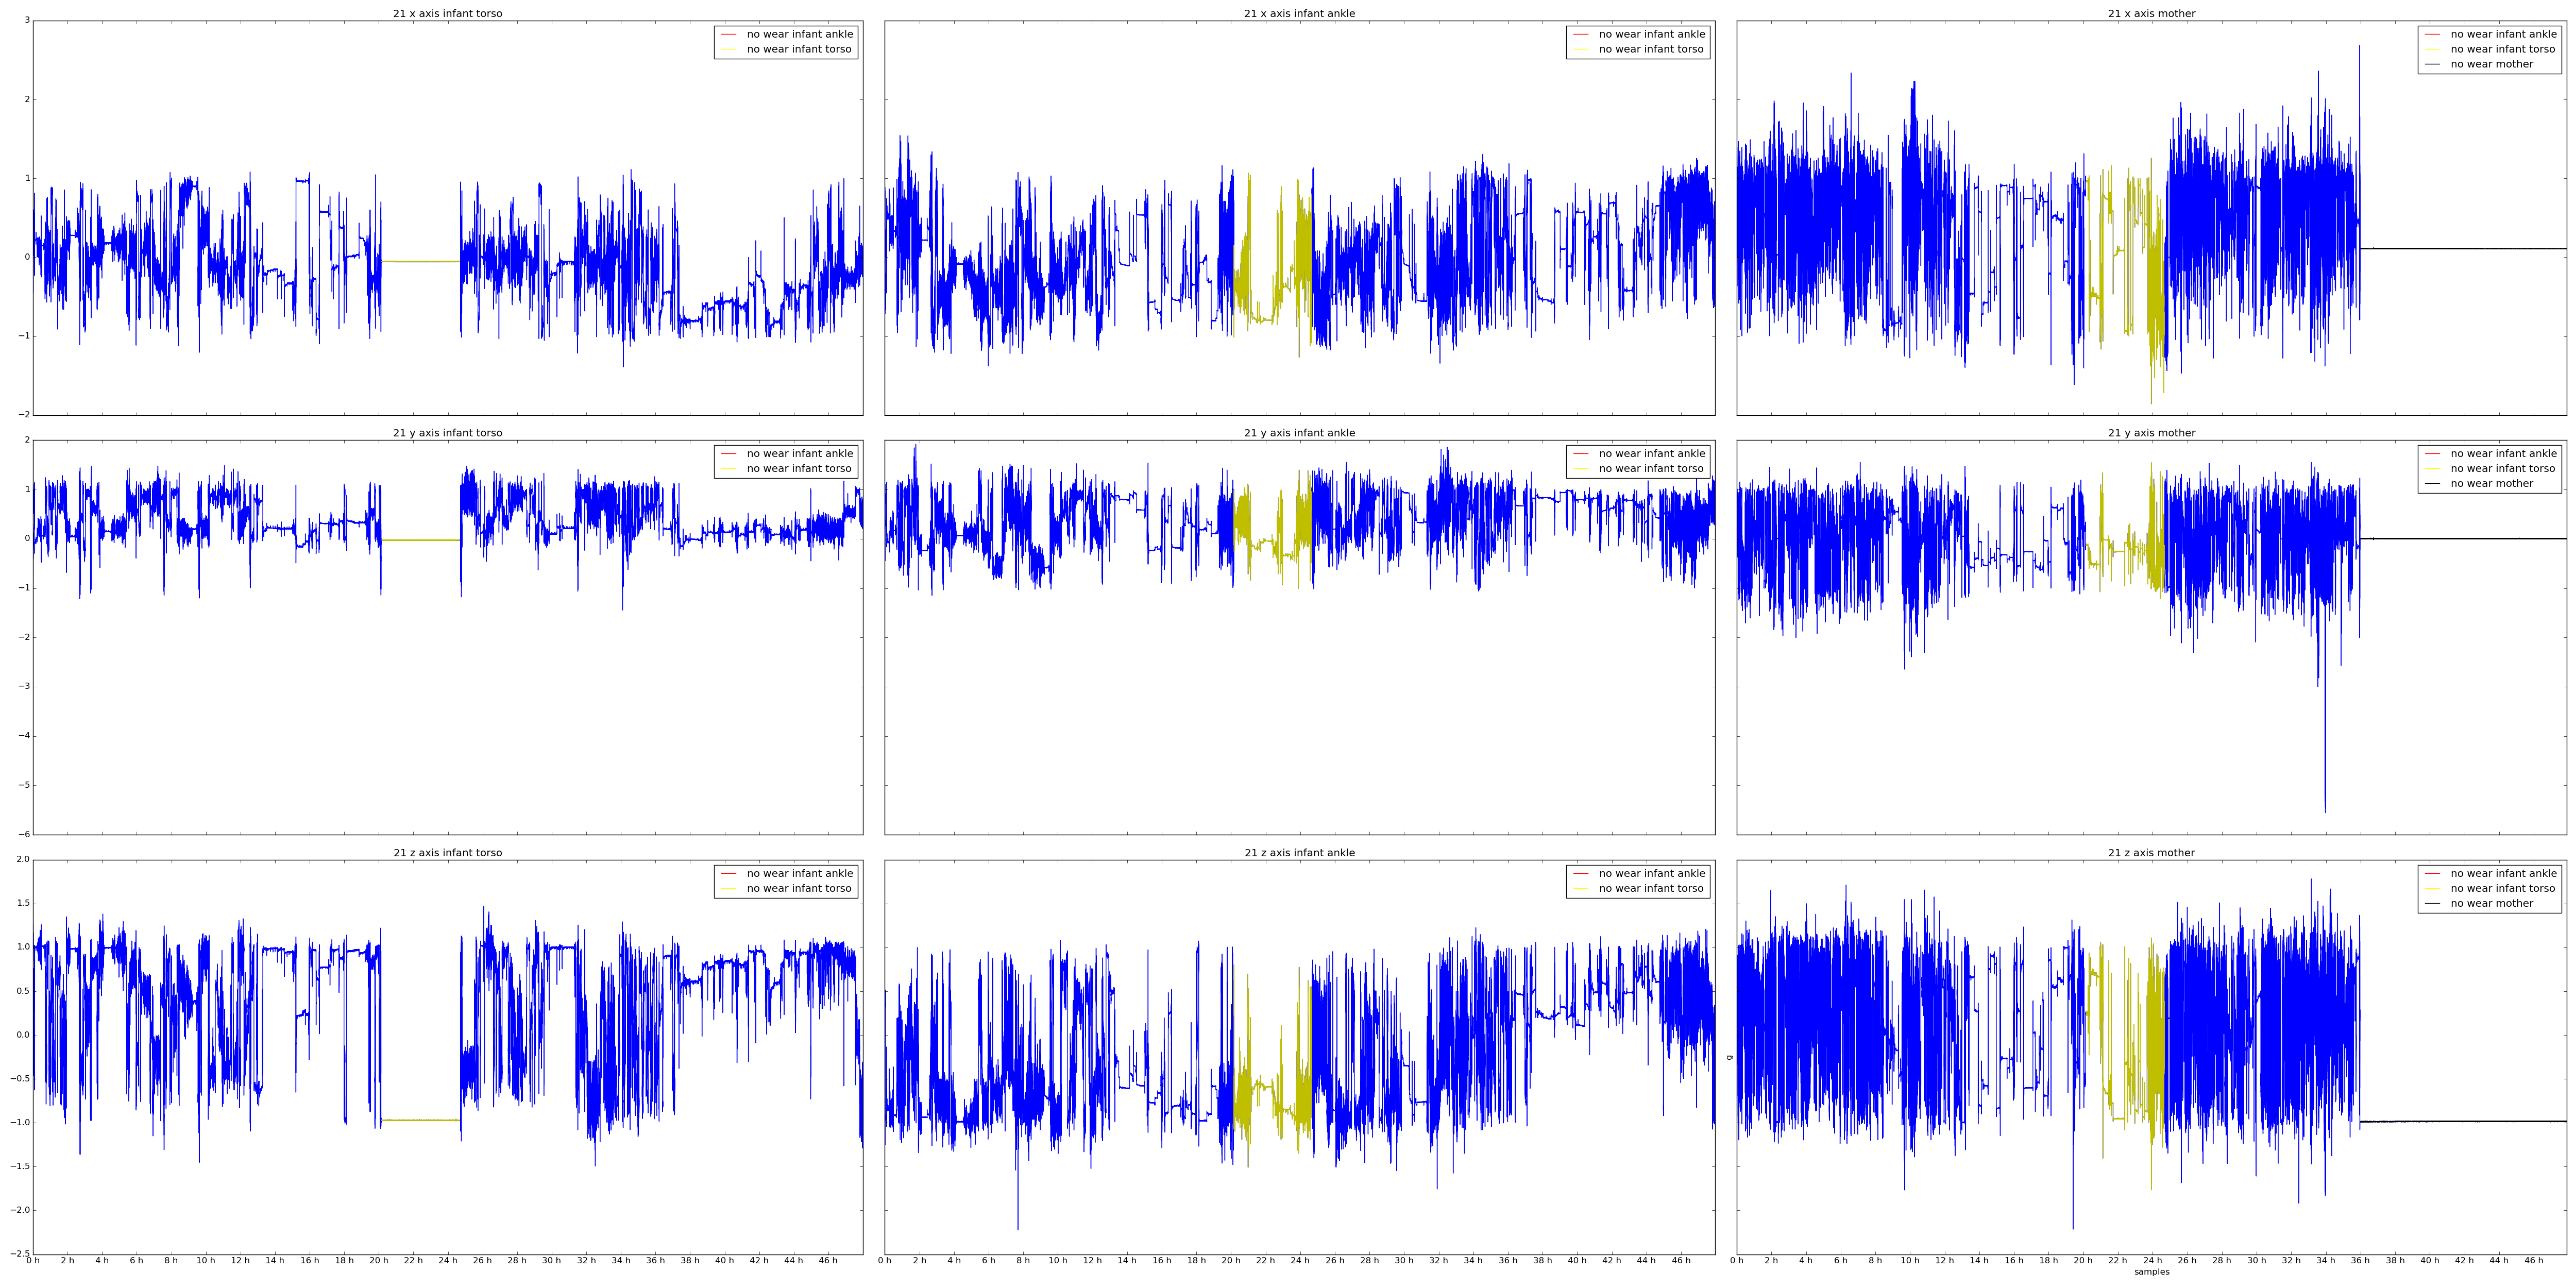
\includegraphics[width=15cm, height=8cm]{21NoWearTimeLabeled.png}
\caption{Example of accelerometer data for one infant-mother pair. The x, y and z axis are aligned vertically, while the infant torso, infant ankle and mother wrist measurements are aligned horizontally. The yellow color represents infant torso non-wear time, which is subsequently colored in the rest of the measurements and the black color represents maternal non-wear time, which is colored only in maternal measurement.}
\end{figure}
\\
Based on trial and examination of the results and the previously set cut points \cite{ref2}, the window length is set to 30 minutes, which corresponds to 72000 data points. Shorter windows are more prone to classify time windows of sleeping as non-wear time, whereas larger windows failed to detect short duration of non-wear time. SD threshold is set to 0.002 g and minimum to maximum span threshold is set to 0.015 g. To increase accuracy even further, a more detailed windowed examination is performed around the edges to better detect the borders of the blocks of non-wear time, and up to three windows of in between blocks of non-wear time are set as non-wear. 
Upon final inspection of the results and their plots, all visually apparent non-wear blocks are detected, with a few minor blocks that are likely to be sleeping blocks based on the time of occurrence. 
\newpage
\subsection{Summary derivation}
Accelerometers can be designed to measure acceleration on a single axis, dual axes or three axes along with different sampling rates. For the accelerometer used in this project (GENEA), it has been shown that sampling frequencies larger than 10 Hz and/or more than one axis do not significantly increase classification accuracy, when classifying 10-12 semistructured activities performed in the laboratory or an outdoor environment, while wearing the accelerometer on the right wrist\cite{ref7}. Considering infants movement is not structured and accelerations were recorded in a free living environment with an unpredictable pattern, the use of three axes is justified by the need to record the accelerations in the three dimensional space, to ensure the analysis design and implementation is not restricted or disabled by the lack of available information. On the other hand, having three axis and a high sampling rate, the amount of noise present in the final outcome can be higher, if the data is not filtered and summarized properly. Another issue arises when comparing the outcome of two accelerometers. The way the ankle and torso accelerometers were placed, the three axes of the two accelerometers were not aligned and with the mobility of the infants ankle they were liable to rotations. This presents a problem, since each of the axes should be aligned prior to the analysis.\\
For the reasons given above, a summary over all three axis has to be derived. Summary derivation can have a significant impact on the final results. Although it has been shown that different summaries can have a similar PA prediction accuracy, the amount of variance interfered by summarization can differ significantly \cite{ref3}.
Two types of summary derivations are performed and examined in this project. First is the averaged Euclidean norm of the median filtered three axis, followed by a subtraction of one, to correct for the gravitation. Second is an averaged Euclidean norm of the Butterworth bandpass filtered and median filtered three axes.\\
Averaging is done over one second, with the purpose of removing the noise. The width of the median filter is 11 and its purpose is to remove any spikes from the measurement which are due to noise. Bandpass filter is set to allow frequencies from 0.5 to 15 Hz, since changes occurring at a faster paste then 15 times a second are most probably due to noise, while changes occurring slower then once per two seconds are actually baseline shifts due to gravitational measure shifting between the axes in rotations.\\ When plotting the derived summary for torso and ankle, one can clearly see the substantial similarities in the measurements due to the caretakers contributions, example for the first summary derivation in Figure 2. 
\\
While the infant torso and ankle derived summaries show substantial similarity, the corresponding derived summary, of the maternal accelerometer data, only exhibits the same pattern of activity as the infant during the night, indicating plausible interaction between the mother and her infant, example in Figure 3.
\newpage
\begin{figure}[h!]
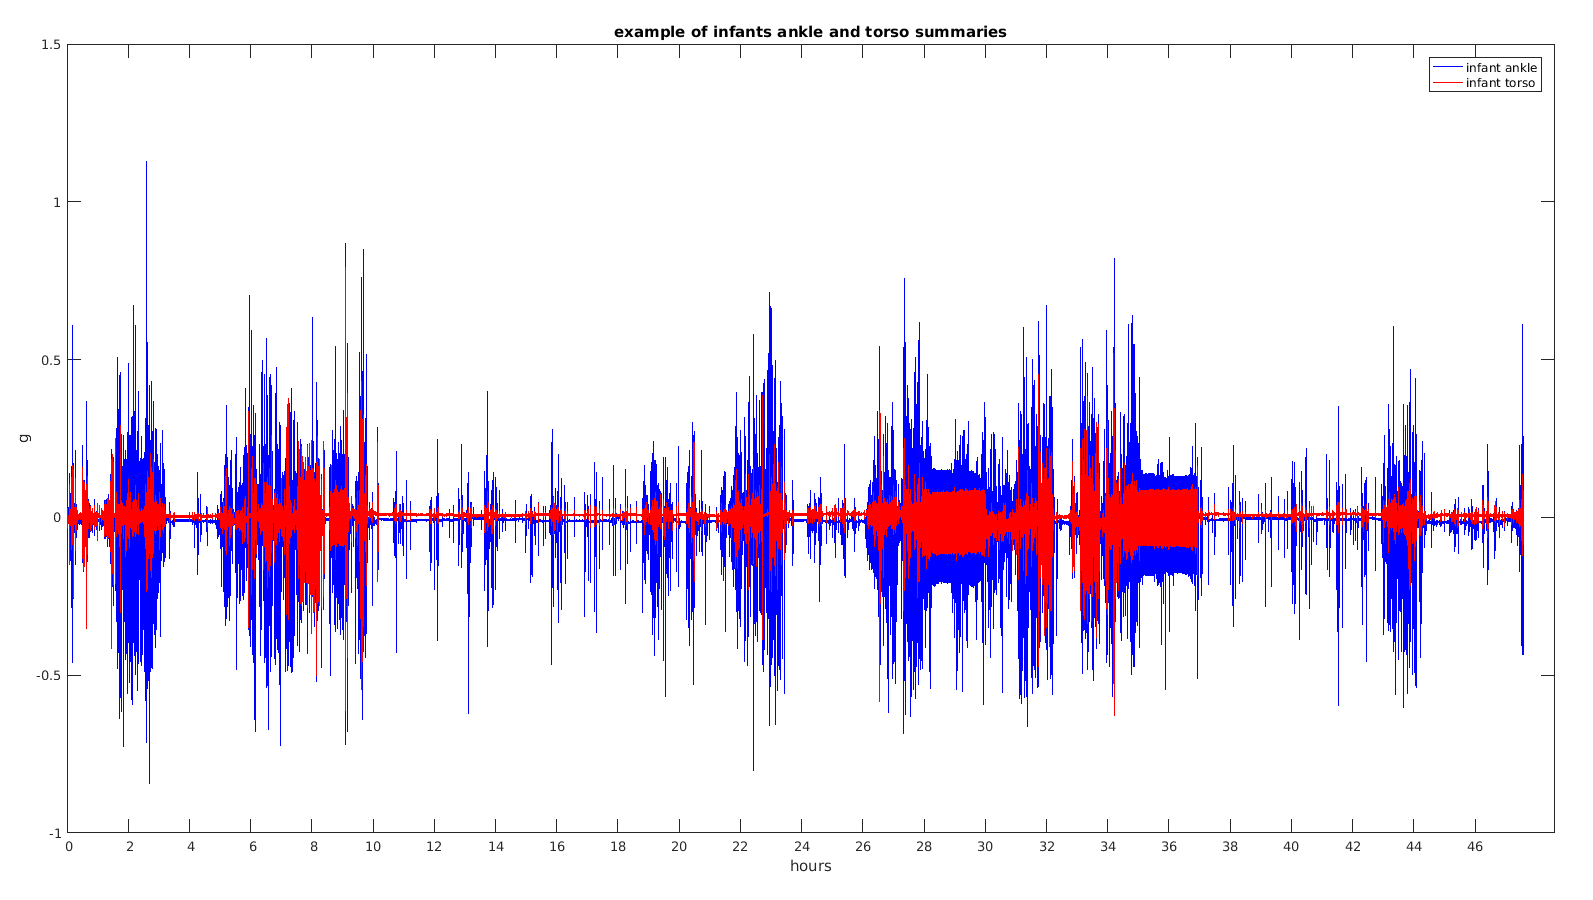
\includegraphics[width=15cm, height=7cm]{exampleTorsoAnkle.png}
\caption{An example of the first summary derivation over all three axes for infant torso and infant ankle measurement, illustrating the degree of similarity in activity patterns, with visible leftovers of the gravitational acceleration.}
\end{figure}

\begin{figure}[h!]
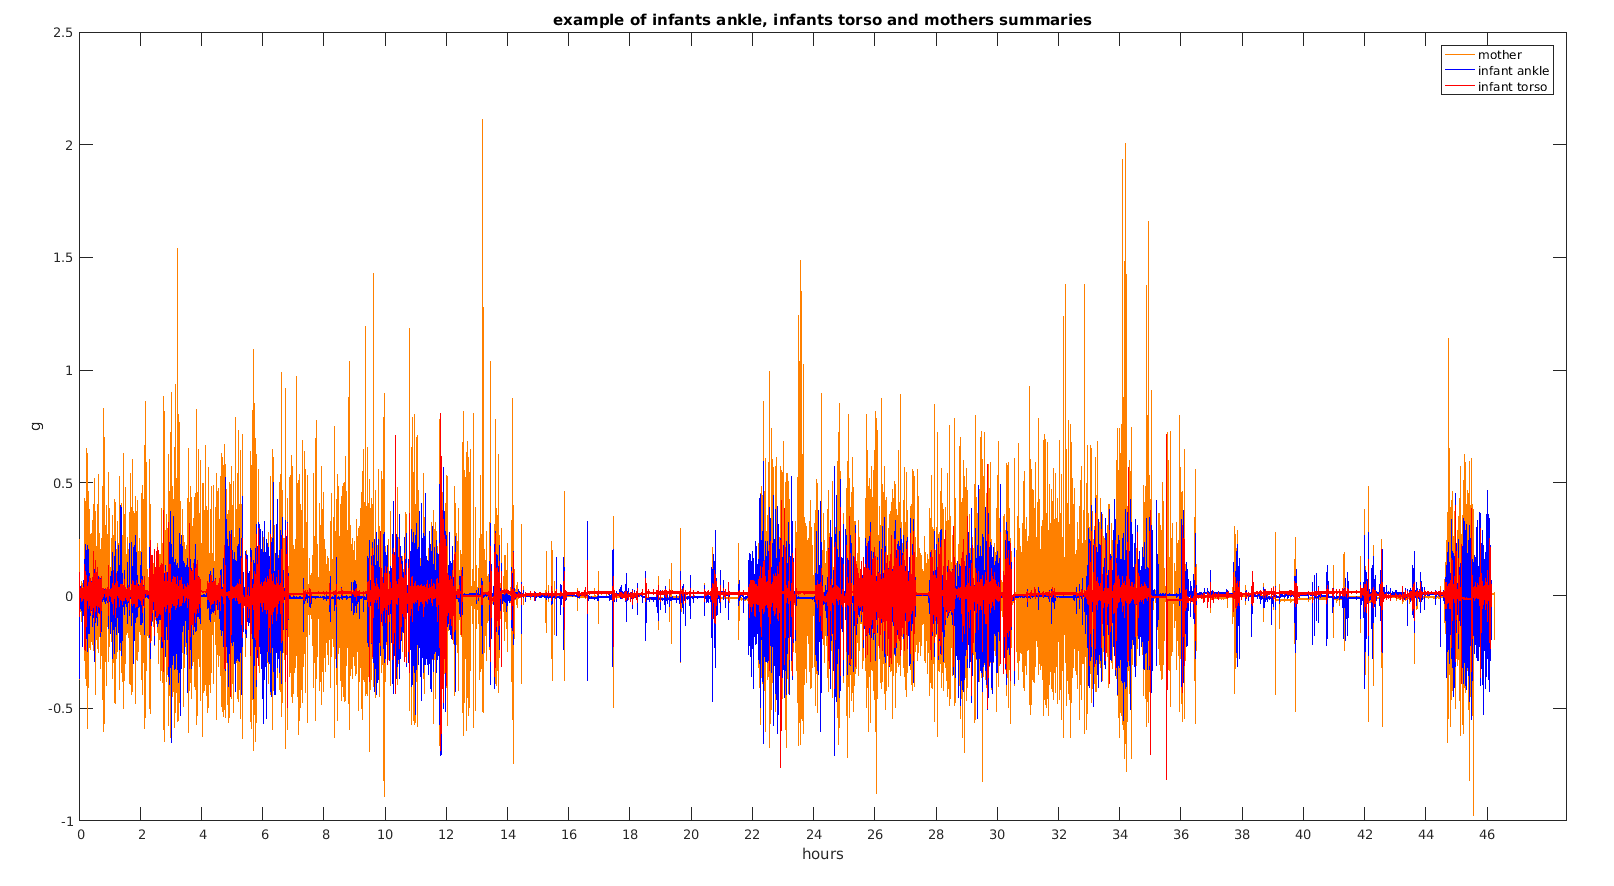
\includegraphics[width=15cm, height=7cm]{exampleTorsoAnkle2.png}
\caption{An example of the first derived summaries of infant ankle, infant torso and maternal wrist measurements, illustrating the degree of similarity in activity patterns across night and day, with visible leftovers of the gravitational acceleration.}
\end{figure}
\\
In Figure 2 and 3 one can observe the remaining baseline shifts, due to leftovers of the gravitational accelerations in the first derived summary, that need further removal, which is discussed in the next subsection. \\
Although the principals in both summary derivations are commonly used in accelerometer data processing, they are fundamentally very different and so is their outcome. The lack of established consensus regarding an optimal summary derivation is an ongoing issue in accelerometer data processing and analysis. Same example as in Figure 2 is shown for the second summary derivation in Figure 4, showing substantial differences, which are expected, based on the fundamental differences of the principals used.
\begin{figure}[h!]
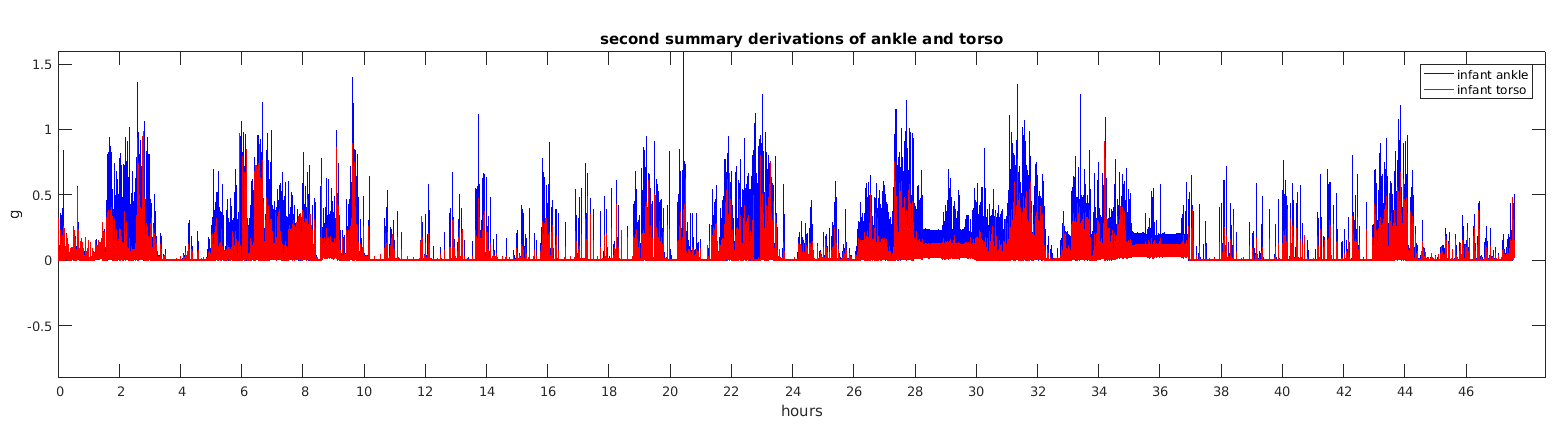
\includegraphics[width=15cm, height=6cm]{bandpass_summary_example.png}
\caption{An example of the second summary derivation over all three axes for infant torso and infant ankle measurement.}
\end{figure}
\\
The two different types of summary derivation are therefor included in the analyses in order to asses the amount of variance interfered and choose the best to use for PA extraction.
\\
\subsection{Gravity component}
The separation and removal of the gravitational component becomes more complicated when rotations are present in the measurement \cite{ref3}. This can result in less accurate further processing, especially when outcomes from different accelerometers have to be compared. In the first summary derivation, the impact of the gravitational acceleration is intended to be removed by subtracting one from the final norm, while in the second summary derivation, the impact of the gravitational acceleration is intended to be removed by the high pass component of the bandpass filter. By examining the outcomes of the first summary derivation, left-overs of the gravitational impact are clearly visible, while in the second summary derivation, left-overs from the gravitational impact are not clearly visible which makes it more difficult to asses their quantity and form, making further correction challenging. Taking only the first summary derivation into consideration, further corrections can be made to ensure that the measurement does not reflect the influence of gravitation. By simply correcting the baseline to zero, the left-over impact of the gravitational acceleration can be reduced in the first derived summary, example in Figure 5. 
\newpage
\begin{figure}[h!]
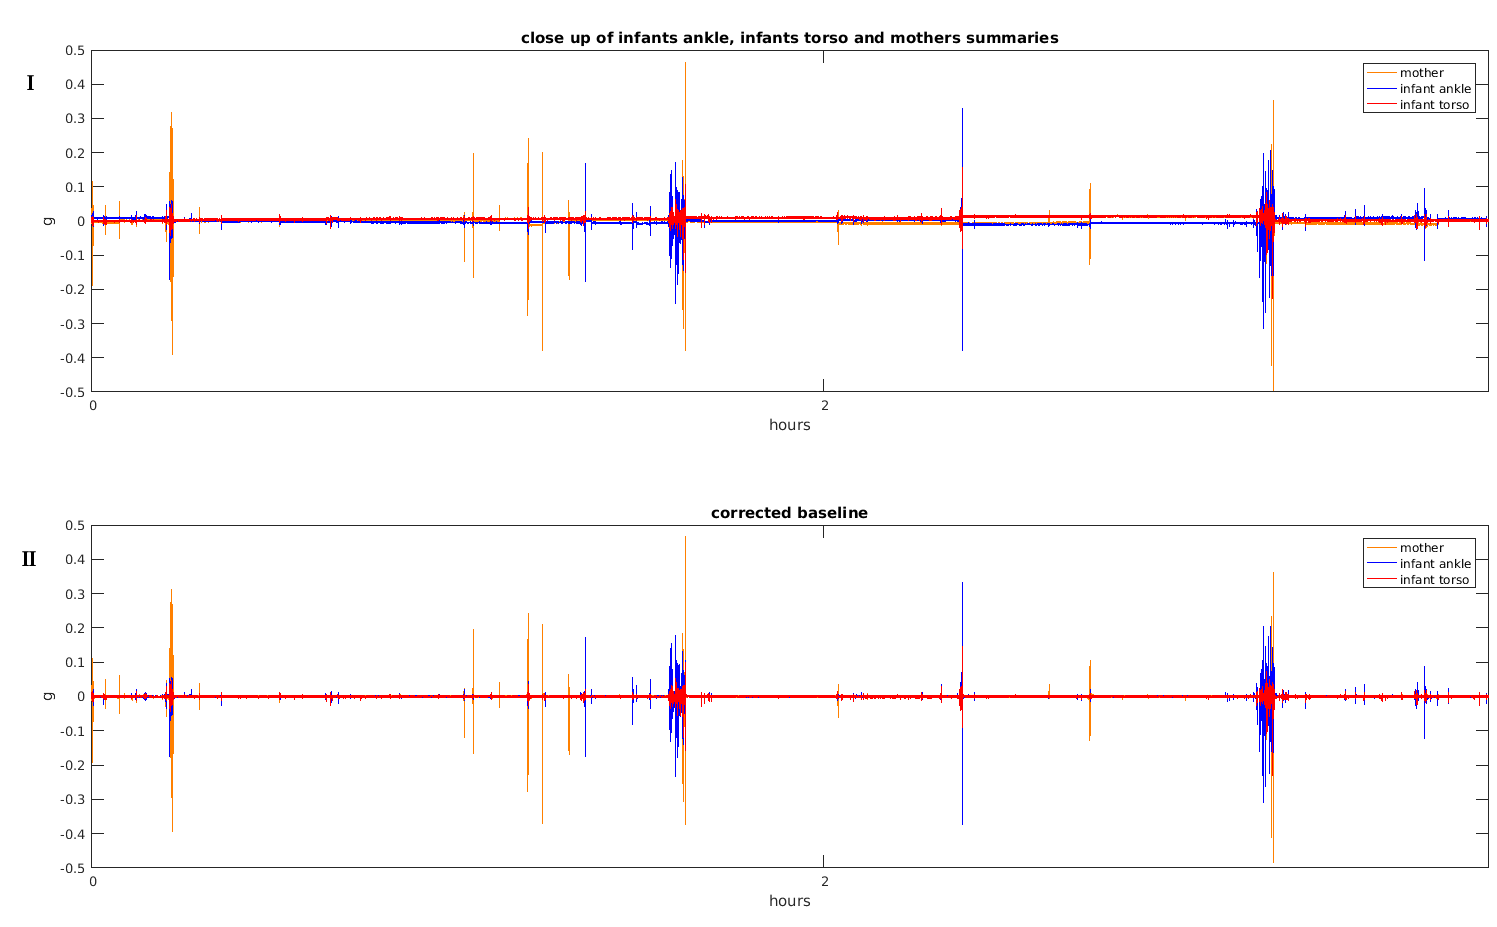
\includegraphics[width=15cm, height=10cm]{exampleTorsoAnkle5.png}
\caption{An example of a close up of the first summary derivation for infant torso, infant ankle and maternal wrist accelerometer data, before (I) and after (II) the baseline correction.}
\end{figure}
\\
\\
Baseline correction is implemented in Matlab based on a smoothing method with penalized least squares\cite{ref4}. The method is an extension of the Whittakers method for smoothing, which works by minimizing the following sum: 
\begin{equation}
S=\sum_{i} (y_i - z_i)^2 + \lambda\sum_{i} (z_i - 2z_{i-1} + z_{i-2})^2\thinspace \thinspace ,
\end{equation}
where \textit{y} is the input signal, \textit{z} is the final smoothed signal and \textit{i} goes through the data points.
The first part of the sum ensures the best approximation of the input signal, while the second part represents the penalty for non-smoothness. 
In practice $\lambda$ is set from $ 10^{2} \leq \lambda \leq 10^{9}$ and its value depends on the input data and the desired final result. Since the goal of the baseline correction in the project is to keep all the amplitudes intact, but only correct the global baseline, $\lambda$ is set to $10^{9}$.
\\
Reformatting the above into a linear system of equations, we get:
\begin{equation}
(I + \lambda D'D)z = y\thinspace \thinspace ,
\end{equation}
where I is the identity matrix and D is its differential matrix. 
The computational time and space can be optimized, using sparse matrices and Cholesky factorization. The resulted over-smoothed signal represents the baseline and is therefor subtracted from the measurement. This way, the amplitudes remain intact, but the baseline drifts and jumps are removed and the signal baseline is set to zero. 
\subsection{Caretakers contributing accelerations}
The accelerometer is liable to pick up any acceleration caused by the subject moving, regardless if the subject is in PA or is being moved by another person. Infants at four months of age are completely dependent on the caretaker. Besides the basic tasks like feeding, bathing, dressing, etc., the infants at four months of age require a substantial amount of carrying, placing and cradling. This results in significant contributions of accelerations caused by the person caring for the infant\cite{ref1}\cite{ref5}\cite{ref6}.\\In one of the previous studies of infants PA\cite{ref5}, the results also showed that contributed accelerations differed significantly between the three differently placed accelerometers, when in fact recording the \textit{same} activity, while the contributed accelerations could add up to more than a half of the detected activity. \\Caretakers contributing accelerations were considered in the study design of this project. Two accelerometers were placed on the infant, one on the torso and one on the ankle, to detect when the infant is being active or is being moved. The rationale behind the idea was that infants at four months of age can not move the torso, so large accelerations recorded on the torso placed accelerometer should be due to caretakers contributions. Two strategies, removing caretakers contributions, were planned when designing the study. First, considering the larger accelerations on the torso placed accelerometer are mainly due to caretakers contributions, one could simply subtract the torso placed measurement from the ankle placed measurement, resulting in the remaining accelerations on the ankle placed accelerometer being due to infants PA only. Second, since the periods of increased accelerations on the torso placed measurement are mainly due to caretakers contributions, one could simply remove these periods from the ankle placed measurement, to ensure that the remaining accelerations on the ankle placed accelerometer are due to infants PA only.\\In years following the study design, a related scientific article\cite{ref1} and a conference abstract\cite{ref5} were published, the latter being followed by a PhD-defense\cite{ref6}. The results of these researches are very informative for the current project, since they raise doubt about the planned two strategies, exposing several faults. Based on the exploration of infants accelerometer data at hand and results from related researches, published after the current study was designed, it was clear that caretakers contributions are recorded differently between the differently placed accelerometers. This is in contrast with the first strategy of simple subtraction. Not only that the caretakers contributions would not be removed, additional noise might be added, while larger accelerations due to caretakers contributions could occur on the torso placed measurement, resulting in a negative outcome of subtraction. The second strategy of complete removal of caretakers contributing periods is therefore more promising. Nevertheless, keeping in mind that infants at four months will spend most of their time being moved, this strategy is in risk of loosing most of the measurement, while the resulting outcome might be limited to the time the infant was sleeping. With these observations in mind, several more advanced and complicated approaches are designed and tested along with the originally planned. In total, the following approaches are tested:
\begin{itemize}
\item \textbf{A.} Simple subtraction of ankle and torso placed measurements
\item \textbf{B.} Subtraction of windowed intensities of ankle and torso placed measurements
\item \textbf{C.} Correction based on windowed intensities of ankle and torso placed measurements
\item \textbf{D.} Correction based on correlated windowed intensities of ankle and torso placed measurements
\item \textbf{E.} Complete removal of periods, where caretakers contributing accelerations are assumed
\end{itemize}
\\In approach \textbf{A} the derived summary from the torso placed measurement is simply subtracted from derived summary of the ankle placed measurement. Example of a result from approach \textbf{A}, using the first summary derivation is shown in Figure 6, where it is apparent, that simple subtraction is not efficient, but rather amplifies the contributing accelerations.
Example of the same result, but using the second summary derivation is shown in  Figure 7, showing substantially different, but nevertheless still inefficient and inappropriate results, where analysis is required to asses whether the results from the two types of summary derivations are even comparable.
\begin{figure}[h!]
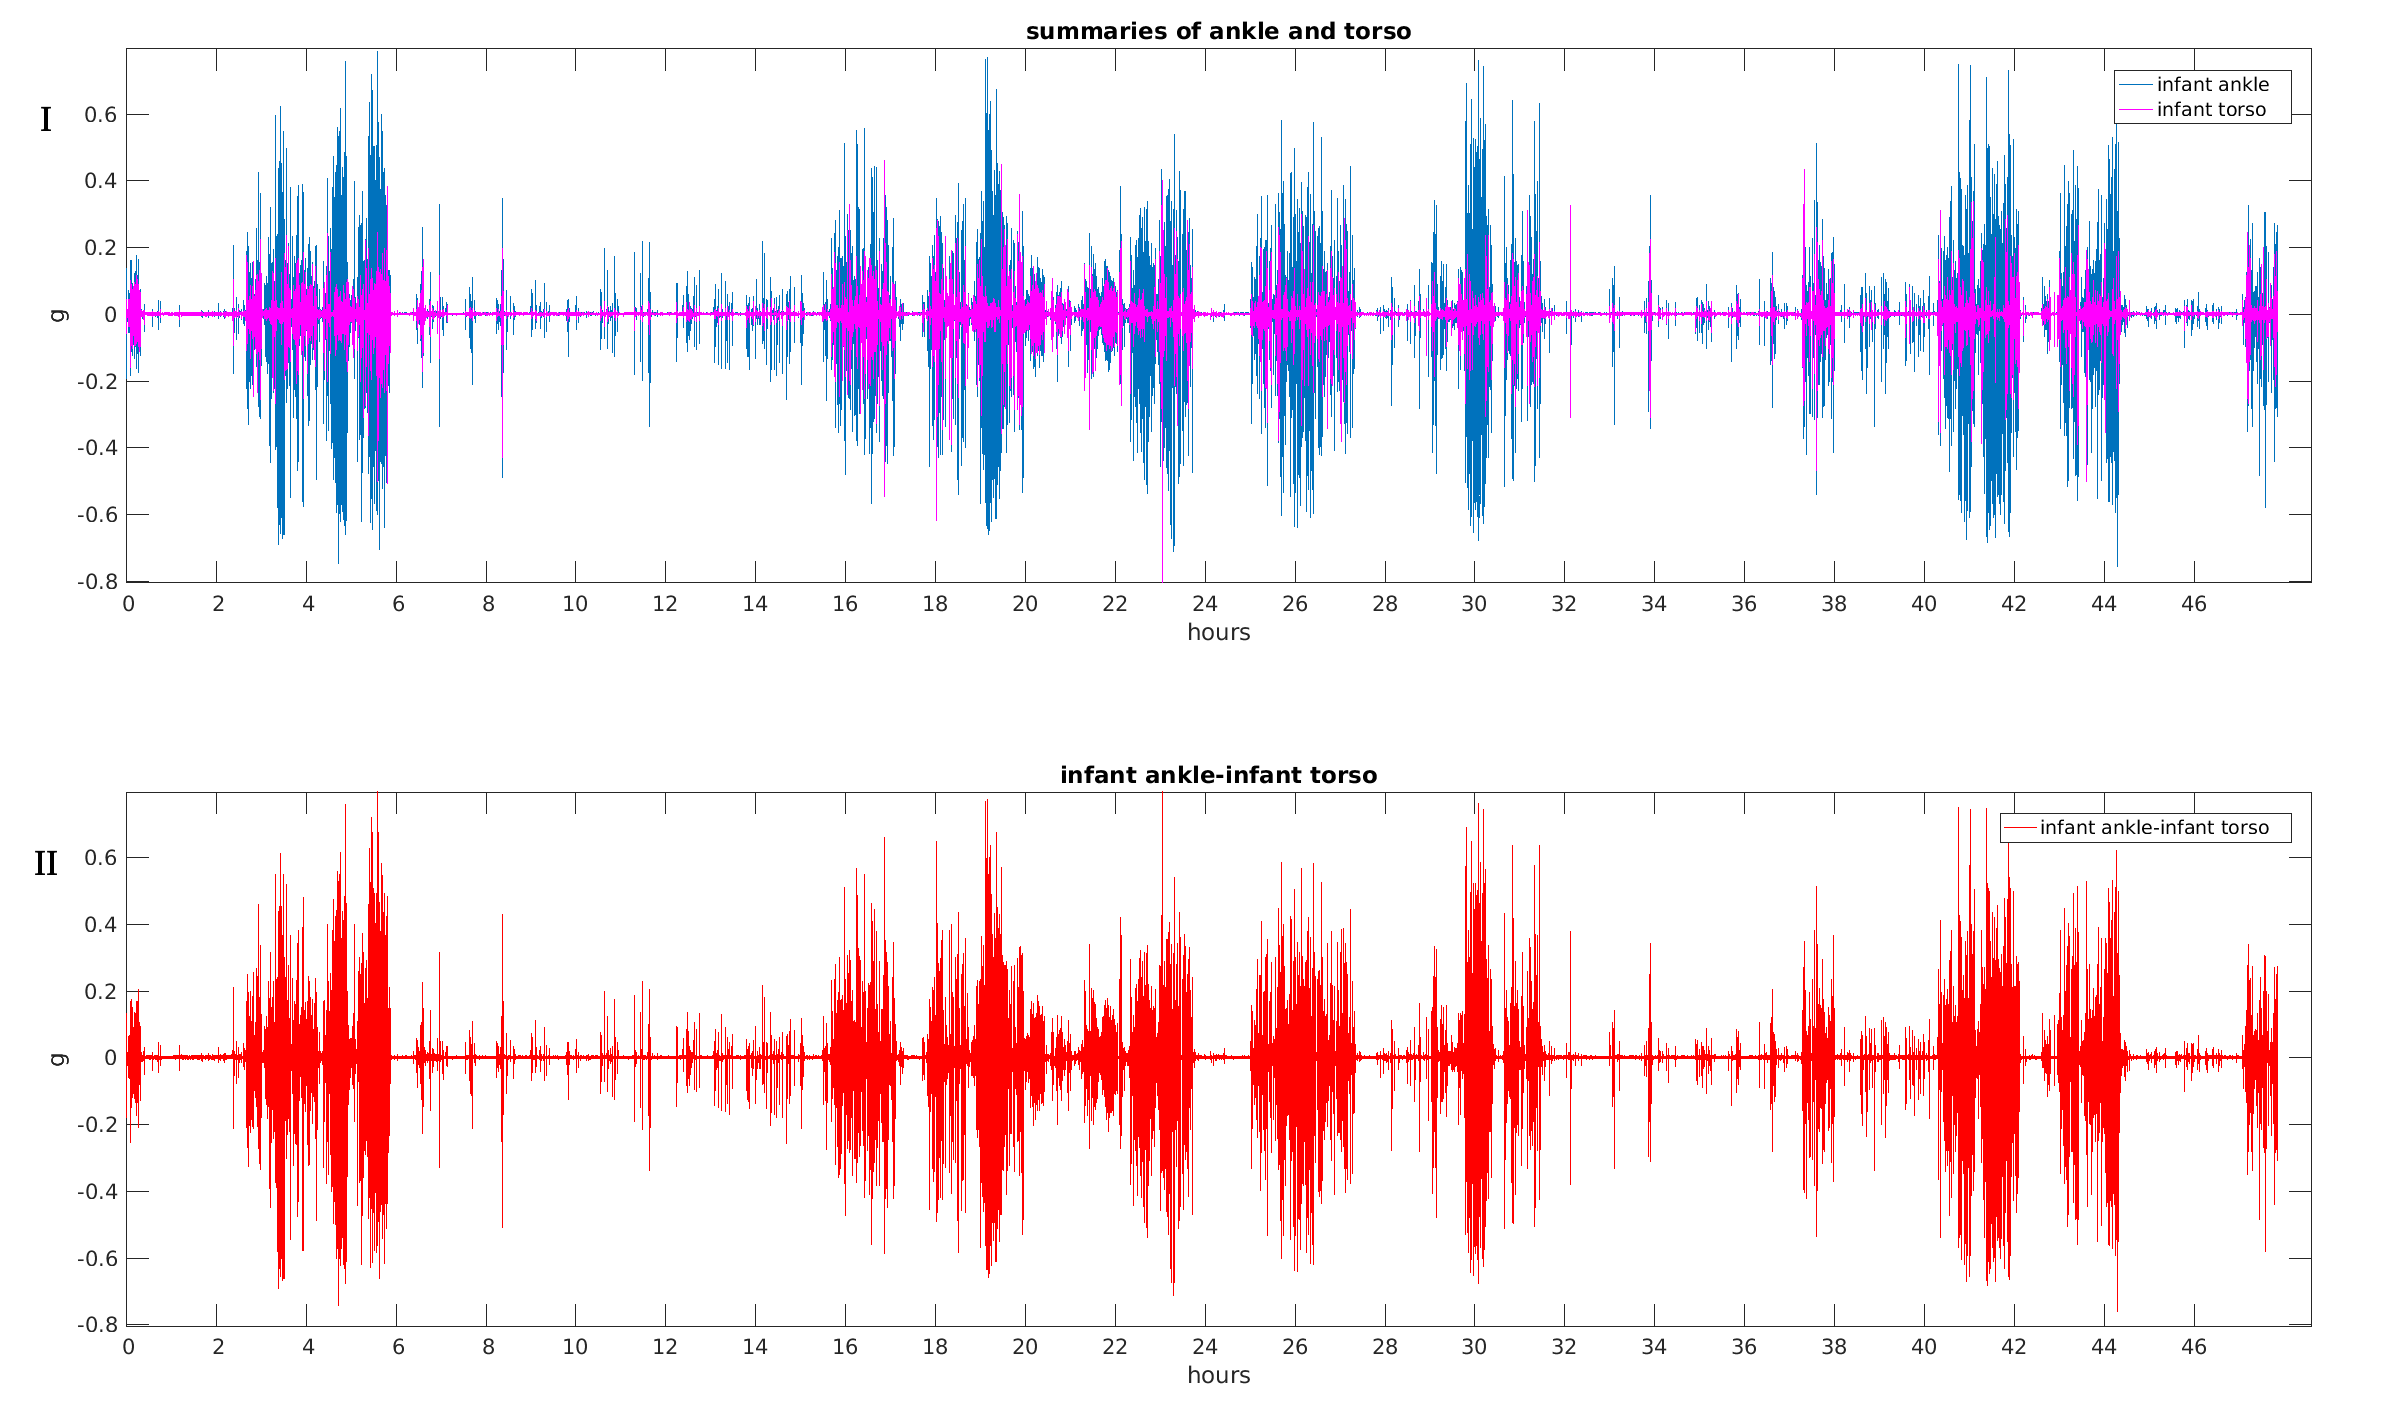
\includegraphics[width=15cm, height=8cm]{SimpleSubtracting.png}
\caption{A plot exhibiting the first summary derivations of the torso and ankle placed measurements (I) and the result of a simple subtraction of the torso placed measurement from the ankle placed measurement (II).}
\end{figure}
\begin{figure}[h!]
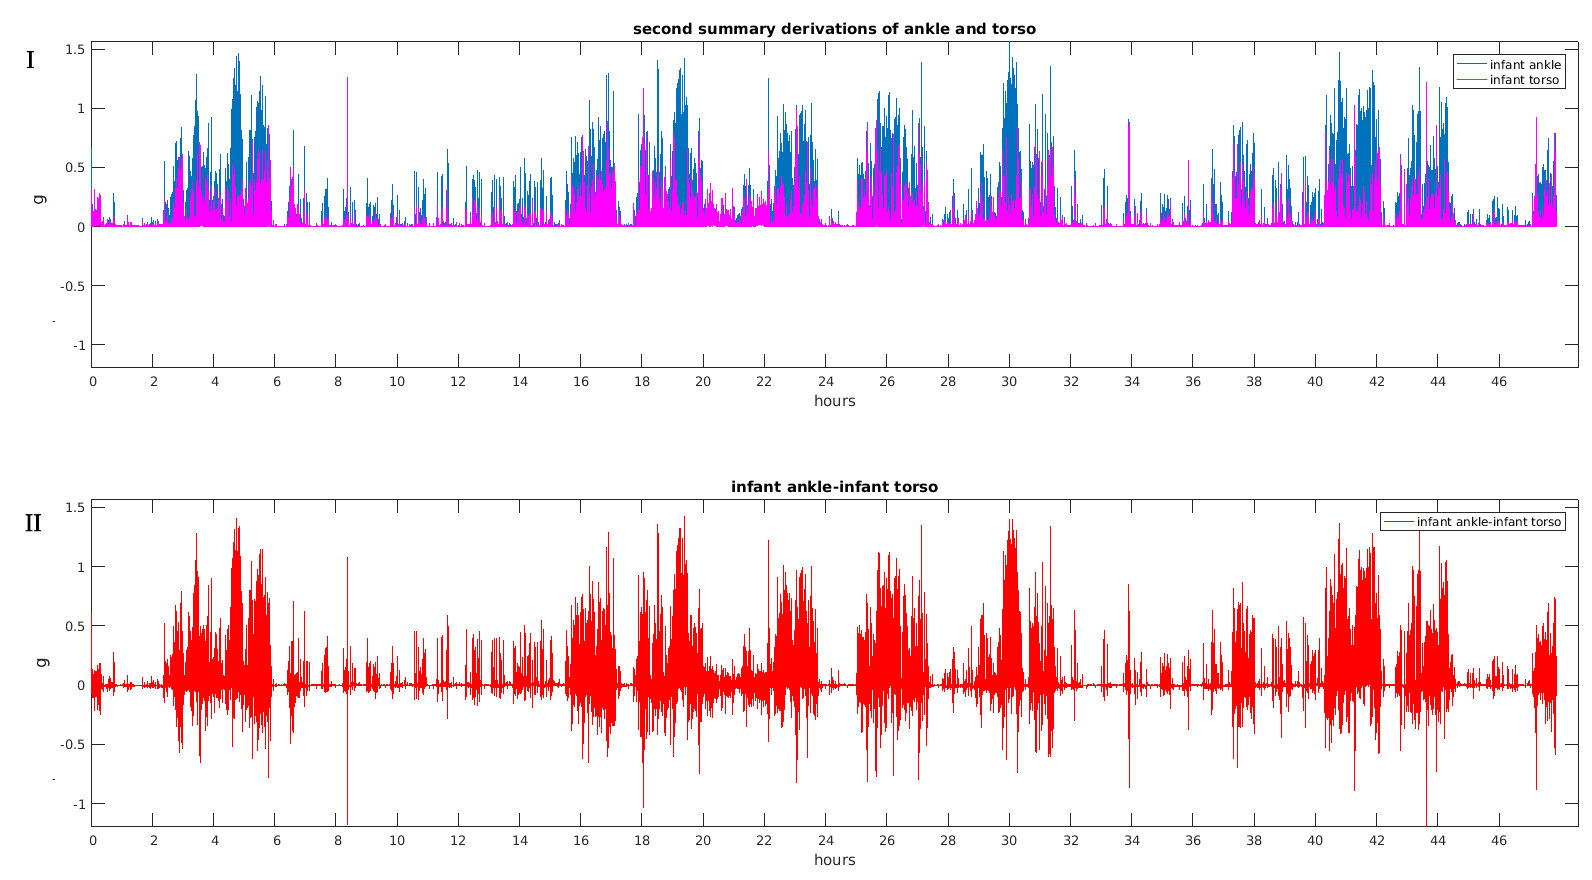
\includegraphics[width=15cm, height=8cm]{bandpassJustSummary_and_A.png}
\caption{A plot exhibiting the second summary derivations of the torso and ankle placed measurements (I) and the result of a simple subtraction of the torso placed measurement from the ankle placed measurement (II).}
\end{figure}
\newpage
As the measurements exhibit a substantial amount of similarity on a large scale, but seem to be too different point to point, the second (\textbf{B}) and third (\textbf{C}) approaches use an even more summarized measure, derived by calculating windowed absolute intensities. Specifying window length as \textit{k} and measurement length as \textit{n}, we get  \( \frac{n}{k} \)  windows, for which the absolute intensity (AI) is calculated as following:
\begin{displaymath}AI=\frac{1}{k}\sum_{i=1}^{k}|s_i|\end{displaymath} where \textit{s} is taken from the derived summary of the acceleration measurement.\\
In approach \textbf{B} the absolute intensities of the torso placed measurement are again simply subtracted from the absolute intensities of the ankle placed measurement. In approach \textbf{C}, the loss of resolution by further summarization is improved. The improvement is done by using the point to point ratio, between the windowed absolute intensities of the torso and ankle placed measurement, as a factor by which all the points in the corresponding window of the original summary derivation of the ankle placed measurement are decreased. For example, if the torso absolute intensity is half the ankle intensity, all the points in the corresponding window of the original summary derivation of the ankle placed measurement are decreased by a half of their size. The process is implemented in Matlab, where the window length is set to 2400 data points, which corresponds to one minute of measurement. Examples of a result in approach \textbf{B} and \textbf{C}, using the first original summary derivation are shown in Figure 8 and Figure 9, respectively. Examples of a result in approach \textbf{B} and \textbf{C}, using the second original summary derivation are shown in Figure 10 and Figure 11, respectively. Comparing with the approach \textbf{A}, the results from the two types of summary derivation appear less different in approaches \textbf{B} and \textbf{C}, which is examined with further analysis. 
\begin{figure}[h!]
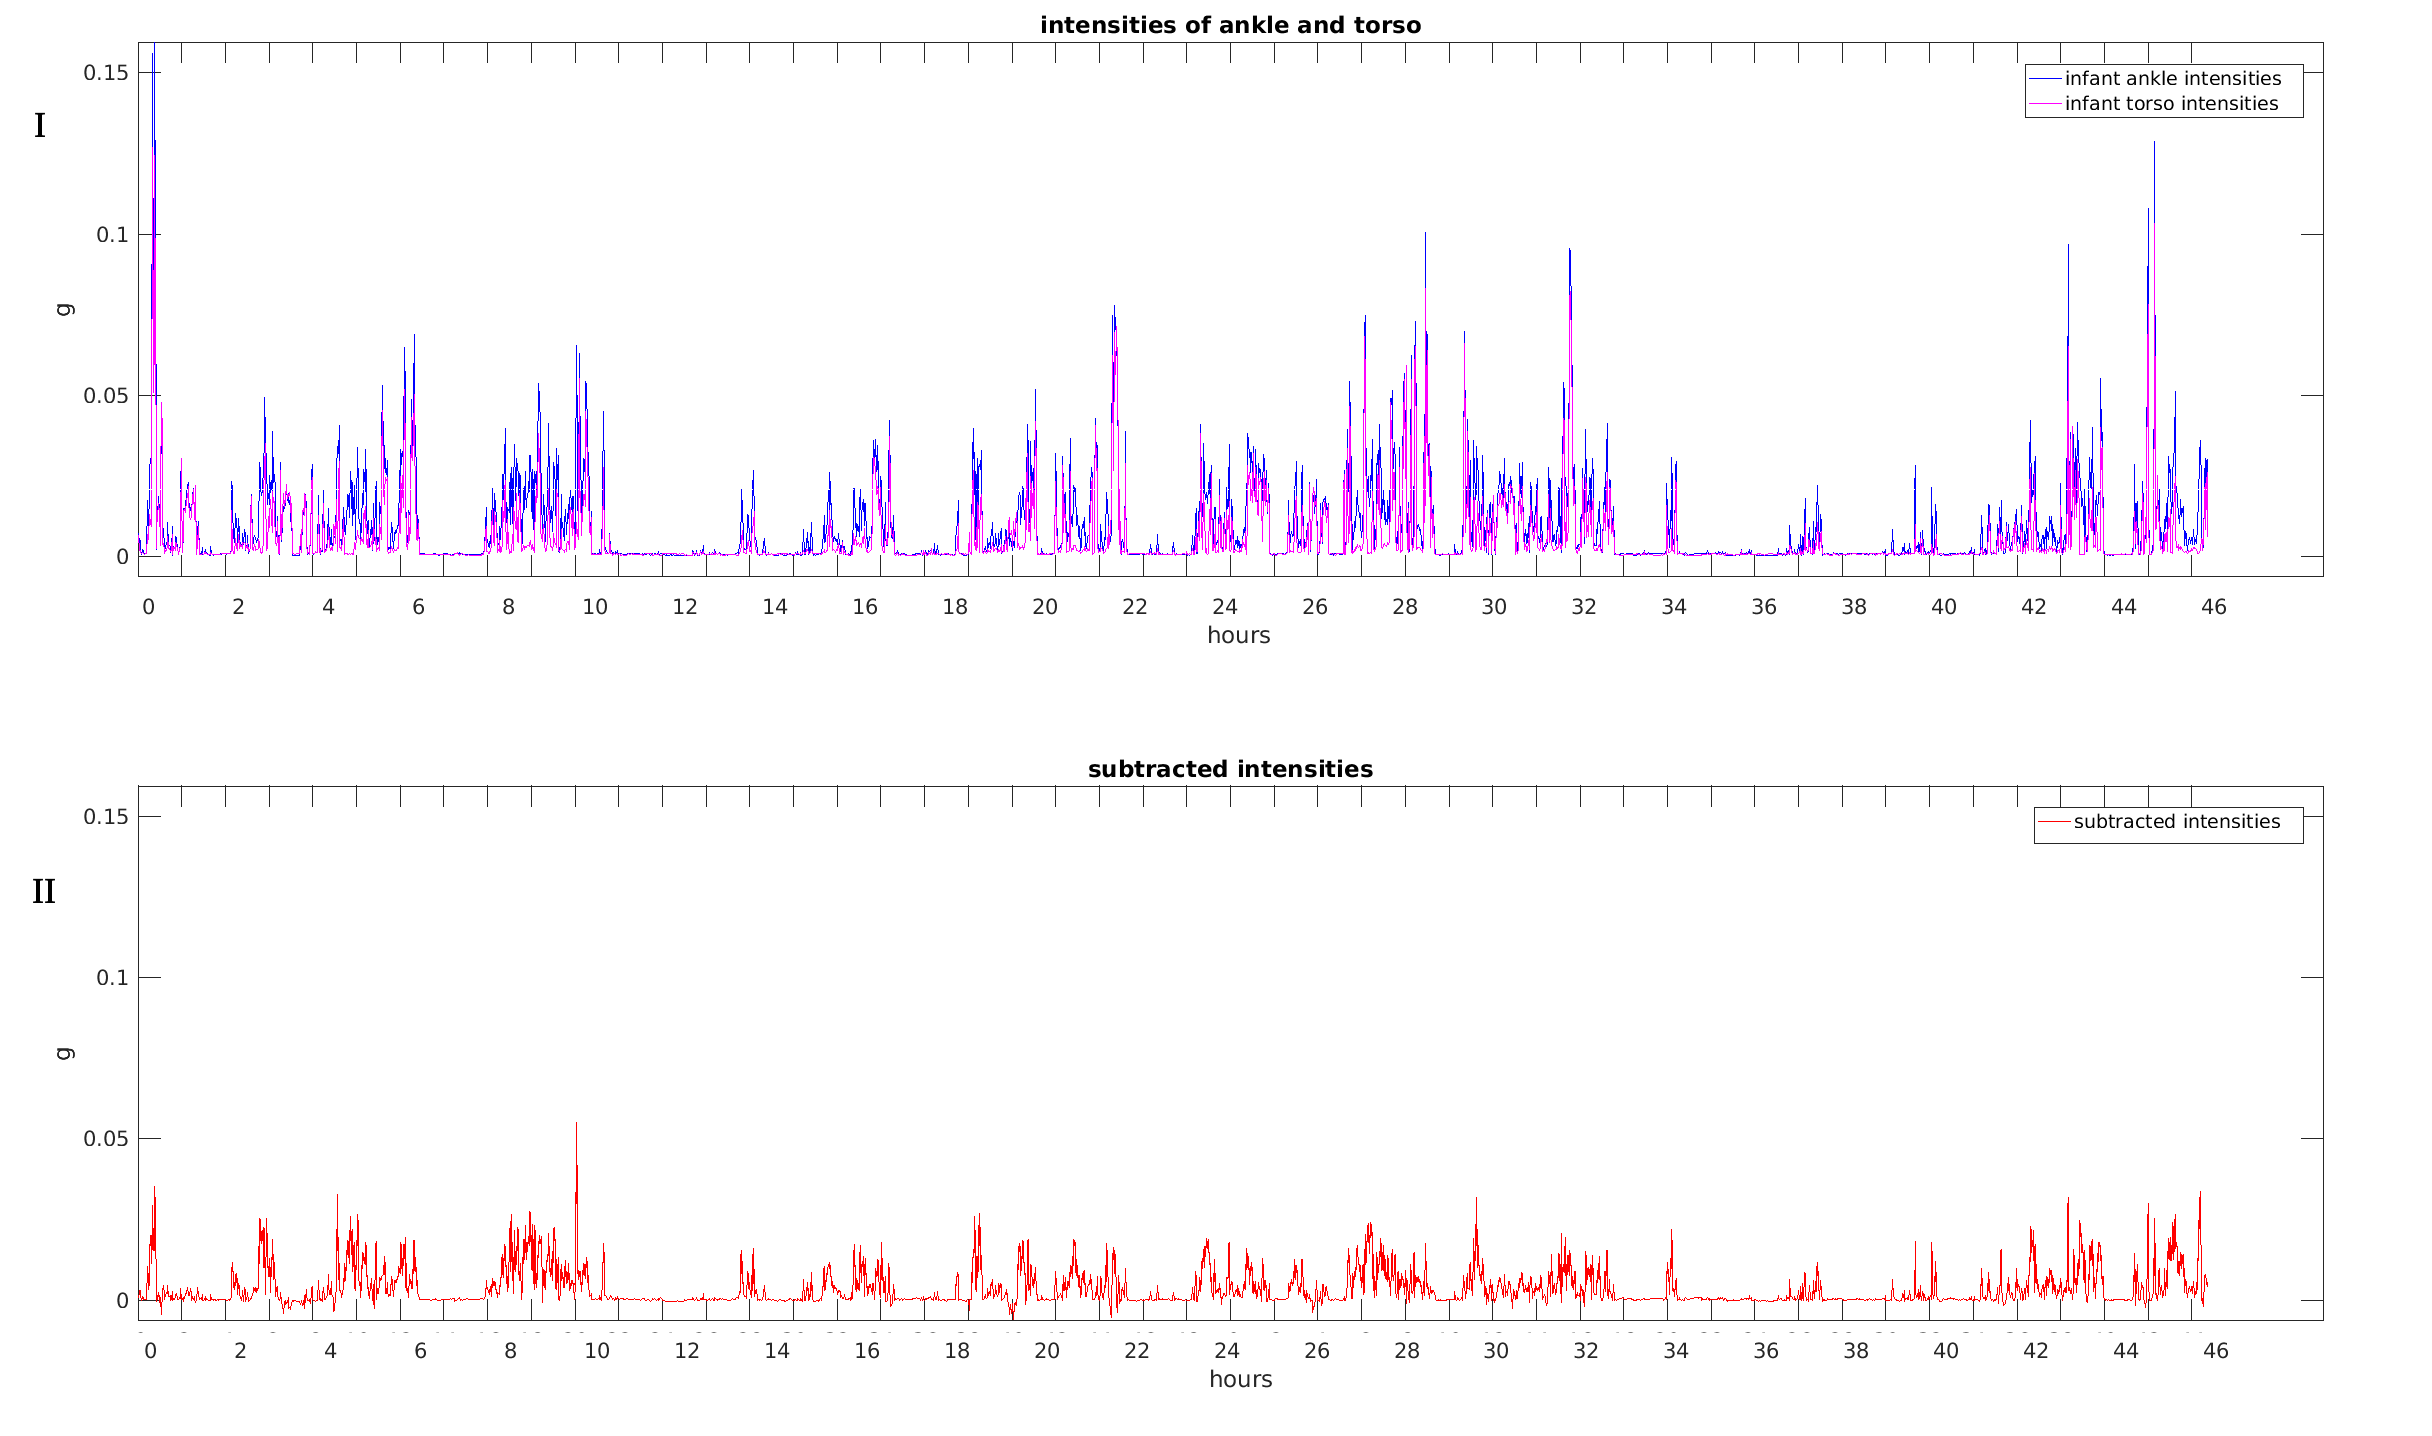
\includegraphics[width=15cm, height=7.5cm]{subtractedIntensities.png}
\caption{An example of windowed absolute intensities obtained from the first summary derivations of torso and ankle placed measurements (I) and the result obtained by subtracting the windowed absolute intensities (II).}
\end{figure}
\begin{figure}[h!]
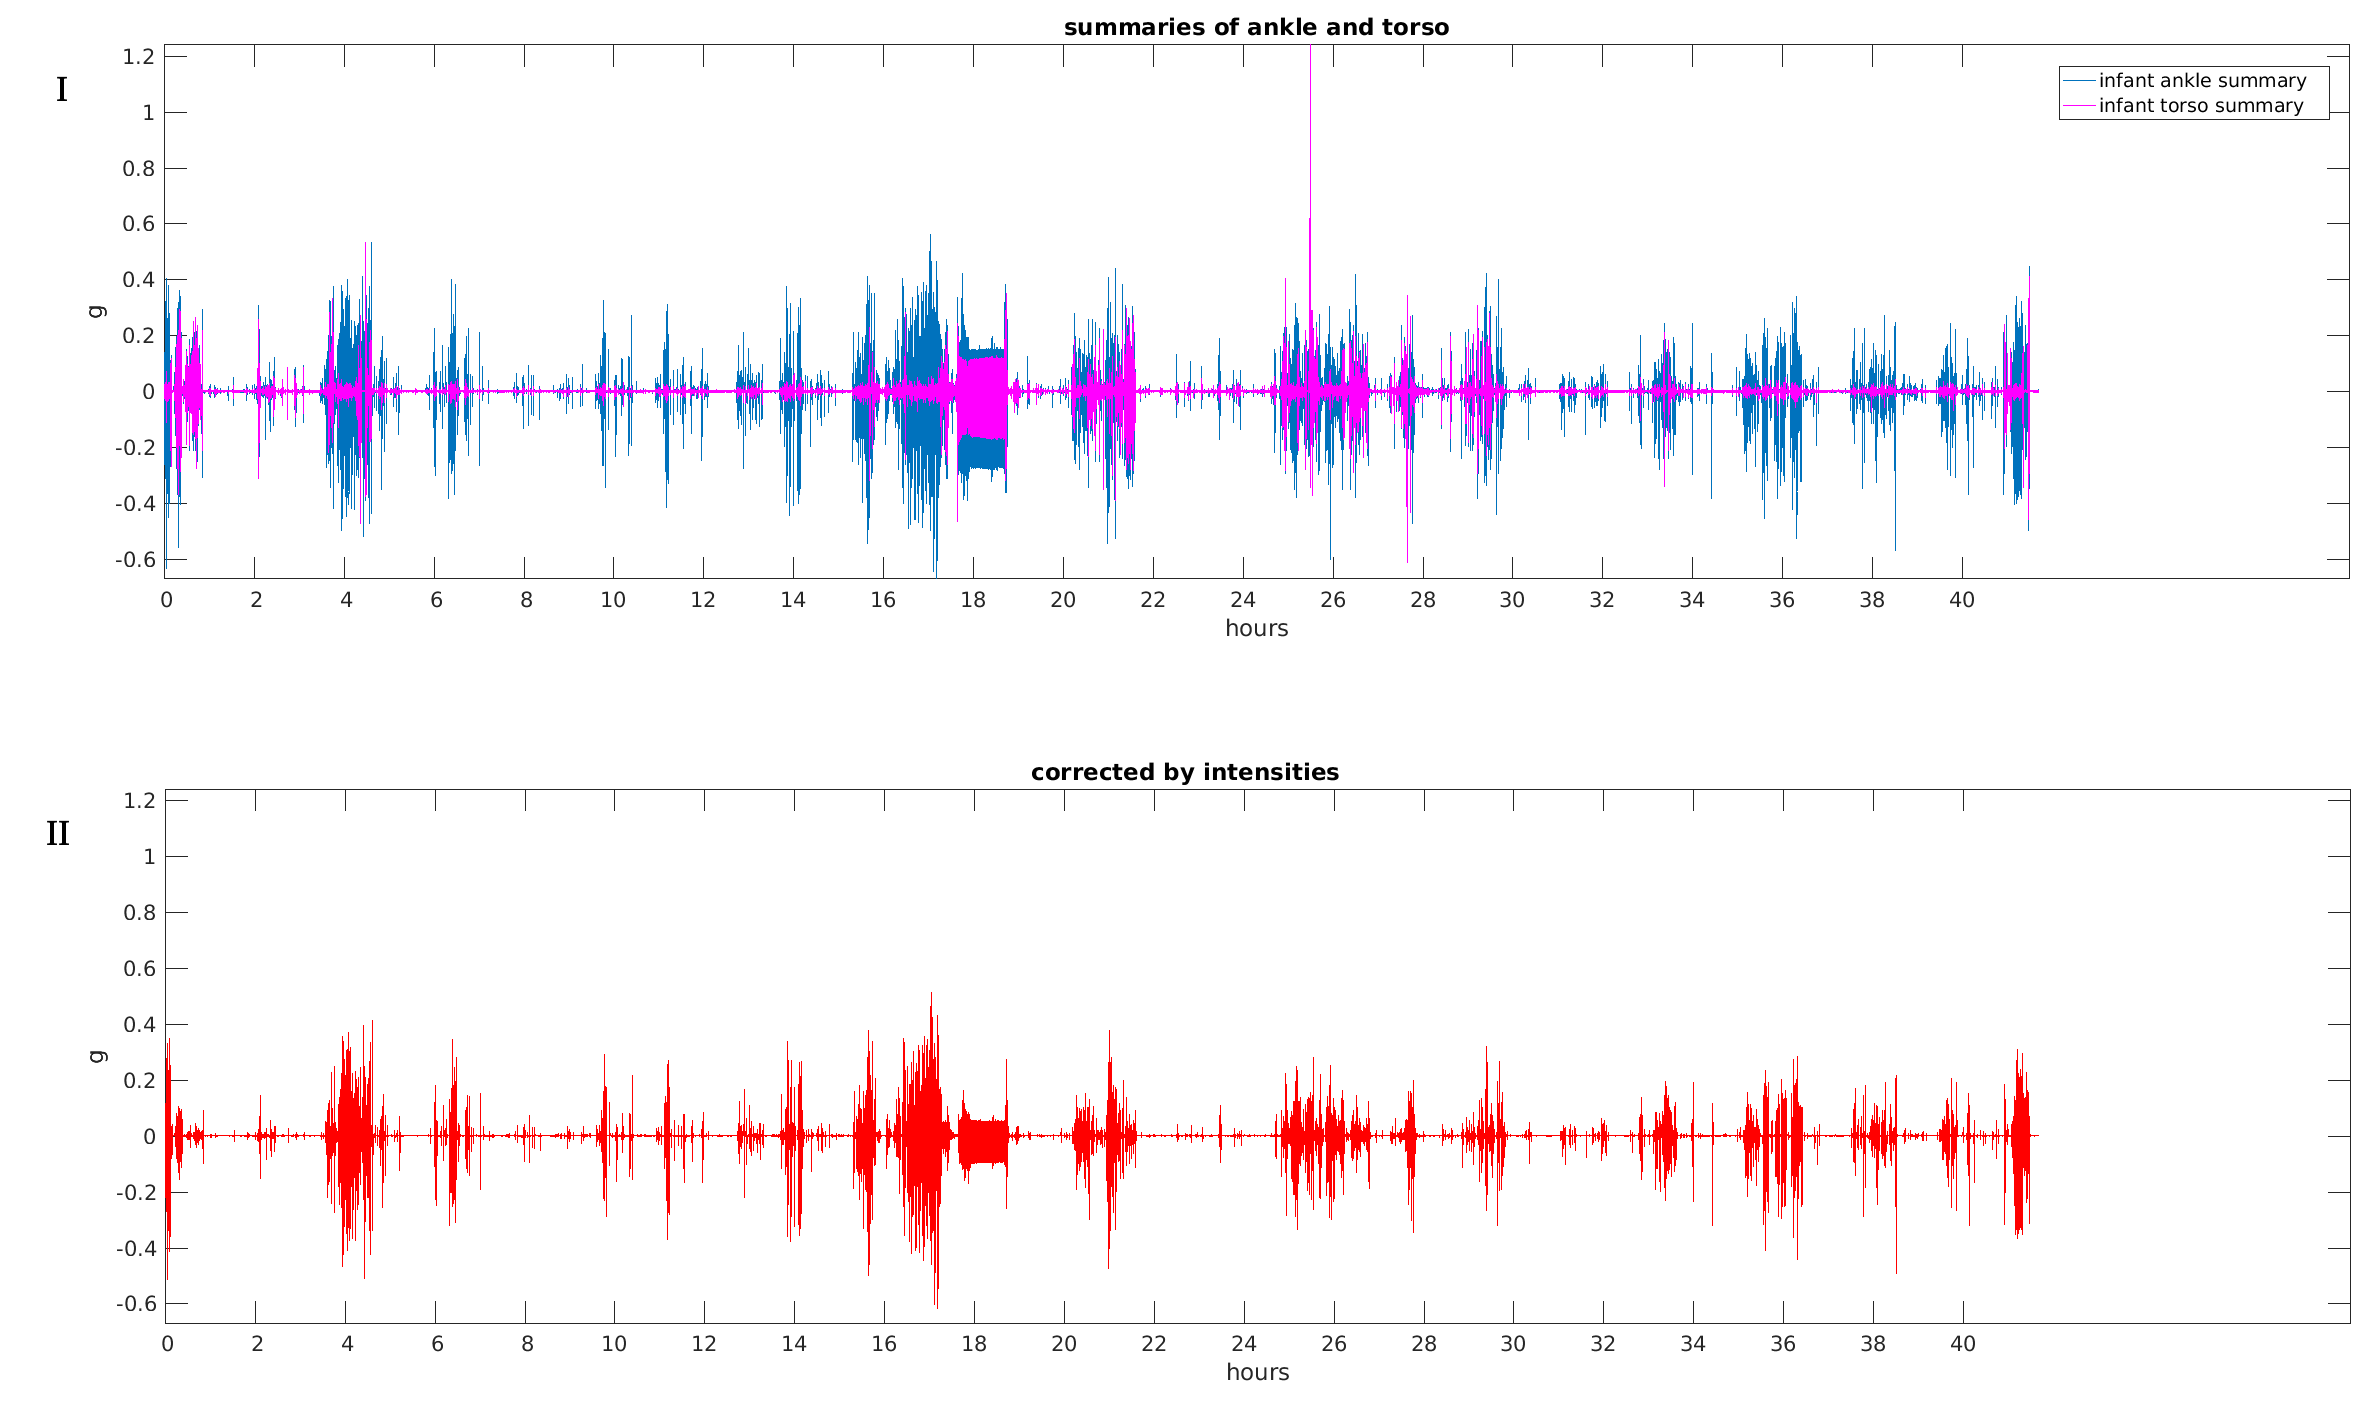
\includegraphics[width=15cm, height=7.5cm]{correctingIntensities.png}
\caption{A plot exhibiting the first summary derivations of the torso and ankle placed measurements (I) and the result (II) obtained by decreasing the accelerations in the first summary derivation of the ankle placed measurement by a factor equal to the ratio of the corresponding windowed absolute intensities.}
\end{figure}
\newpage
\begin{figure}[h!]
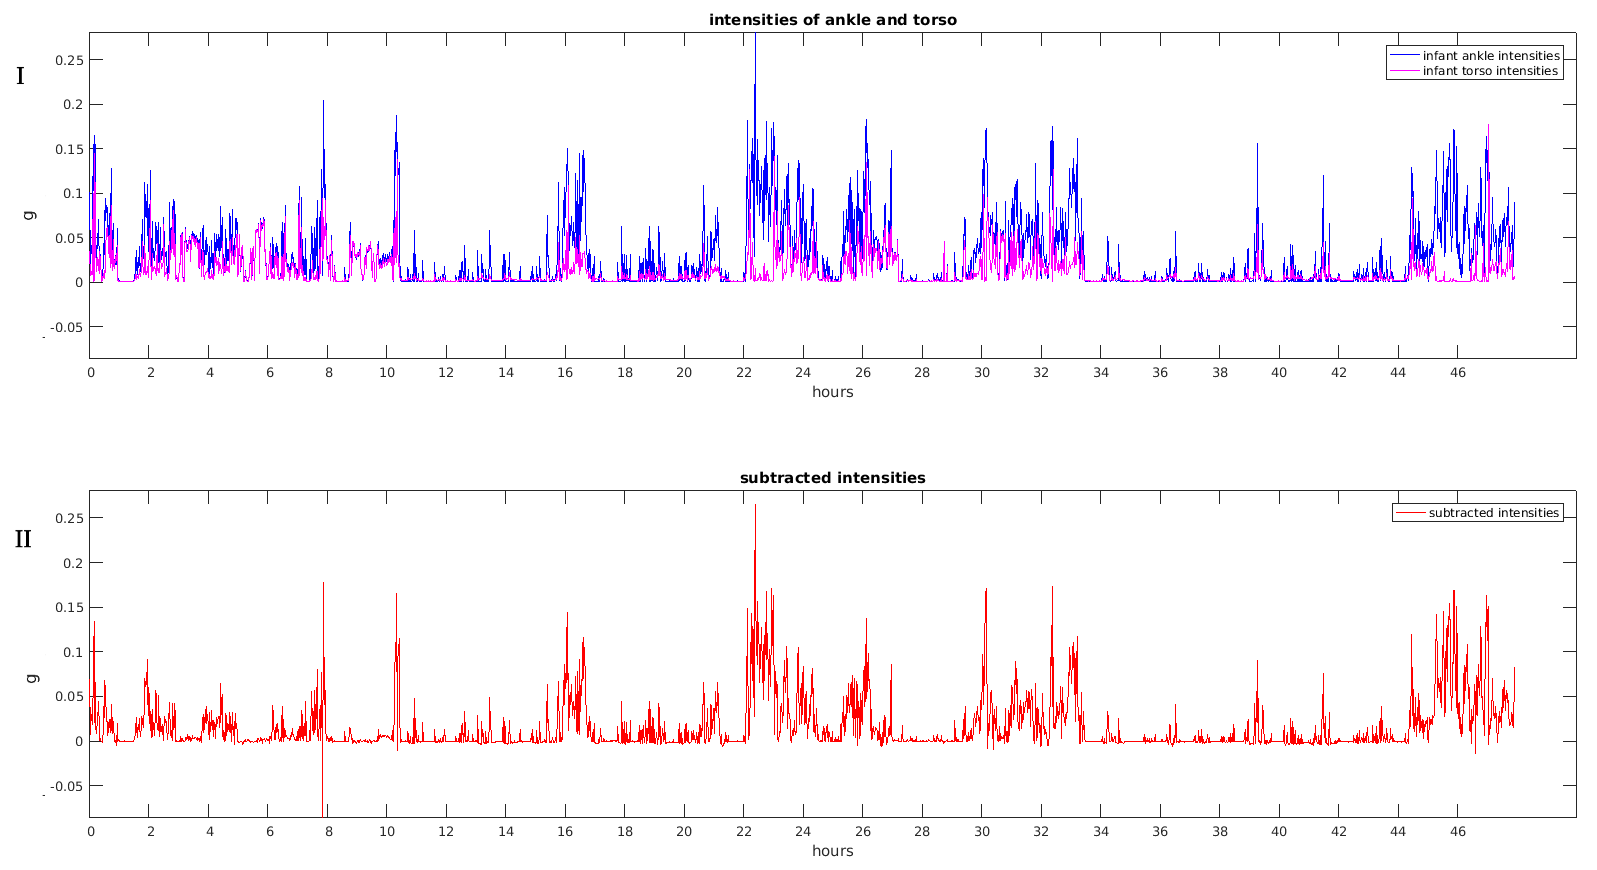
\includegraphics[width=15cm, height=8cm]{bandpass_summary_example_B.png}
\caption{An example of windowed absolute intensities obtained from the second summary derivations of torso and ankle placed measurements (I) and the result obtained by subtracting the windowed absolute intensities (II).}
\end{figure}
\begin{figure}[h!]
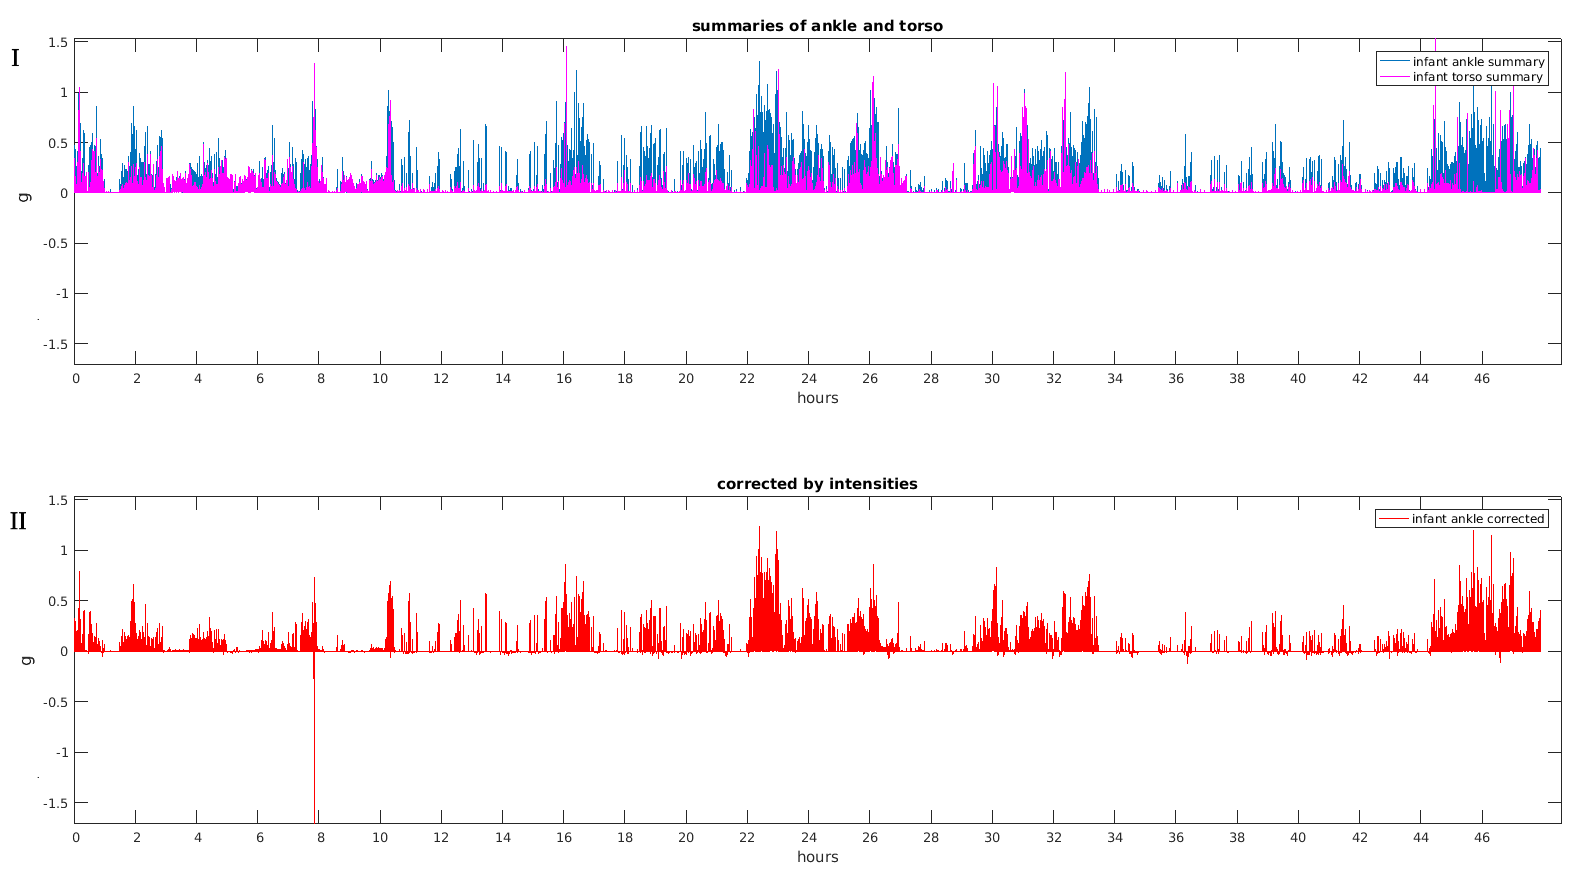
\includegraphics[width=15cm, height=8cm]{bandpass_summary_example_C.png}
\caption{A plot exhibiting the second summary derivations of the torso and ankle placed measurements (I) and the result (II) obtained by decreasing the accelerations in the second summary derivation of the ankle placed measurement by a factor equal to the ratio of the corresponding windowed absolute intensities.}
\end{figure}
\newpage
Although the accelerations on the ankle placed measurement are decreased in both approaches, the contributing accelerations are still clearly visible in both cases, while one can also observe negative absolute intensities due to the fact that the torso placed accelerometer can also record more intensive accelerations than the ankle placed one. Since it has been shown that the same activity performed by the caretaker is recorded differently by differently placed accelerometers, there should be a scaling factor involved when doing such subtractions or corrections. Obtaining such a scaling factor might be problematic, since it has also been shown that different activities result in different ratios between the differently placed accelerometers with high variability between the subjects \cite{ref5}. Things get even more complicated if considering the fact that the two accelerometers will also pick up additional accelerations, mainly infants own accelerations which are unique for that specific body part, like for example accelerations due to crying, flexing or kicking.\\Without having a well-defined training dataset it is difficult to tell which of the remaining accelerations after approaches \textbf{B} and \textbf{C} are due to excessive detection of contributing accelerations on the ankle placed accelerometer or due to infants PA. Nevertheless, the approaches can be improved.\\The concept of subtracting implies that the torso placed accelerometer will record accelerations equal or smaller then the ankle placed one, as well as that the degree of correction is dependent on the ratio of intensity instead of similarity. If similarity between the absolute intensities is obtained, it can be used as an approximation of the true scaling factor needed to accurately correct the ankle placed accelerometer. \\
In the approach \textbf{D}, an attempt is made to obtain signal similarities based on the similarity of windowed absolute intensities, using Pearsons correlation coefficient. The goal of the approach is to find similar patterns between the two measurements and then decrease the ankle placed measurement based on the degree of similarity. The idea behind this is that even though the two differently placed accelerometers might record the same activity different, there should be an underlying pattern in both, at least on a large enough window scale over the absolute intensities. For example some periods might exhibit similarity only in the global changes as shown in Figure 12, while others might be more similar even on the local scale as shown in Figure 13.
\newpage
\begin{figure}[h!]
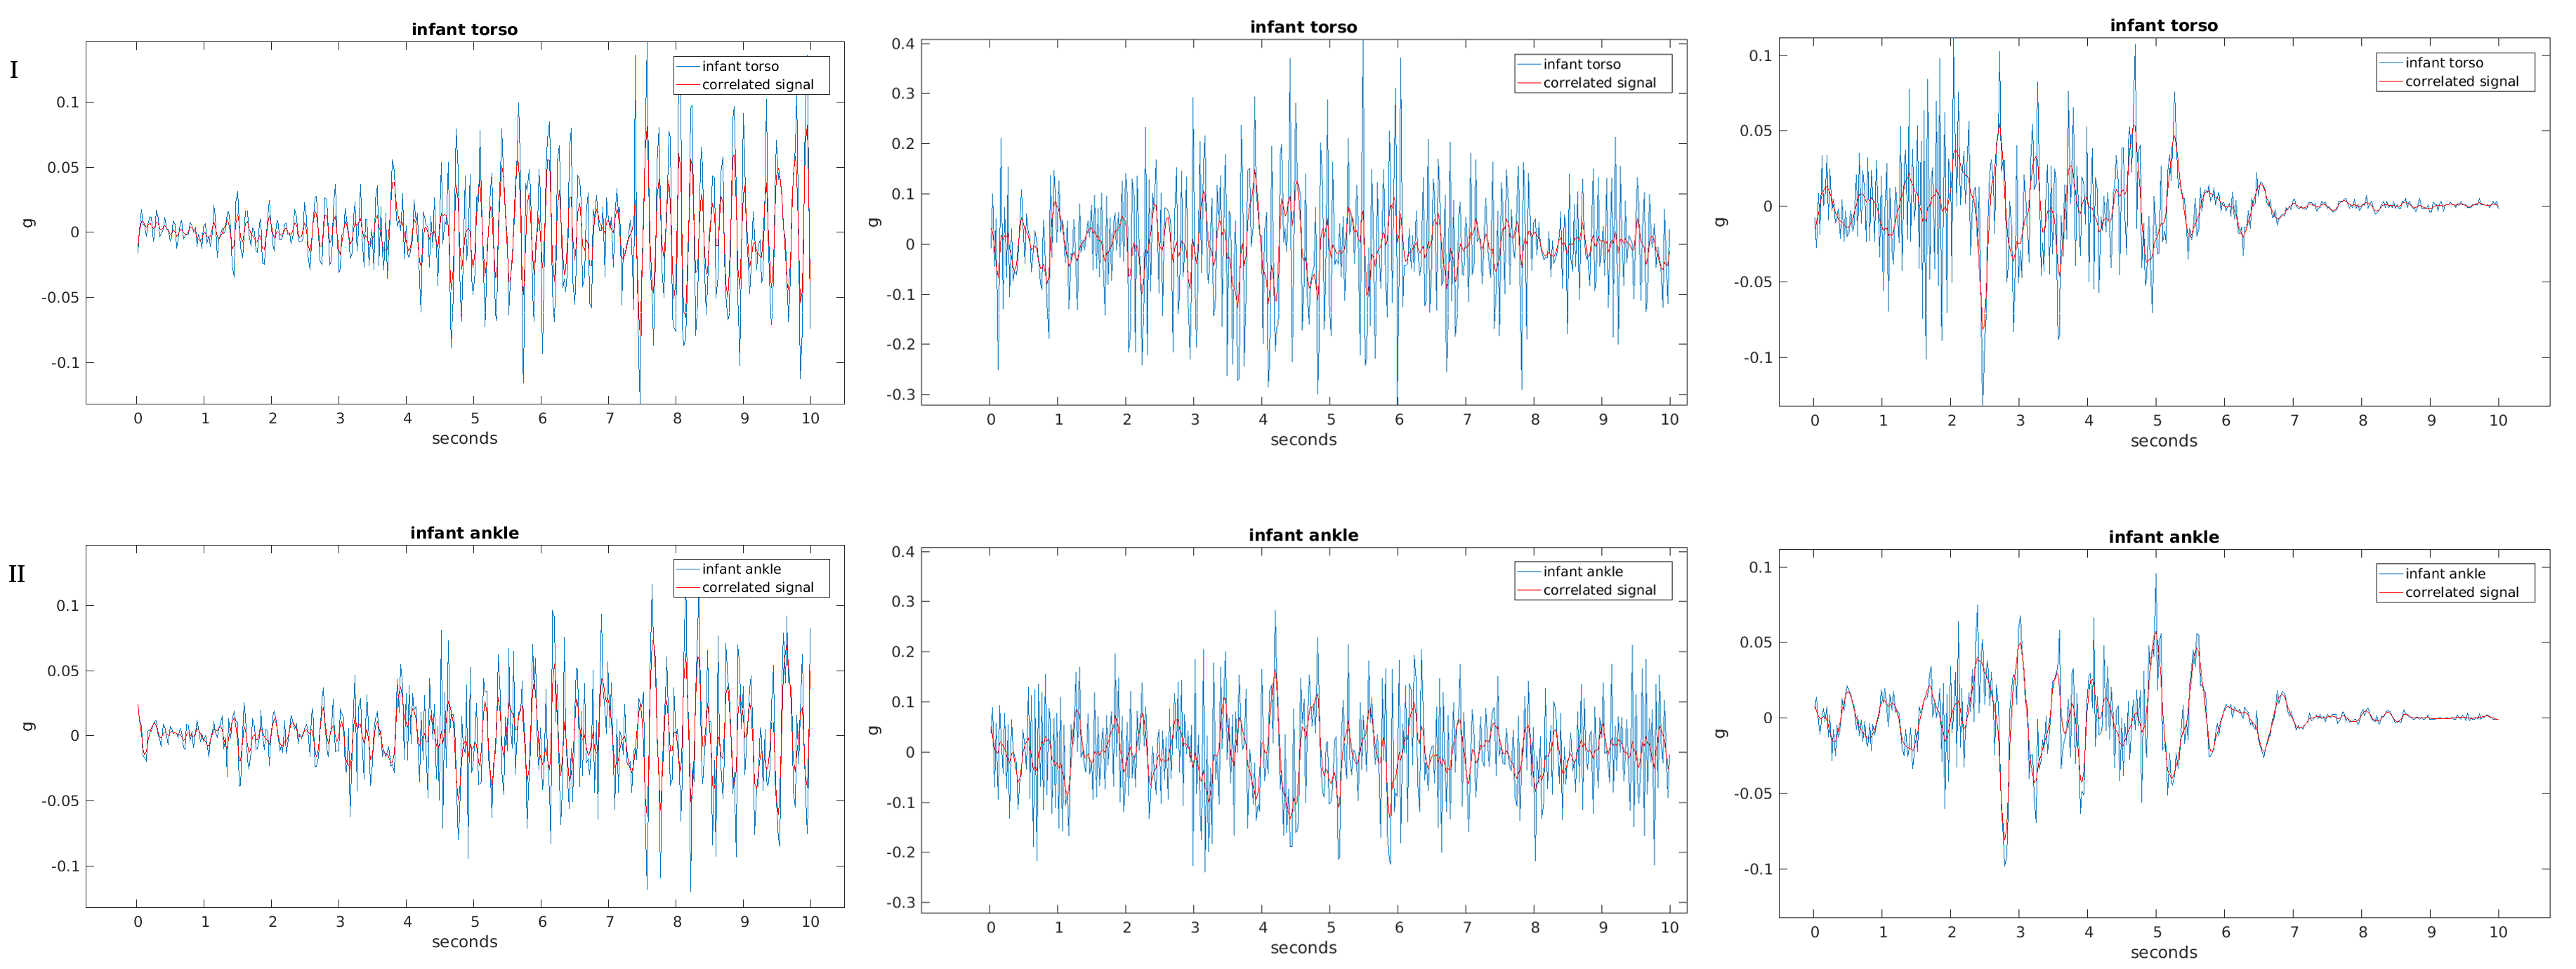
\includegraphics[width=15cm, height=8cm]{roughSimilar.png}
\caption{A plot showing a few examples of similarities between the first summary derivations of the torso (I) and ankle (II) placed measurement on a global scale.}
\end{figure}
\begin{figure}[h!]
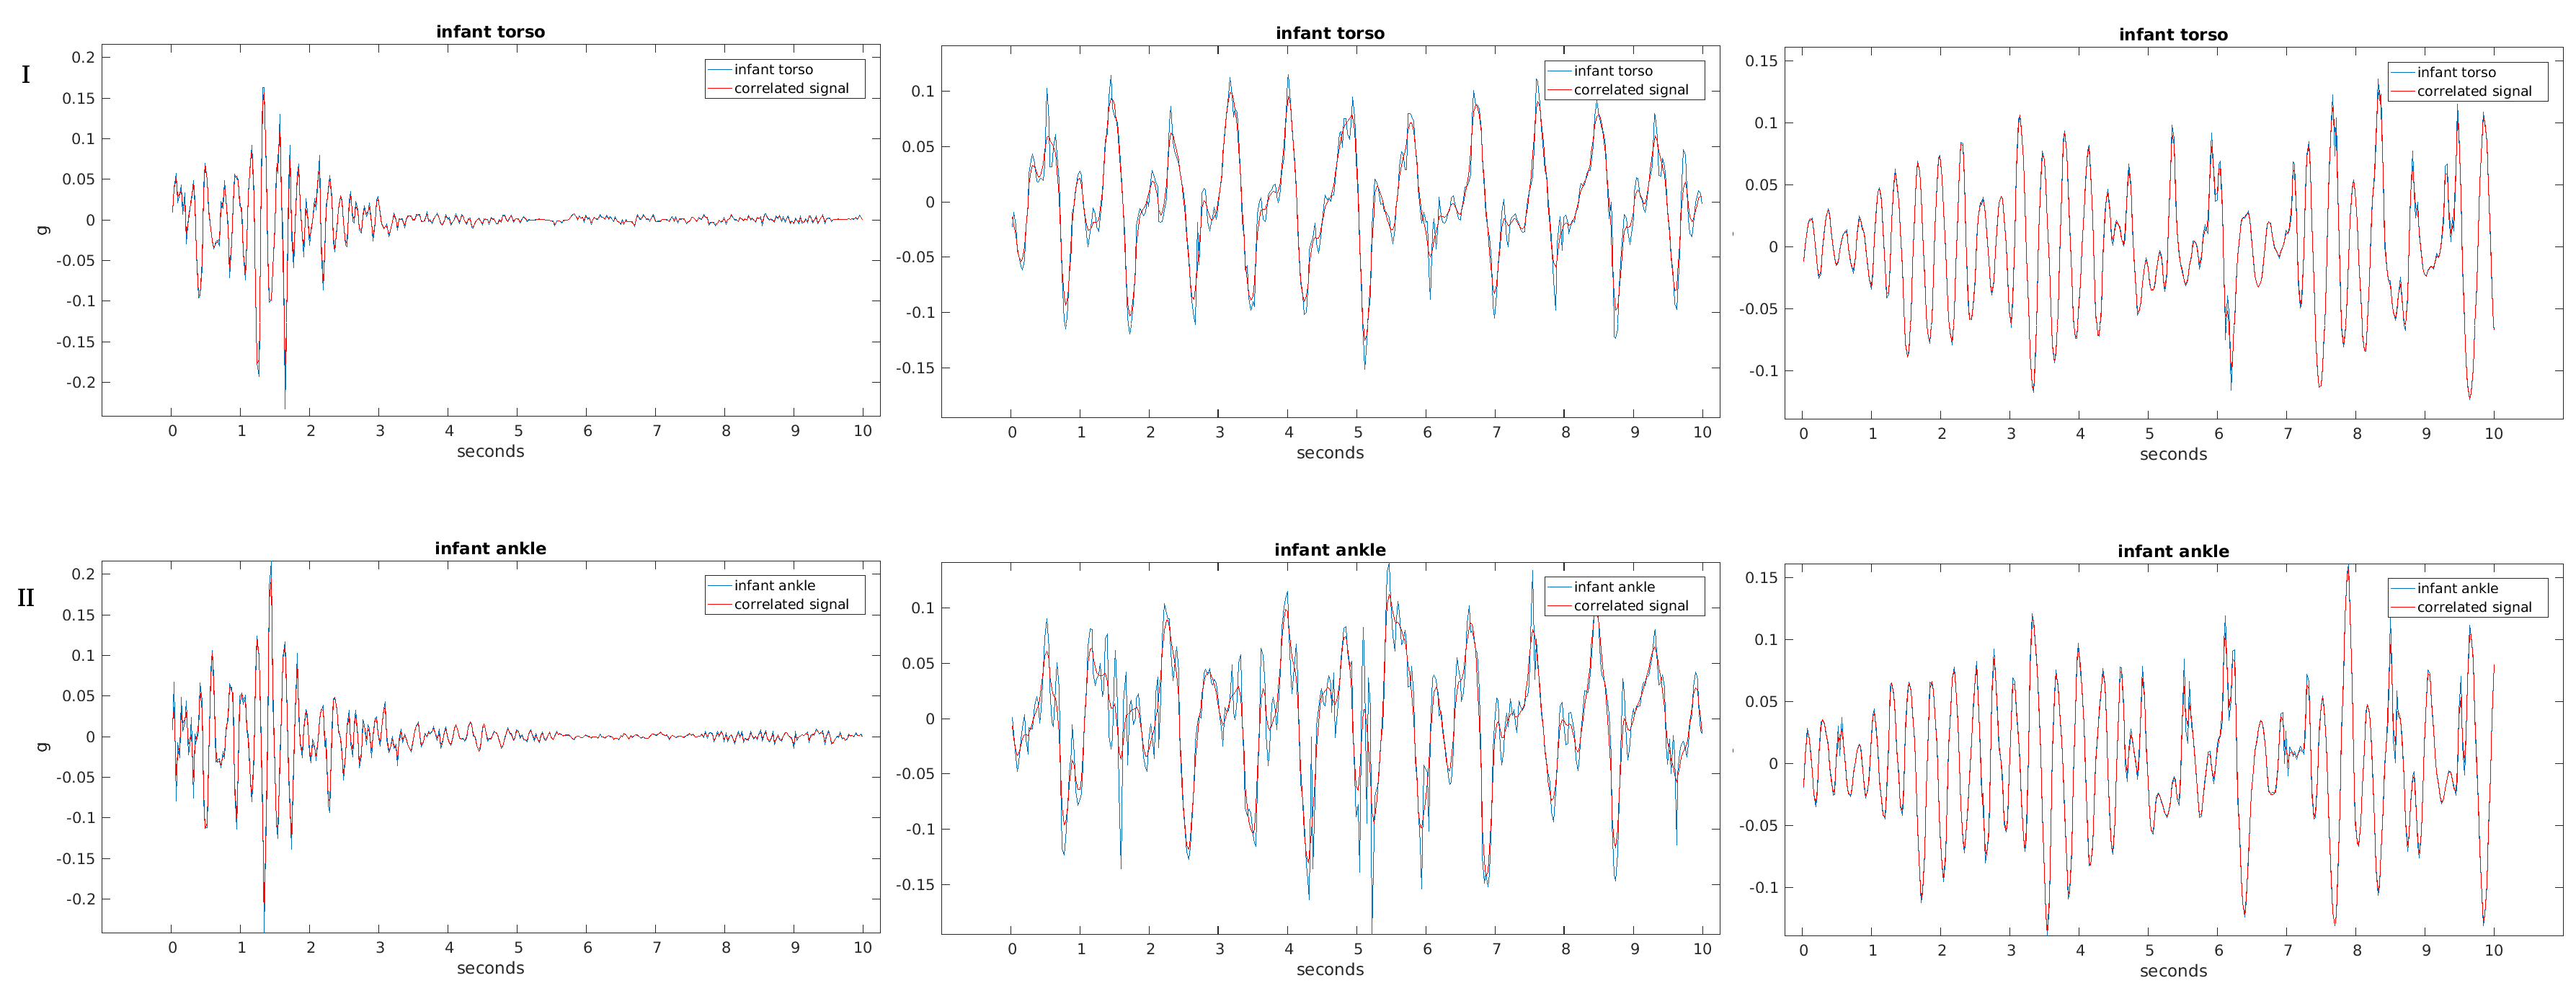
\includegraphics[width=15cm, height=8cm]{localSimilar.png}
\caption{A plot showing a few examples of more precise similarities between the first summary derivations of the torso (I) and ankle (II) placed measurement on a local scale.}
\end{figure}
\newpage
The main issue with previous approaches \textbf{A}, \textbf{B} and \textbf{C} are the local point to point differences between the two differently placed accelerometers recording the same activity. These differences are characterized by larger accelerations on one of the accelerometers, presence of previously mentioned additional accelerations or noise in one or both measurements or in a form a time lag, examples shown in Figure 14.
Taking these differences into account, we would still like to determine if the two measurements in a given window are changing together due to being under the influence of the same activity, which is why calculating their covariance is of interest. Pearson correlation is obtained by dividing the covariance of the two variables by the product of their standard deviations and is a common correlation used for comparing signal similarities, especially in alignment\cite{ref9}. The fact that it is invariant to separate changes in location and scale in the two variables being compared, gives it potential to expose the underlying similarities of the two differently placed accelerometers.
\begin{figure}[h]
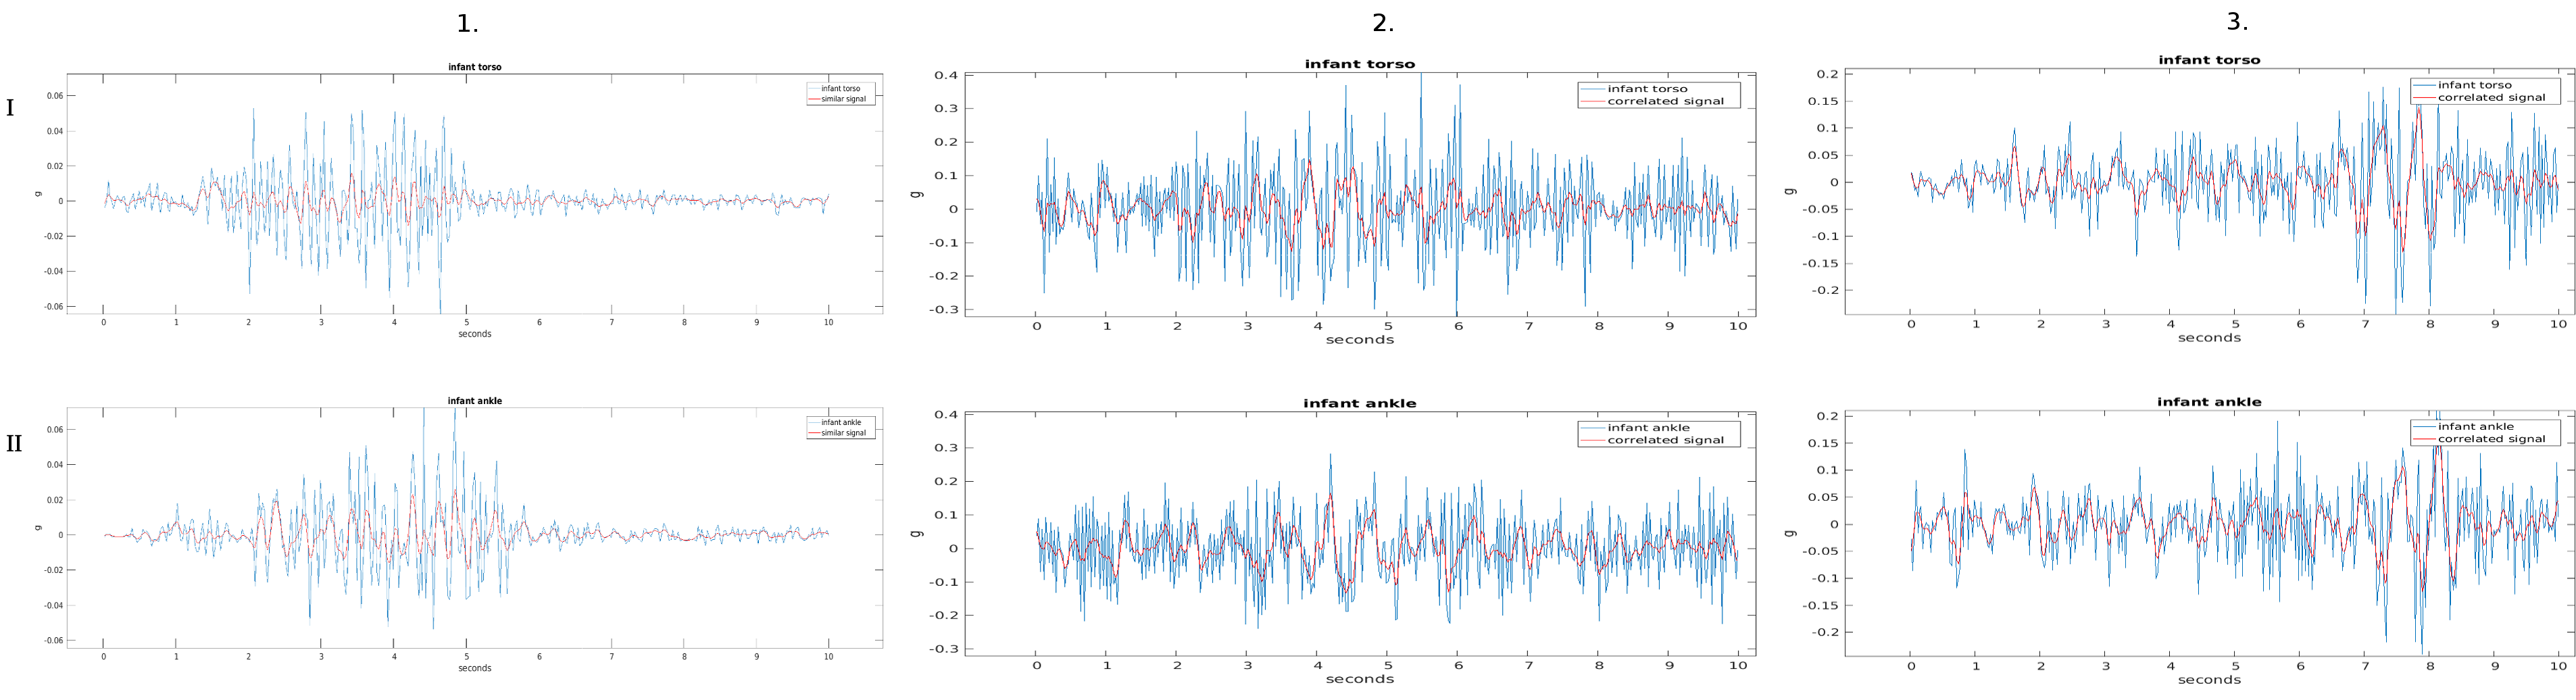
\includegraphics[width=15cm, height=6.5cm]{differences.png}
\caption{First (1.) plot showing a slight time lag between the torso (I) and the ankle (II) placed measurement, second (2.) plot showing larger accelerations on the torso (I) placed accelerometer and the third (3.) plot showing the presence of additional accelerations and noise in both torso (I) and ankle (II) placed measurements.}
\end{figure}\\

Nevertheless, large differences, previously mentioned additional accelerations and time lags can still influence the correlation coefficient. Even though Figure 8 and 9 exhibit similar patterns in the derived summaries of the torso and ankle placed measurement, the overall proportion of windows, where the absolute correlation coefficient is large enough and significant, turns out to be very small. To get the desired results in approach \textbf{D}, further summarization is required in a form of windowed absolute intensities, as in approaches \textbf{B} and \textbf{C}.\\ 
Approach \textbf{D} is also implemented in Matlab. Absolute intensities are calculated for windows of 200 points, which corresponds to 5 seconds. Correlation coefficient is obtained with the build-in Matlab function \textit{corr}, for windows of 24 windowed absolute intensities, which corresponds to total 2 minutes, sliding with a step size 12, which corresponds to 1 minute. P-value is obtained using the permutation test with 10 repetitions. If p-value is non-significant, correlation coefficient is set to 0. While sliding, the first half will overlap with the previous window. Therefor, previous correlation coefficient is compared with the current and the biggest is used as a factor to decrease the first half of the corresponding window of the original derived summary of the ankle placed measurement, while the second half is decreased with a factor equal to the current absolute correlation coefficient. The final result is the original summary derivation of the ankle placed measurement, where windowed accelerations are decreased by the factor equal to the absolute correlation coefficient of windowed absolute intensities. Figure 15 shows an example of the first summary derivations of torso and ankle placed measurements and the corresponding result from approach \textbf{D}, along with the corresponding result from approach \textbf{C}, to enable comparison. Figure 16 shows an example of the second summary derivations of torso and ankle placed measurements and the corresponding result from approach \textbf{D}, along with the corresponding result from approach \textbf{C}, to enable comparison.

\begin{figure}[h!]
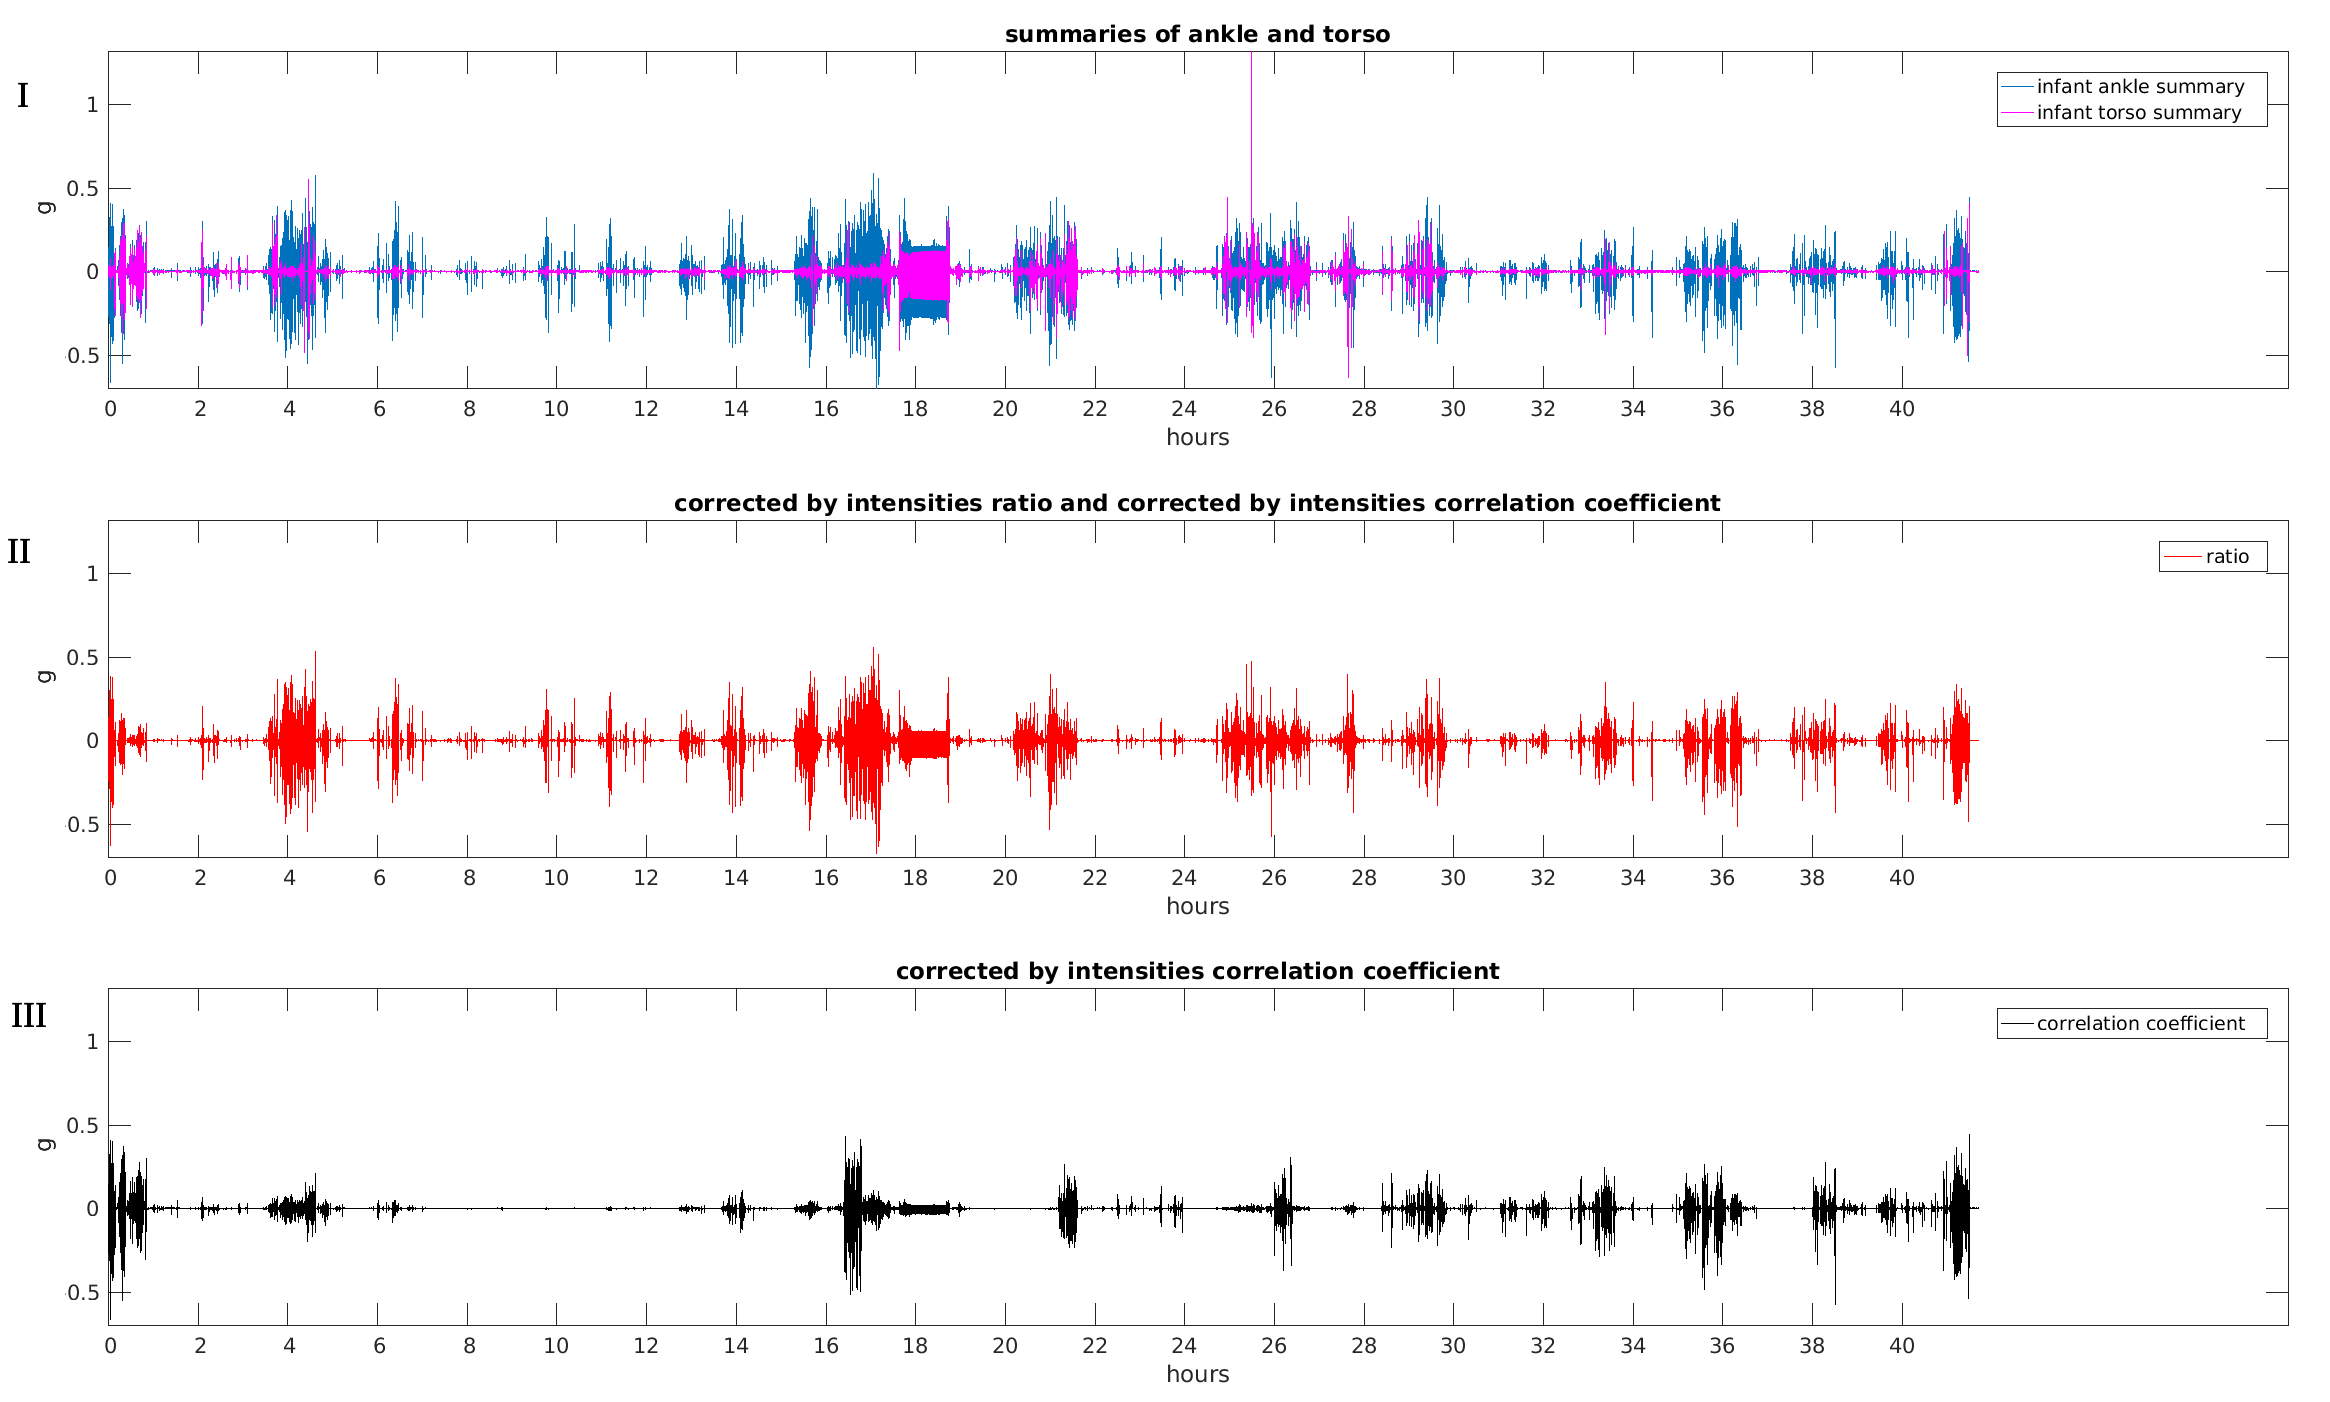
\includegraphics[width=15cm, height=8cm]{CorrectedIntensitiesCorrelation_result.png}
\caption{A plot exhibiting the first summary derivations of the torso and ankle placed measurements (I) and the different results from approach \textbf{C} (II) and \textbf{D} (III). One can see substantially less left-overs from the contributing accelerations in the approach \textbf{D}.}
\end{figure}

\begin{figure}[h!]
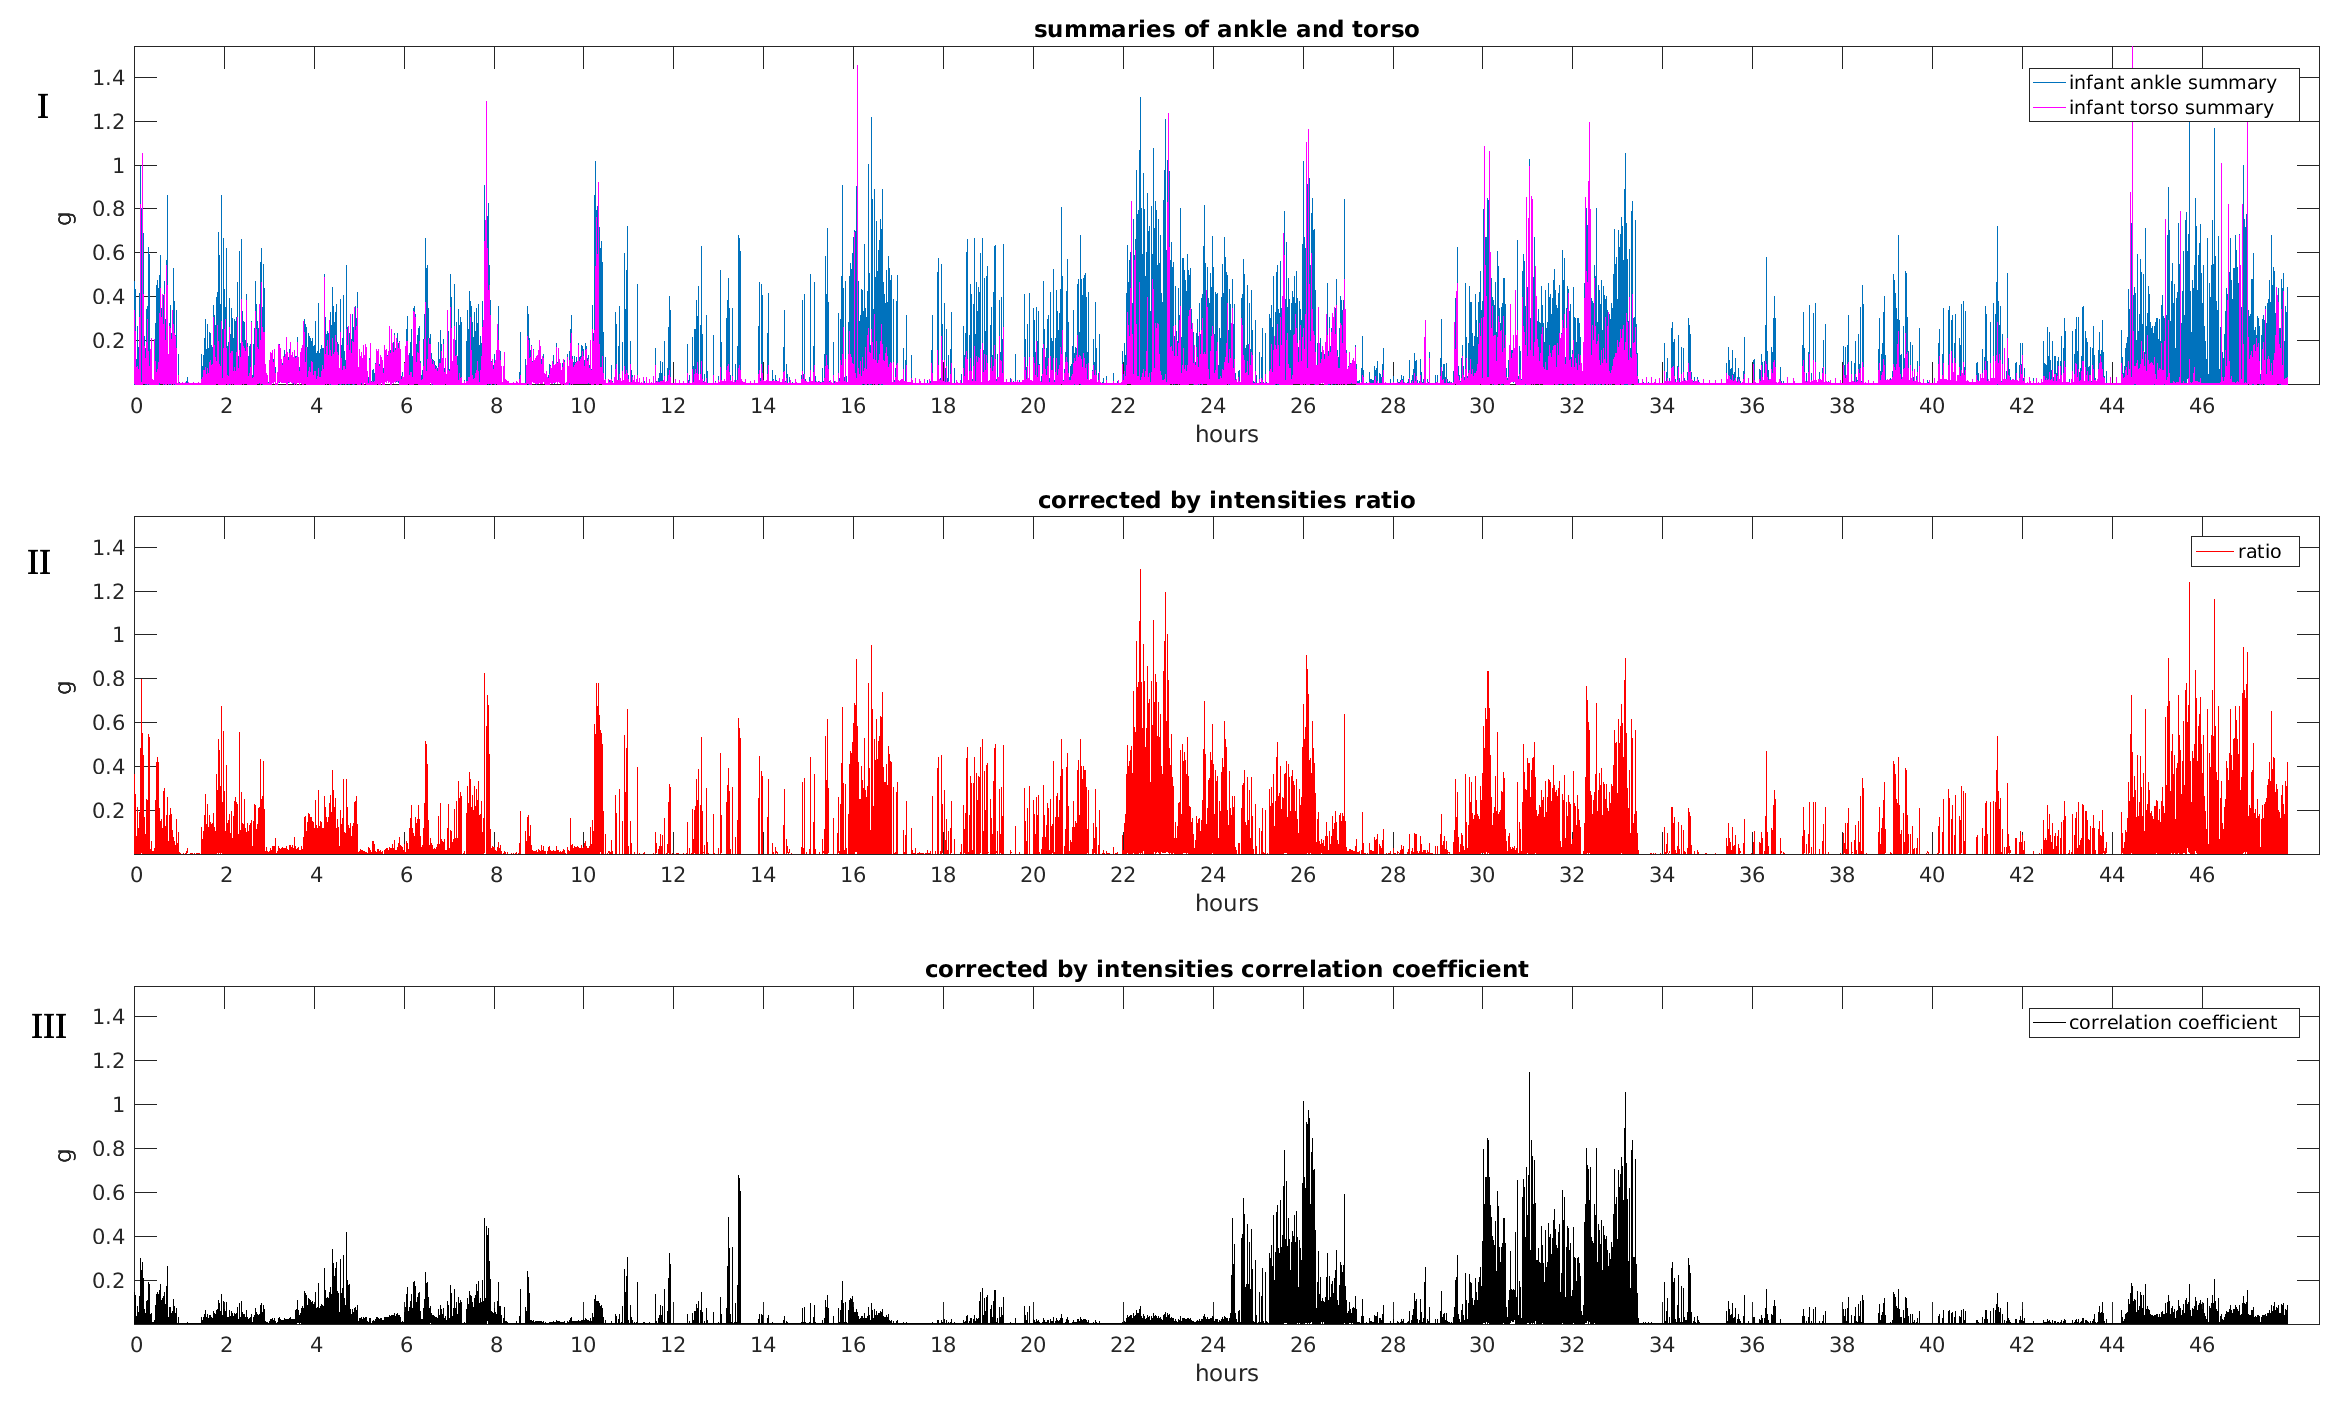
\includegraphics[width=15cm, height=8cm]{approachD_second_summary.png}
\caption{A plot exhibiting the second summary derivations of the torso and ankle placed measurements (I) and the different results from approach \textbf{C} (II) and \textbf{D} (III). One can see substantially less left-overs from the contributing accelerations in the approach \textbf{D}.}
\end{figure}
\\
\newpage
Although there are less visible left-overs of contributing accelerations after the approach \textbf{D}, there are still there and one would like to extract PA from a measurement that does not include any contributing accelerations.
For that purpose, in approach \textit{E}, periods where SD is increased in both, torso and ankle placed measurement, are extracted and removed, allowing only periods where large acceleration can only occur on the ankle placed measurement. The extracted periods approximate periods when the infant was being moved, by removing these periods, the following PA extraction should result in PA levels represented by the infants activity only. \\Periods when the infant was being moved are extracted similar as in non-wear detection, based on a threshold for SD of accelerations in periods of fifteen seconds. In other words, the periods when the SD of accelerations on both, torso and ankle placed measurements are above that threshold, the period is assumed to be a period when the infant was being moved. Different outcomes are observed based on several different values of the threshold. If the two summary derivations are significantly different and have a different amount of variance, then the threshold for increased SD due to being moved should be set accordingly for each type. Analysis will reveal how different are the two types of summary derivation and whether they have a different amount of variance.\\
Nevertheless, upon trial of different thresholds and the examination of the final total proportion of time the infant is detected as being moved, different outcomes are observed for the two types of summary derivation when using the same threshold. At the same time, observations showed that the final proportion of data removed due to increased SD in both, torso and ankle placed measurements is quite high and dominant during the day, giving an impression as if only periods when the infant is sleeping remain. Therefor the threshold for SD of acceleration should be set carefully in order to best separate the periods when the infant is being moved and the periods when only the infant himself is active. Observations mentioned above are taken into consideration when doing further analysis, so that the most appropriate values for the threshold are set for each type of the summary derivation. Example of the obtained periods, when the infant is detected to be moved, for the first summary derivation, when setting the threshold value for SD of accelerations to 0.006 g, shown in Figure 17.
\begin{figure}[h]
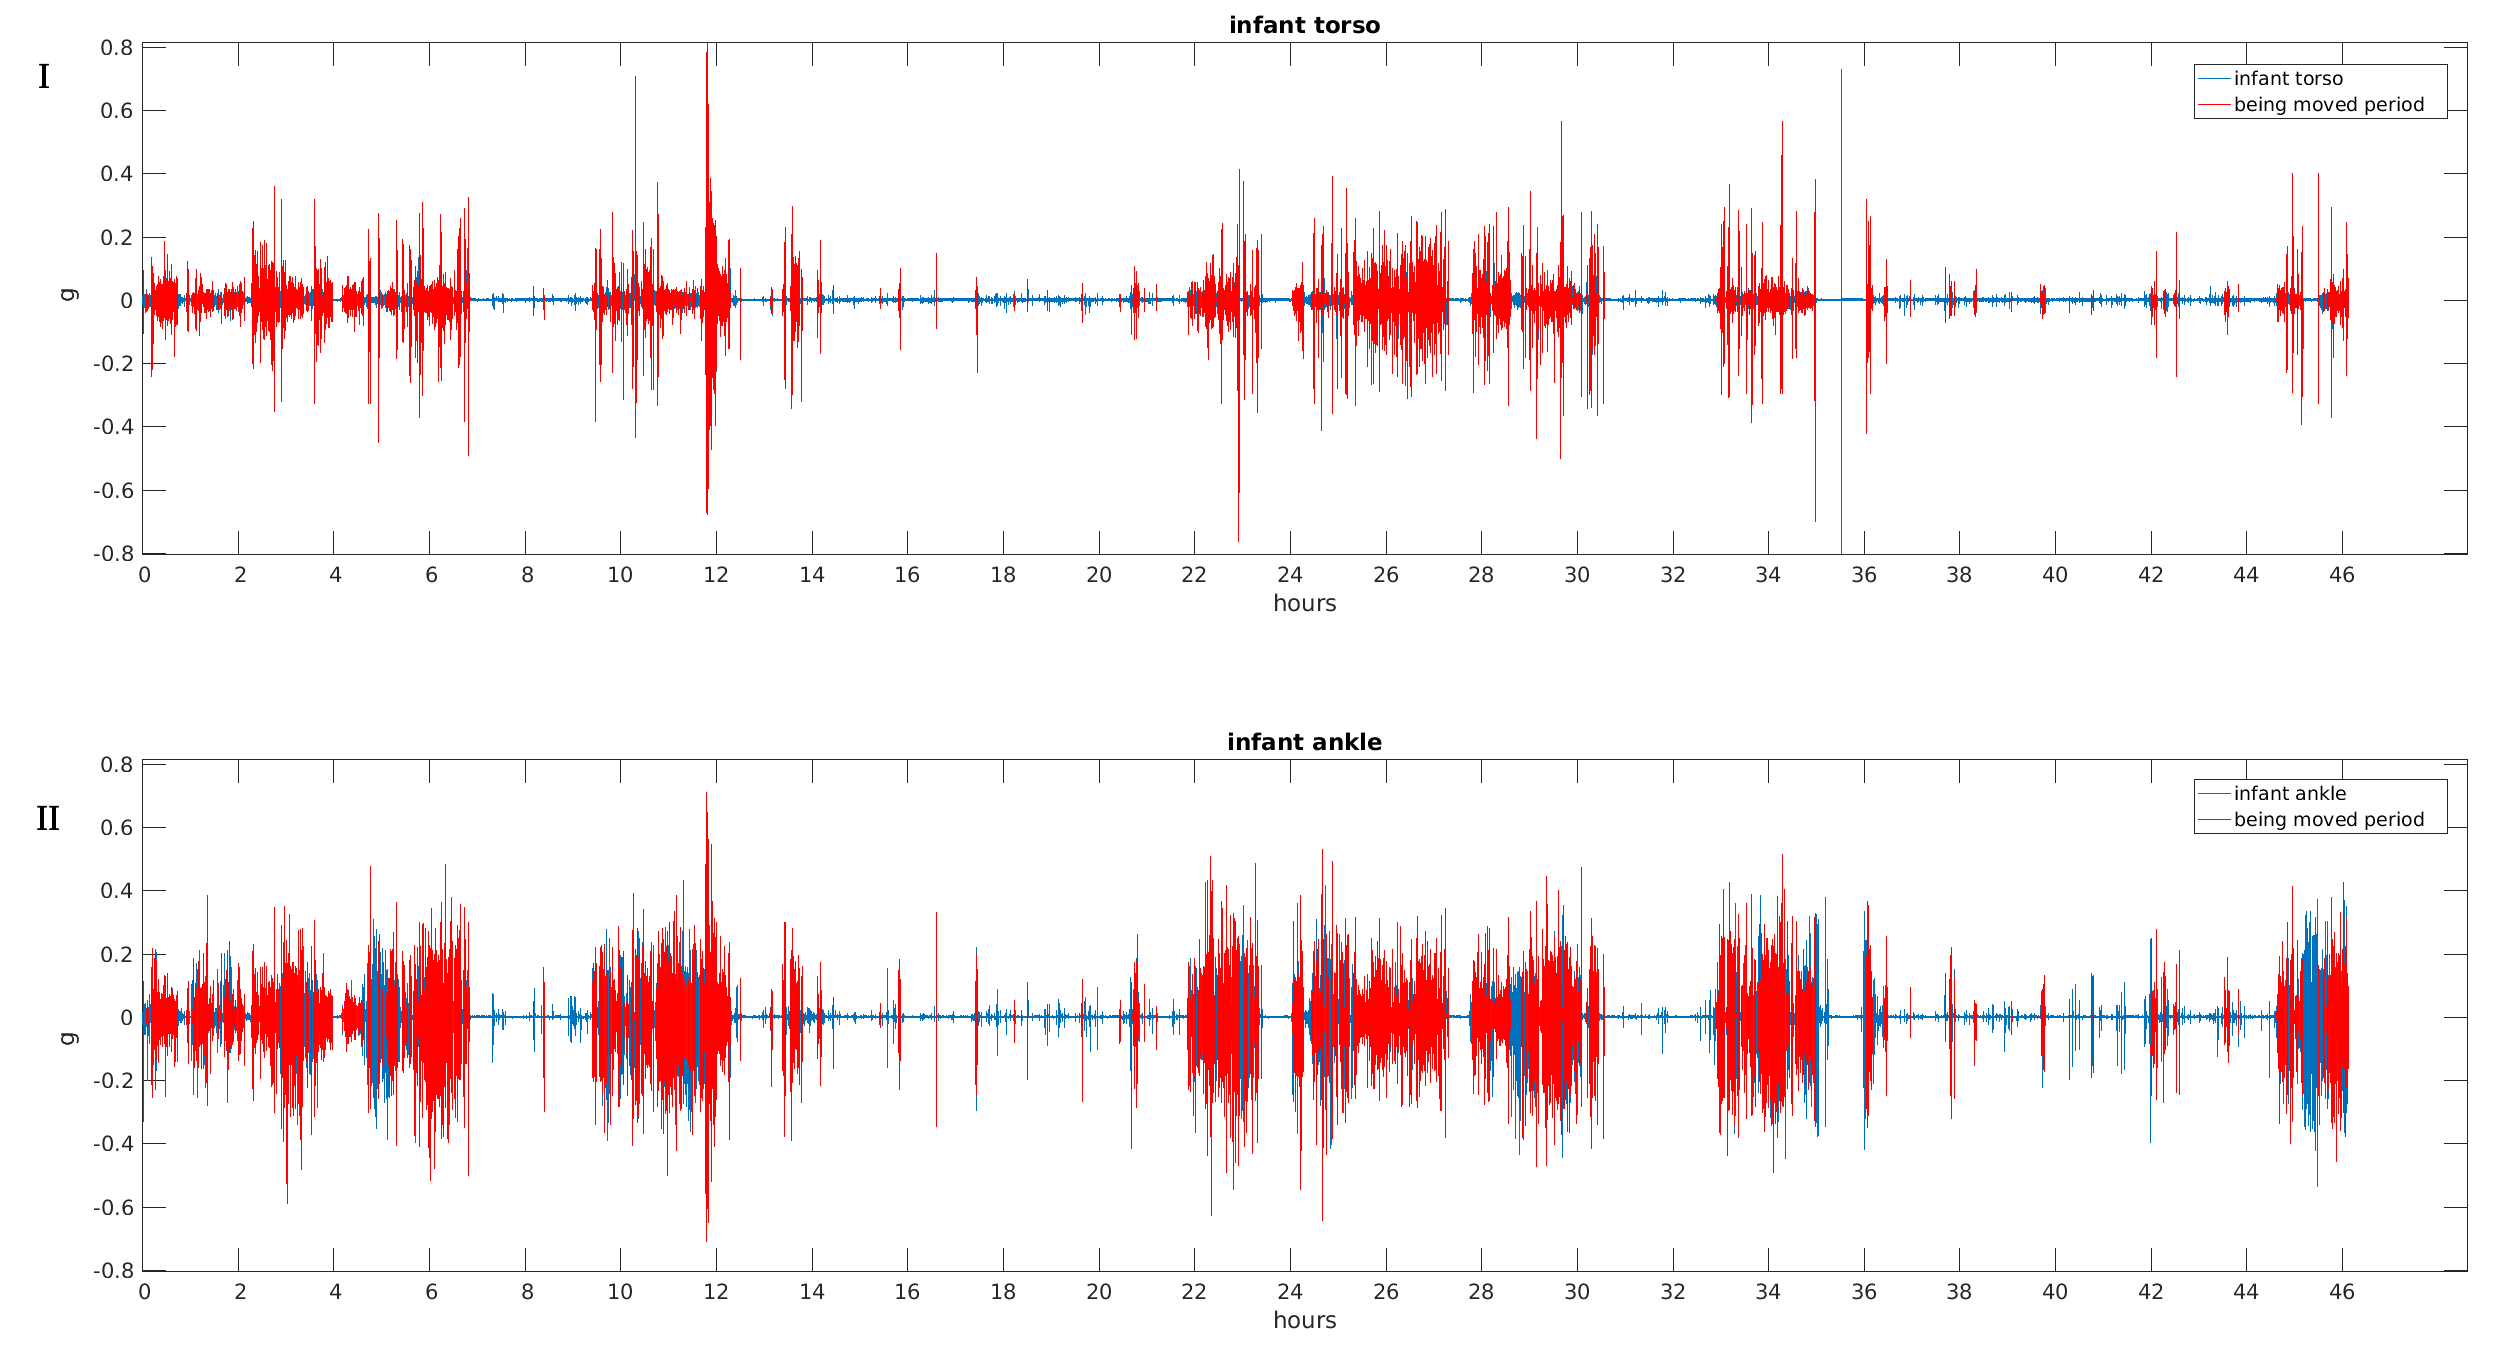
\includegraphics[width=15cm, height=8cm]{example_approach_E.png}
\caption{Example of the first summary derivations of the torso (I) and ankle (II) placed measurements, where periods when the infant was being moved are highlighted in red.}
\end{figure}
\\Each approach results in an ankle placed measurement, where the caretakers contributed accelerations are attempted to be removed. Those results are used for PA extraction, where further comparison and assessment of the different approaches can be made.
\newpage
\subsection{Physical activity extraction}
PA is extracted from the corrected or remaining measurements, after removal of data points of non-wear time, summary derivation, correction for the gravitational component and the correction for caretakers contributing accelerations. In approaches where the result of the correction for caretakers contributing accelerations is in the form of the original summary, PA is extracted based on the increased SD in a windowed measurement, while in the approaches where the result of the correction for caretakers contributing accelerations is in a form of windowed absolute intensities, PA is extracted based on the increased intensities. Window size is set to 400 data points, which corresponds to 10 seconds and the step size is set to 40 data points, which corresponds to one second. Similar as in the extraction of periods when the infant was moved, the periods when the infant was active are extracted by setting the most appropriate threshold for each of the two types of summary derivation. Examples of periods when the infant was active, setting the threshold for SD to 0.005 g, based on the first summary derivation and caretakers contributions corrected with approach B, approach C, approach D or approach E shown in Figures 18, 19, 20 and 21, respectively.
\begin{figure}[h]
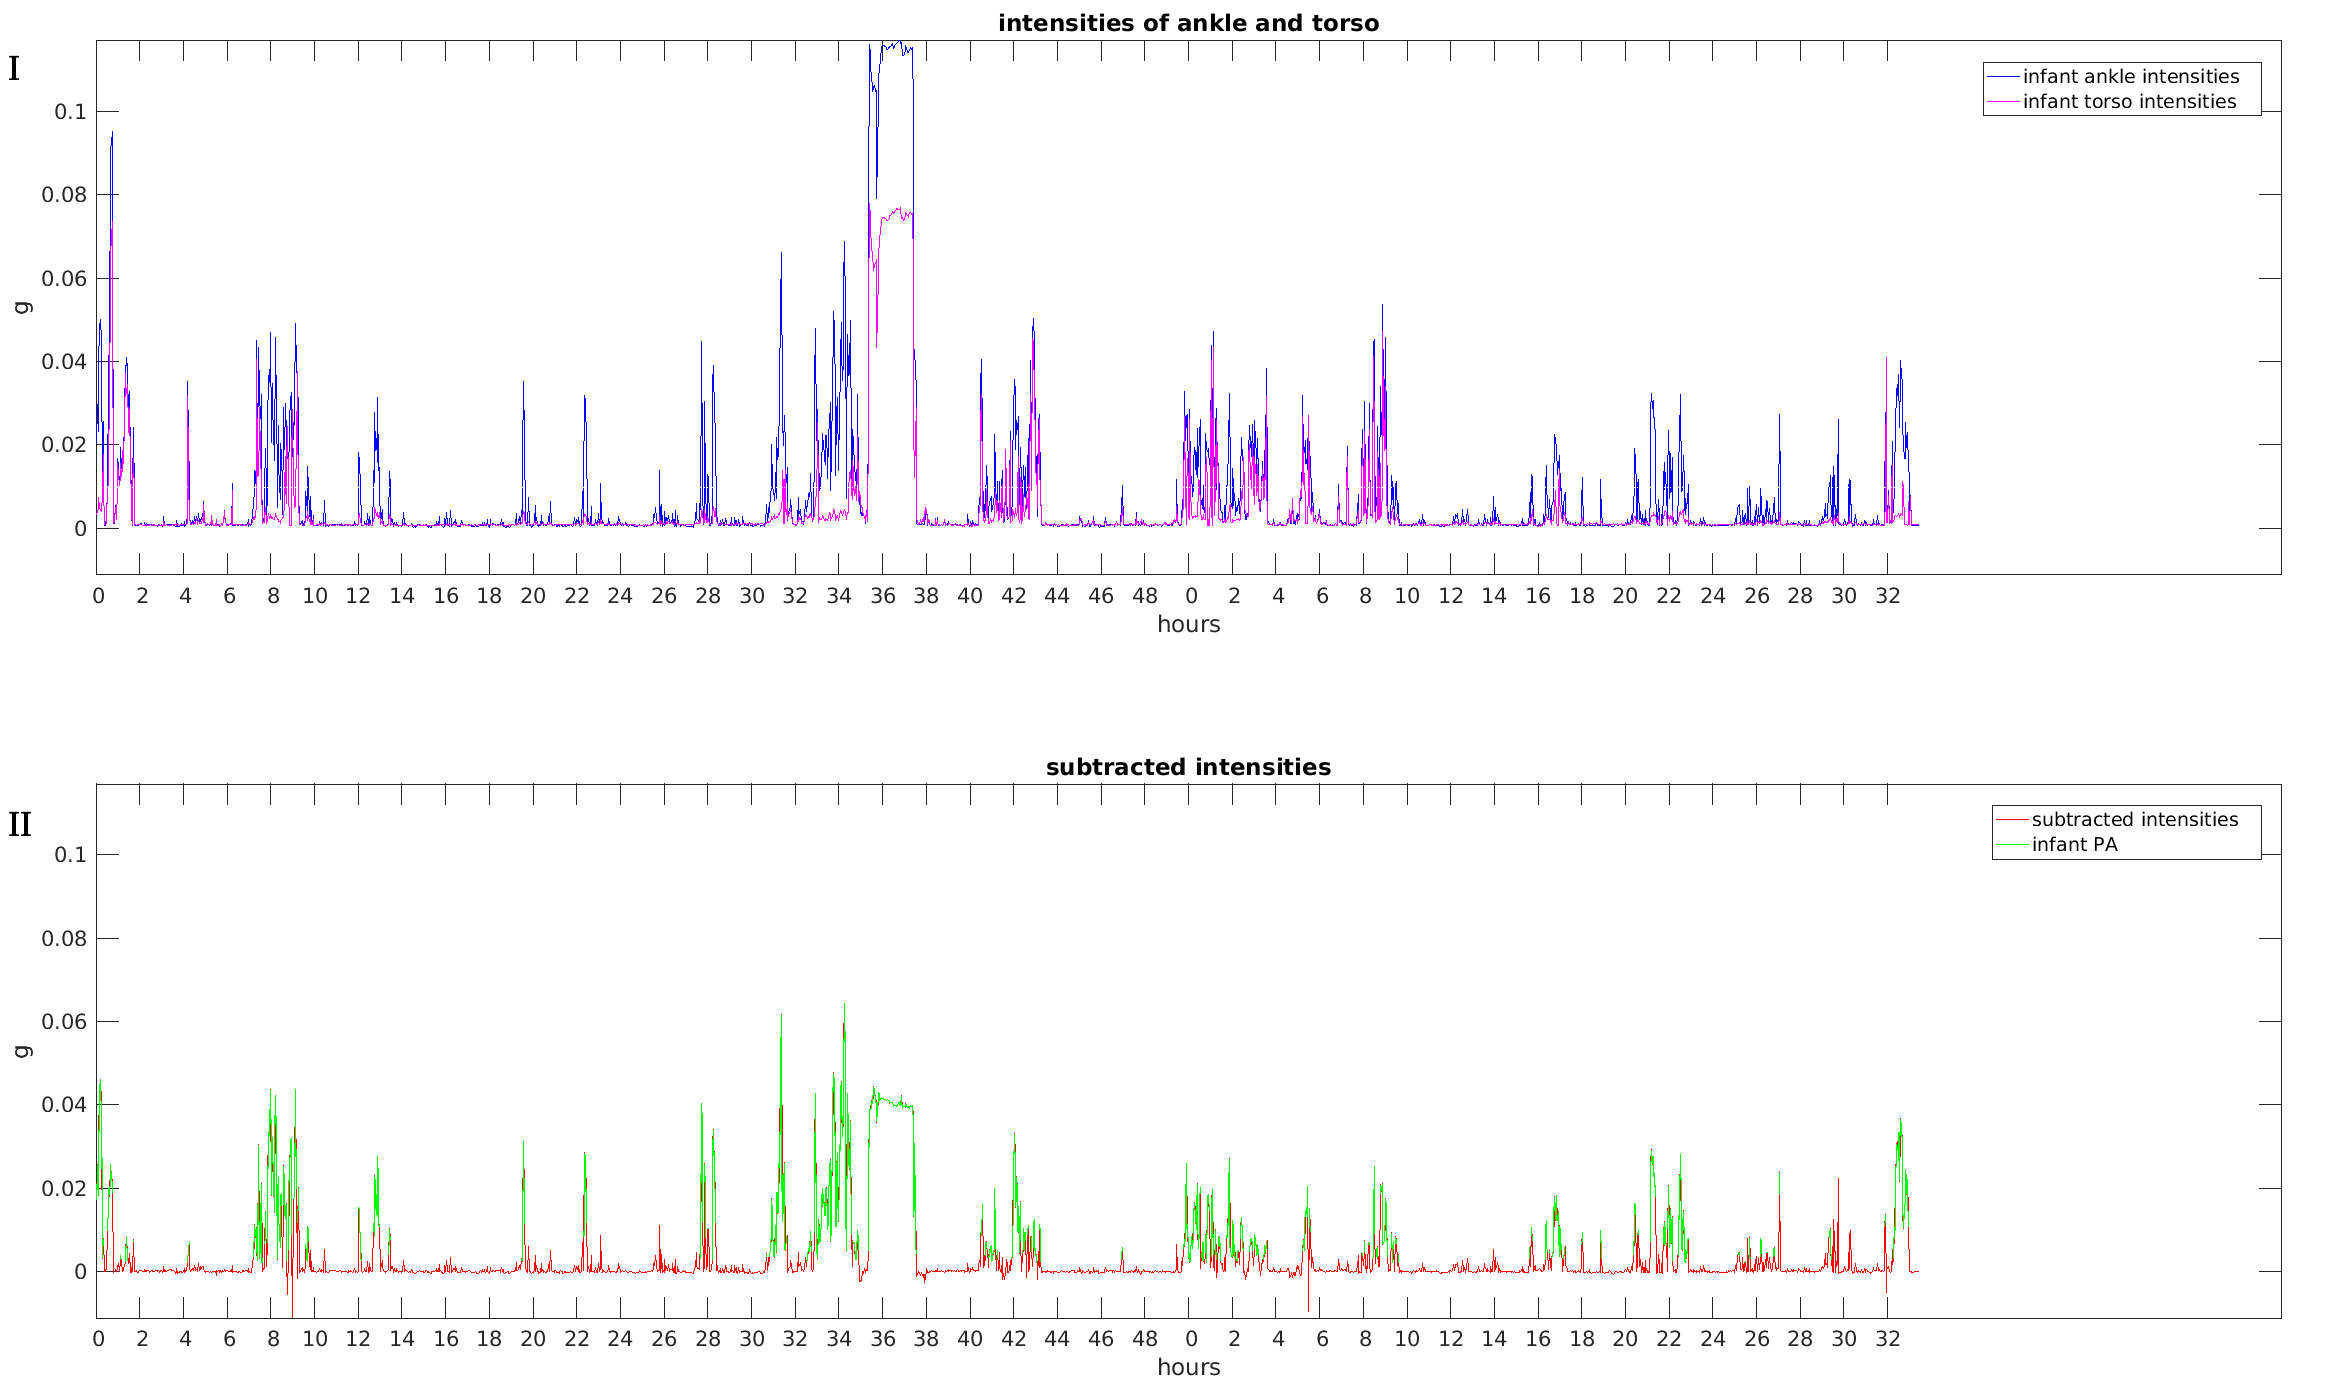
\includegraphics[width=15cm, height=8cm]{SubtractedIntensitiesPA.png}
\caption{PA extraction(II) from the first summary derivation(I), based on approach \textbf{B}.}
\end{figure}

\begin{figure}[h]
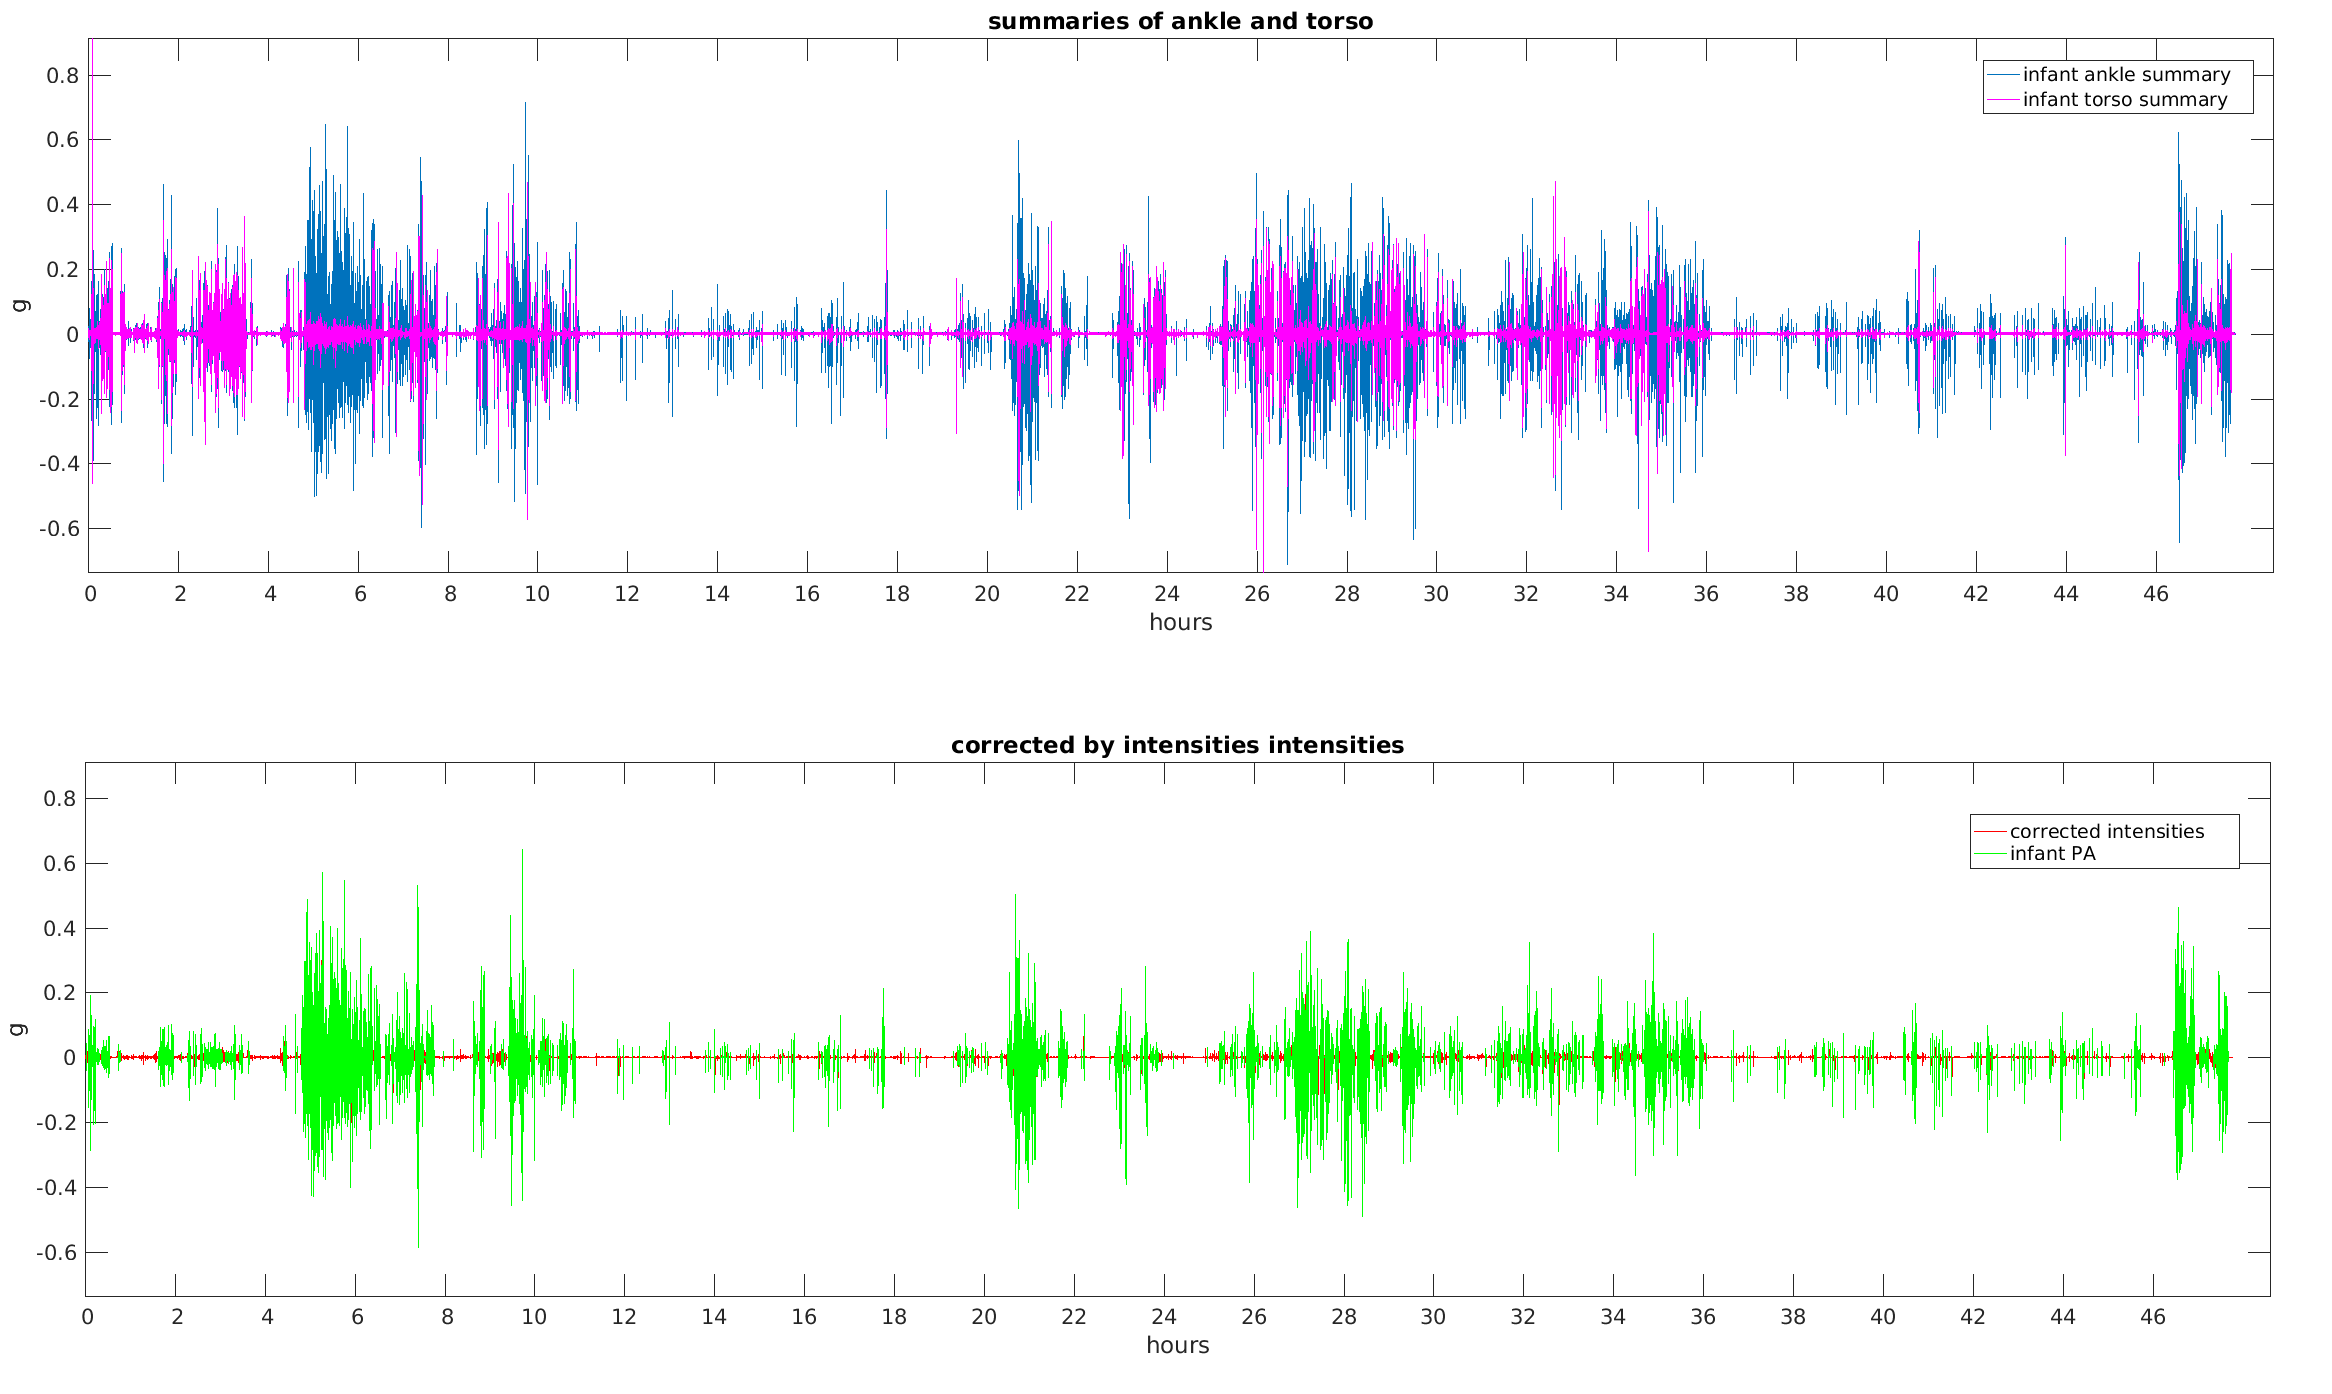
\includegraphics[width=15cm, height=8cm]{CorrectedIntensitiesPA.png}
\caption{PA extraction(II) from the first summary derivation(I), based on approach \textbf{C}.}
\end{figure}
\newpage
\begin{figure}[h!]
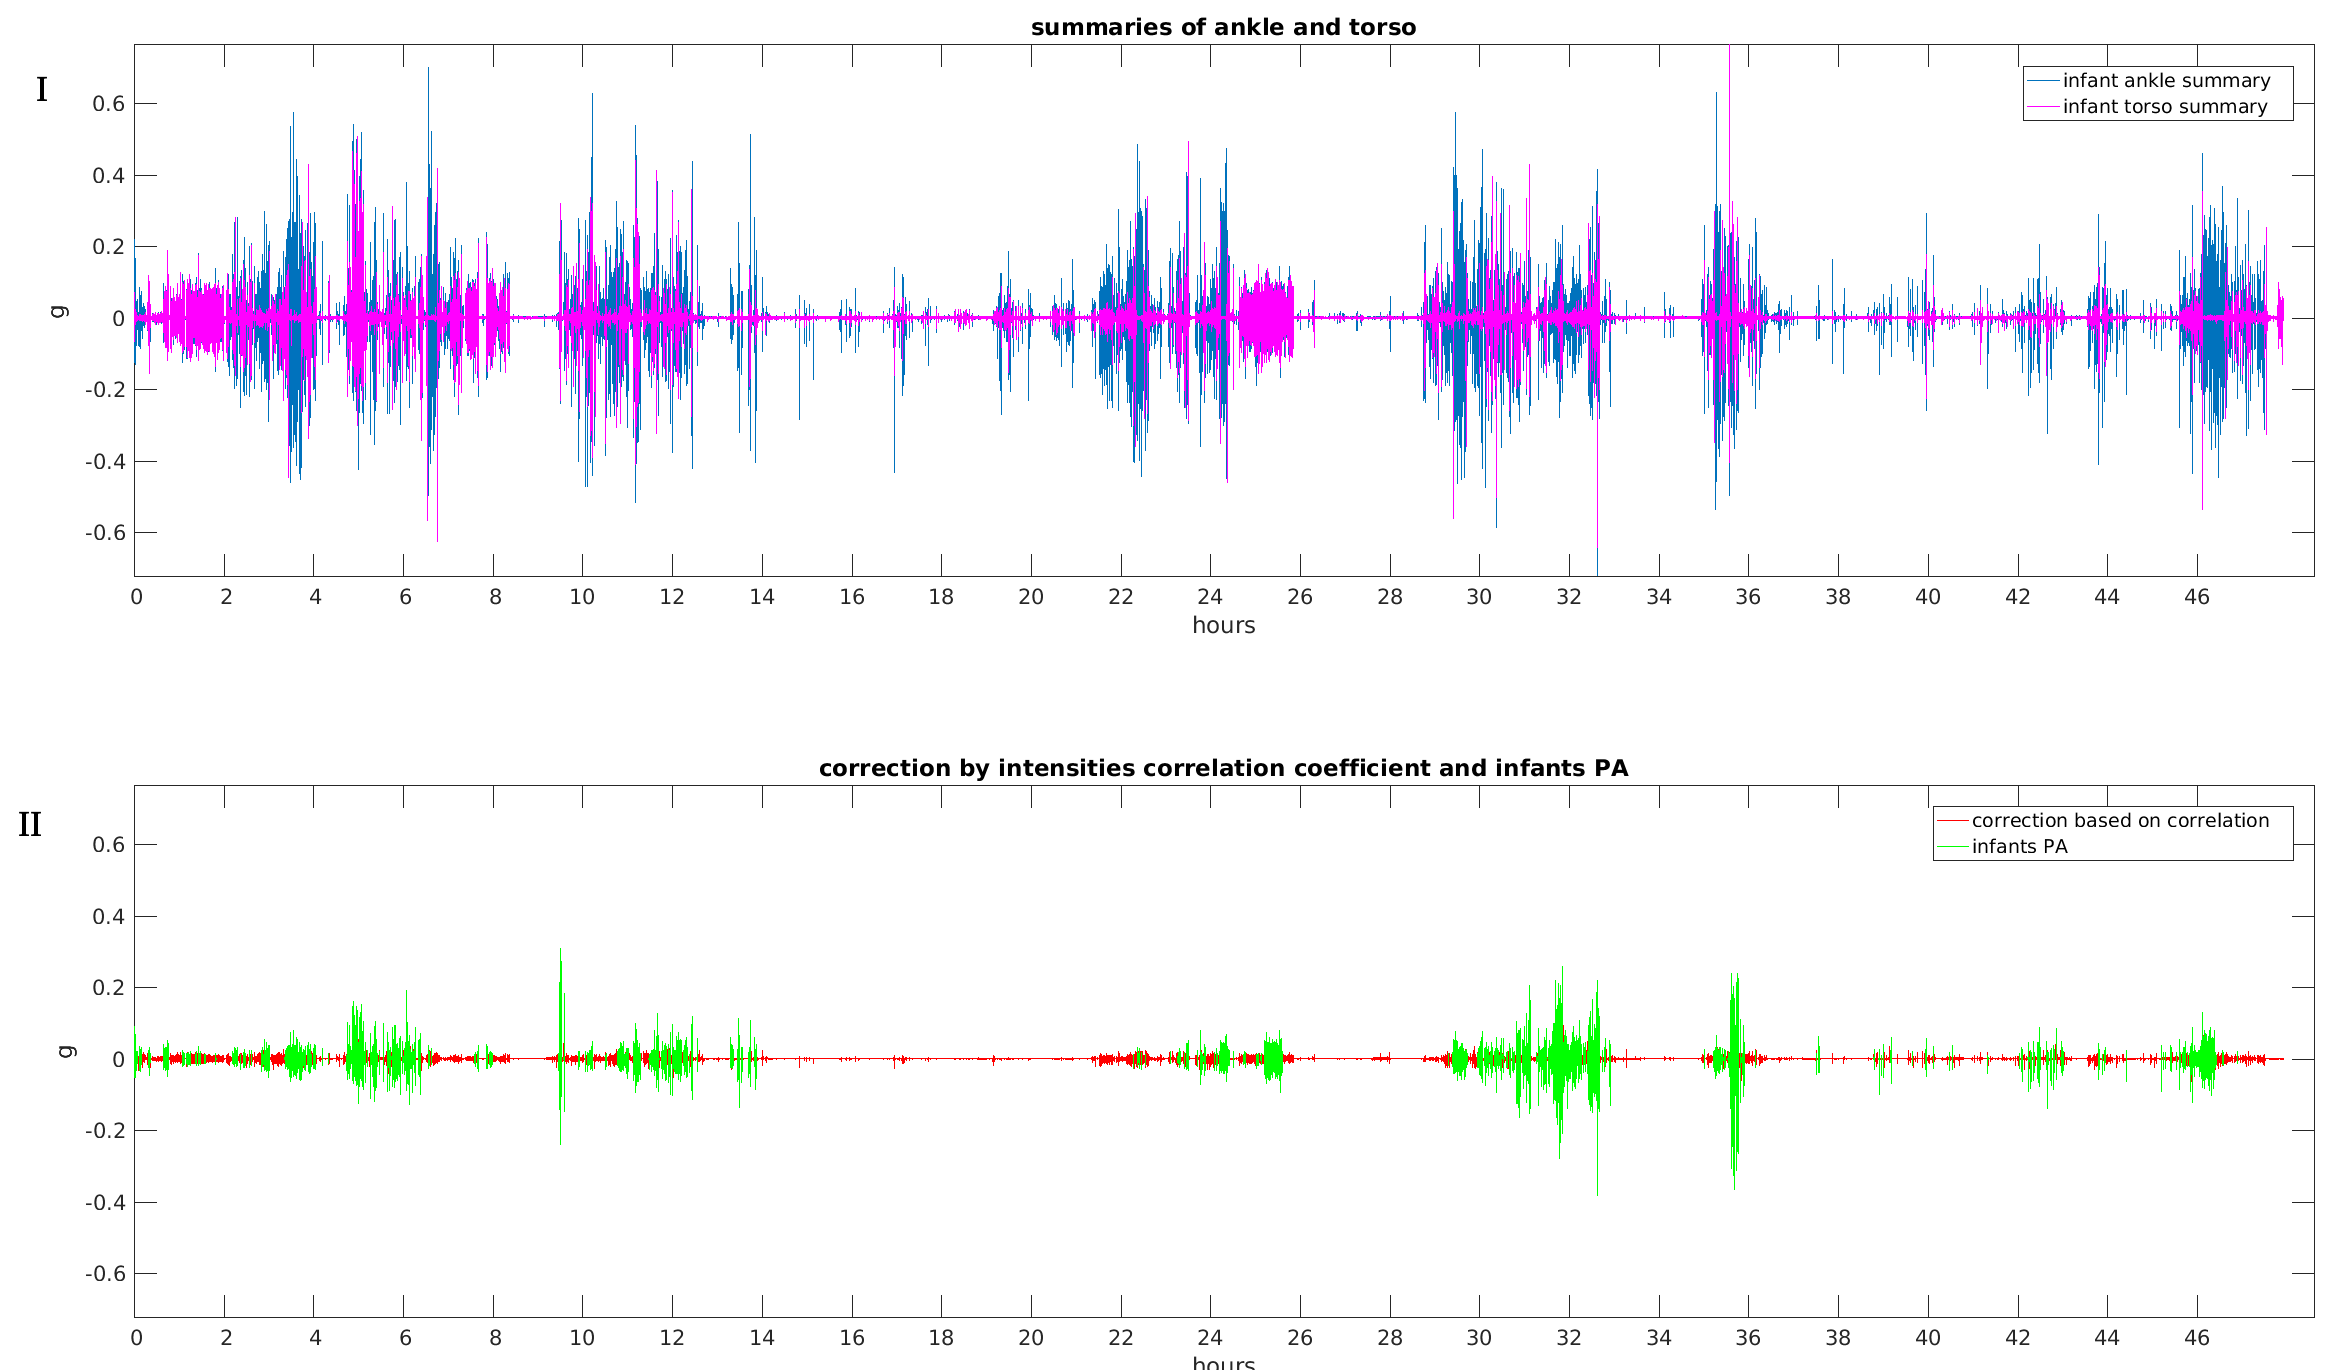
\includegraphics[width=15cm, height=8cm]{CorrectedCorrelationResultPA.png}
\caption{PA extraction(II) from the first summary derivation(I), based on approach \textbf{D}.}
\end{figure}
\\\\
\begin{figure}[h!]
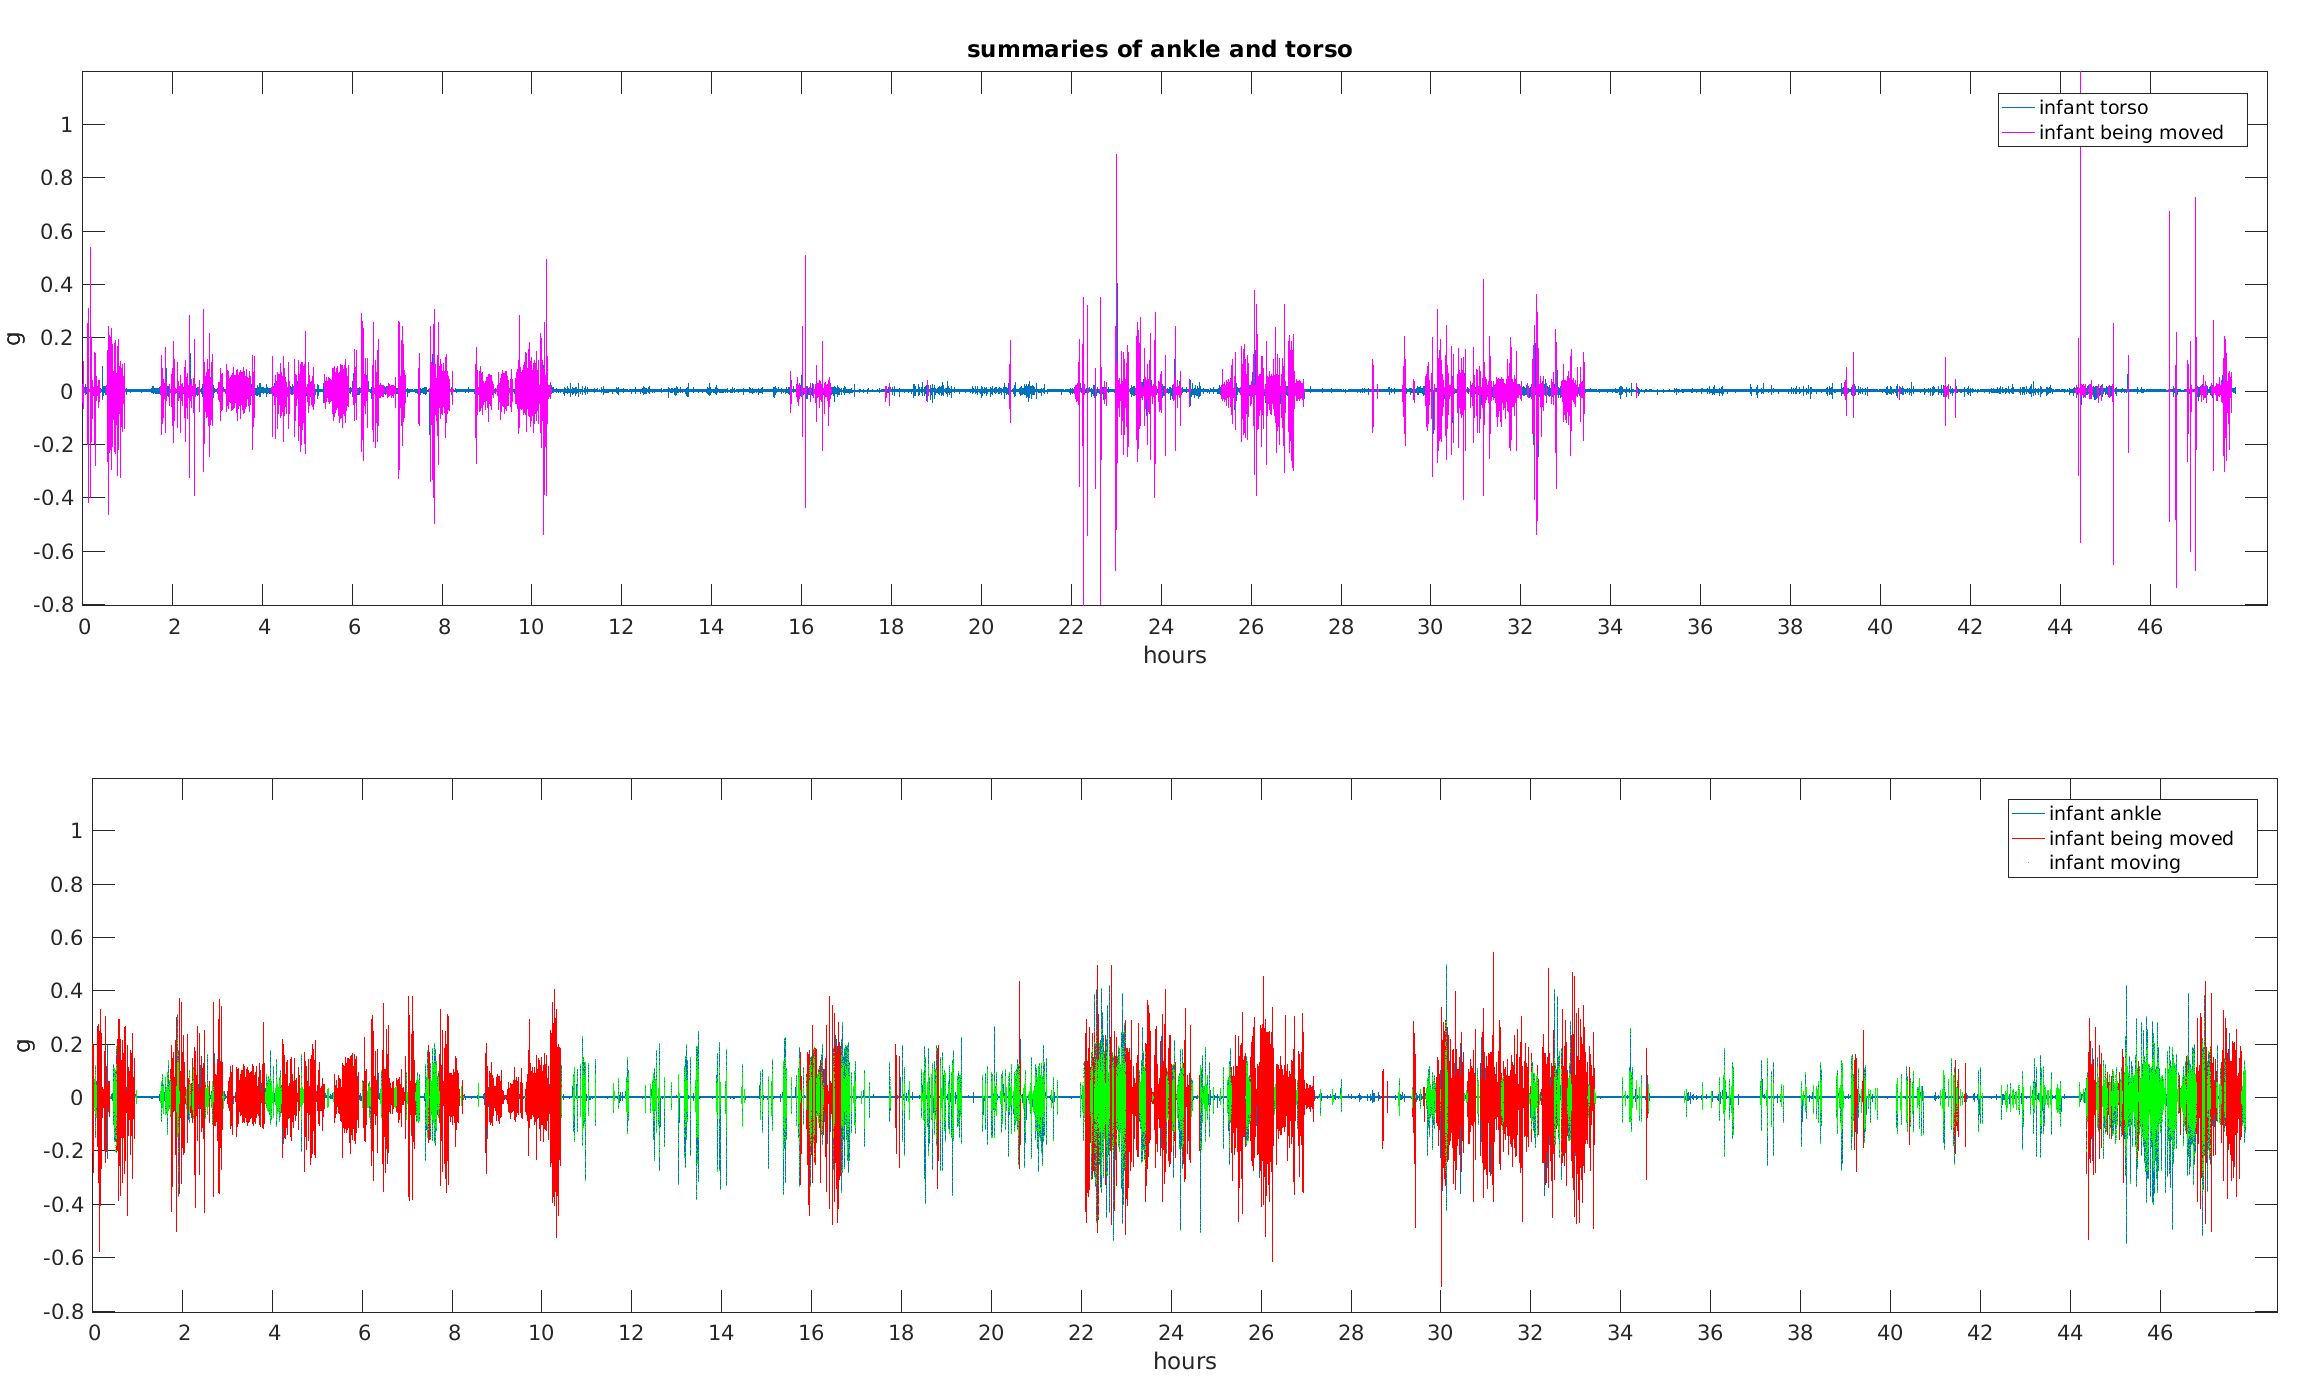
\includegraphics[width=15cm, height=8cm]{approachEPA.png}
\caption{PA extraction(II) from the remaining first summary derivation(I), where all the periods when the infant is detected as being moved (red), are excluded (approach \textbf{E}).}
\end{figure}
\newpage
After each approach, the extraction of PA reflects the consequences of the negative features of the approach. Different outcomes are compared with analysis in the next section.
}
\section{Analysis}
\fontsize{11.25pt}{11.1pt}\selectfont {
The outcomes from different steps of accelerometer data processing are analyzed, compared and assessed, in order to obtain the most appropriate extraction of infants PA levels, focusing on validity and feasibility of extraction. Non-wear time detection is a relatively simple and straight forward procedure, therefore the outcome is examined briefly, while outcomes of summary derivation and correction of caretakers contributions are examined more considerately. The two different types of summary derivations are compared, and their within subject variance examined along with the proportion of smaller accelerations on the torso placed measurement. Outcomes of different approaches for correction of caretakers contributing accelerations are compared for both types of summary derivation, based on the increase or decrease of the windowed SD and absolute intensities. Further more, in the approach \textbf{E}, the total final proportion of time the infant is detected as being moved is compared between the two types of summary derivation and for different thresholds for SD. For the most appropriate threshold, the values of the absolute correlation coefficients, presenting similarity between torso and ankle, are analyzed between the time the infant is detected as being moved and the remaining time. In further analysis, the proportion of time where PA was detected is analyzed along with the proportions of time the infant is detected as being moved.\\
In the end, the results from the analysis are compared against the diary notations of infants sleeping and feeding habits, to assess the validity and feasibility of infants PA measure, while considering the reliability and plausibility of the validation method itself.

\subsection{Results}
\\
All together 12 out of 30 infants had non-wear time detected on the torso accelerometer, with an average of 8.6\% of data being removed with minimum 1.2\% and maximum 31.1\%. One of the infants had also had the ankle accelerometer removed at the end of the 48 hour time period. The data points from the non-wear time detected in infant ankle and torso placed accelerometer are removed from all measurements, while the data points from the non-wear time detected in the maternal accelerometer data are only removed from the maternal accelerometer data. The start and end timestamps of all blocks of data points detected as non-wear, are saved to enable validation against the diaries.\\
When analyzing the difference between the two types of summary derivation and the amount of variance interfered, two windowed descriptive statistics are examined, SD and absolute intensity. Windowed descriptive statistics are calculated for each of the 30 subjects, corresponding torso and ankle placed measurements and corresponding two types of summary derivation. Additionally, windowed proportions of smaller accelerations on the torso placed measurement are extracted and compared between the two types of summary derivation. For all descriptive statistics, mean and variance is compared between the two types of summary derivation. For the majority, the comparisons are done with a Wilcoxon signed-rank test, while the normally distributed means and variances of the proportions of smaller accelerations on the torso placed measurement are compared with a t.test. All comparisons showed significant differences in the means and variances of the descriptive statistics between the two differently placed monitors, with all p-values below 0.0001. In figure 22 and 23, violin plots show the differences in the windowed SD and absolute intensities between the two types of summary derivation, respectively. Even though the degree of difference varies between the differently placed monitors and amongst subjects, it is apparent the SD and absolute intensities are higher in the second type of summary derivation with a different distribution. Consequently, the results from further processing and analysis, of the two types of summary derivation, have to be compared with caution. Boxplots for the simple proportions of smaller accelerations on the torso are shown in Figure 24.

\begin{figure}[h]
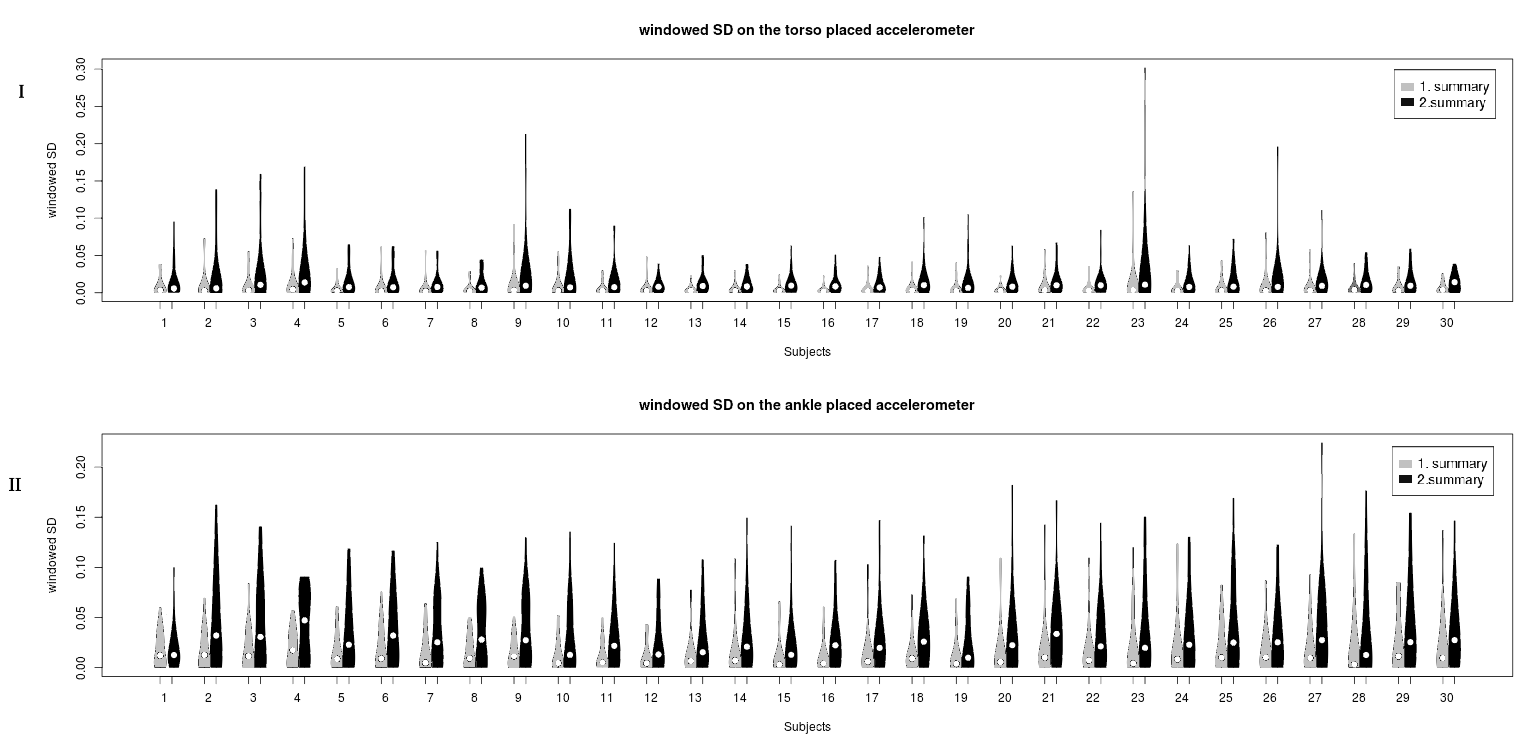
\includegraphics[width=15cm, height=8cm]{final_violplot_SD.png}
\caption{Violin plot showing the differences between the windowed SD of the two types of summary derivation for the torso(I) and ankle(II) placed measurements.}
\end{figure}
\newpage
\begin{figure}[h!]
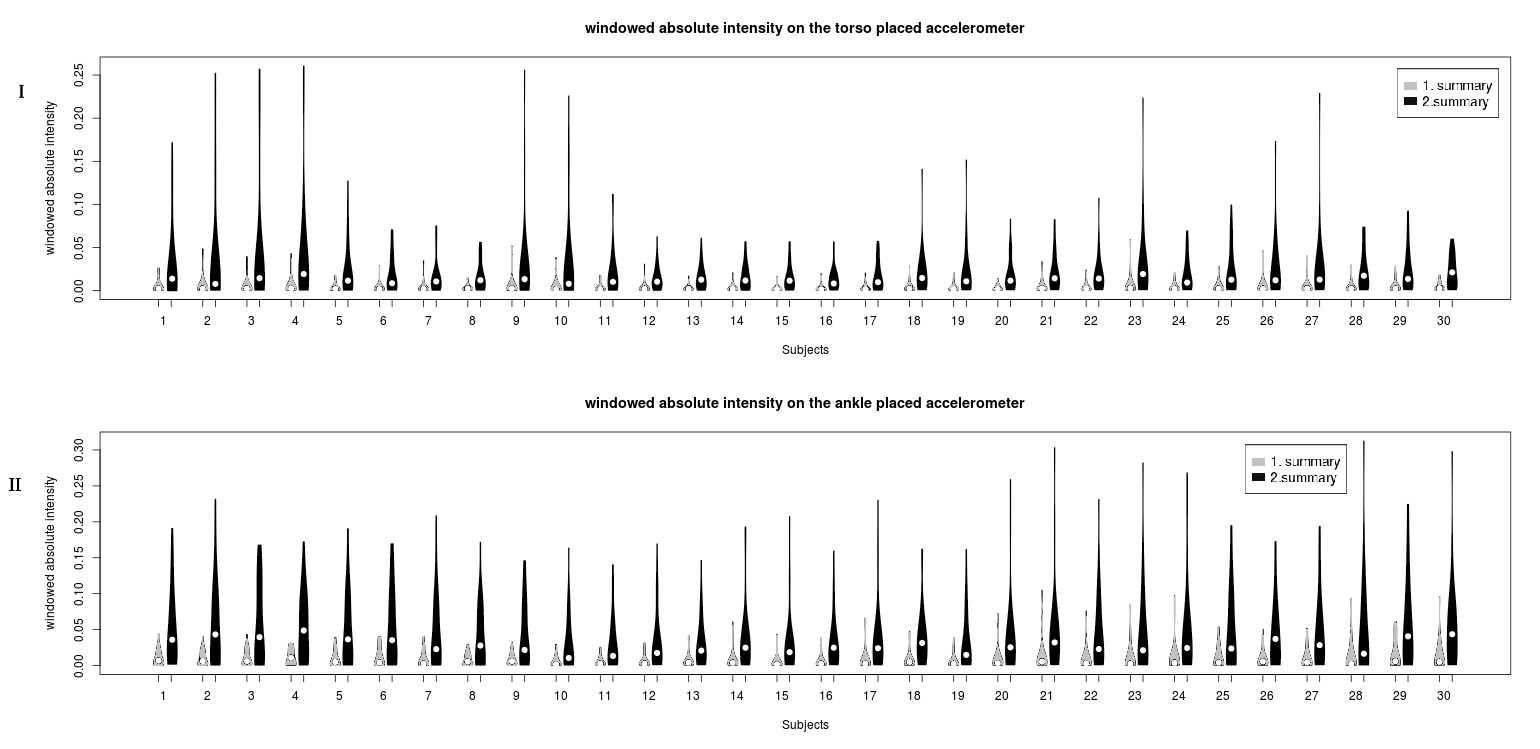
\includegraphics[width=15cm, height=8cm]{final_violplot_AI.png}
\caption{Violin plot showing the differences between the windowed absolute intensity of the two types of summary derivation for the torso(I) and ankle(II) placed measurements.}
\end{figure}

\begin{figure}[h!]
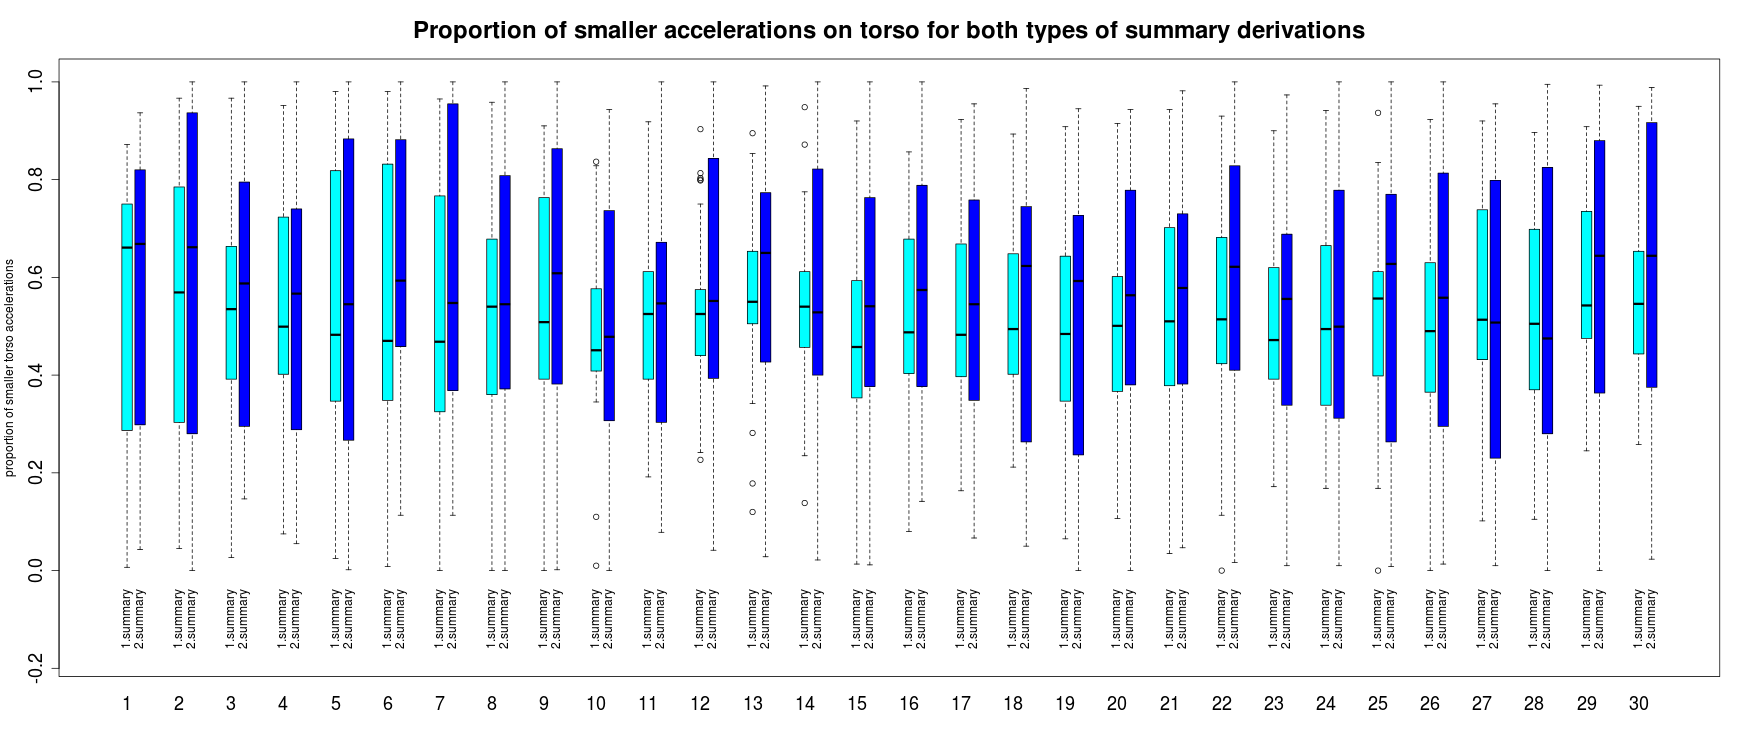
\includegraphics[width=15cm, height=8cm]{final_proportions_boxplot.png}
\caption{Box plot showing the differences and variation in differences between the two types of summary derivation for a simple measure of the proportion of smaller accelerations on the torso placed measurement.}
\end{figure}
\newpage
Plots and statistical analyses showed that the two types of summary derivation produce a different scale for the acceleration size and that second summary derivation has a higher within subject variation. While this is a good example why caution is required when summarizing accelerometer data and choosing appropriate thresholds, the source of variation is unknown and causing uncertainty regarding the best choice of summary derivation. For this reason, two types of summary derivation are analyzed further, by comparing and analyzing the outcomes of different approaches correcting the caretakers contributing accelerations. In Figures 25-30, boxplots show the overall increase or decrease of the descriptive statistics after the different approaches. Table 1, shows the overall increase or decrease of descriptive statistics in percentage.
\\
\begin{figure}[h!]
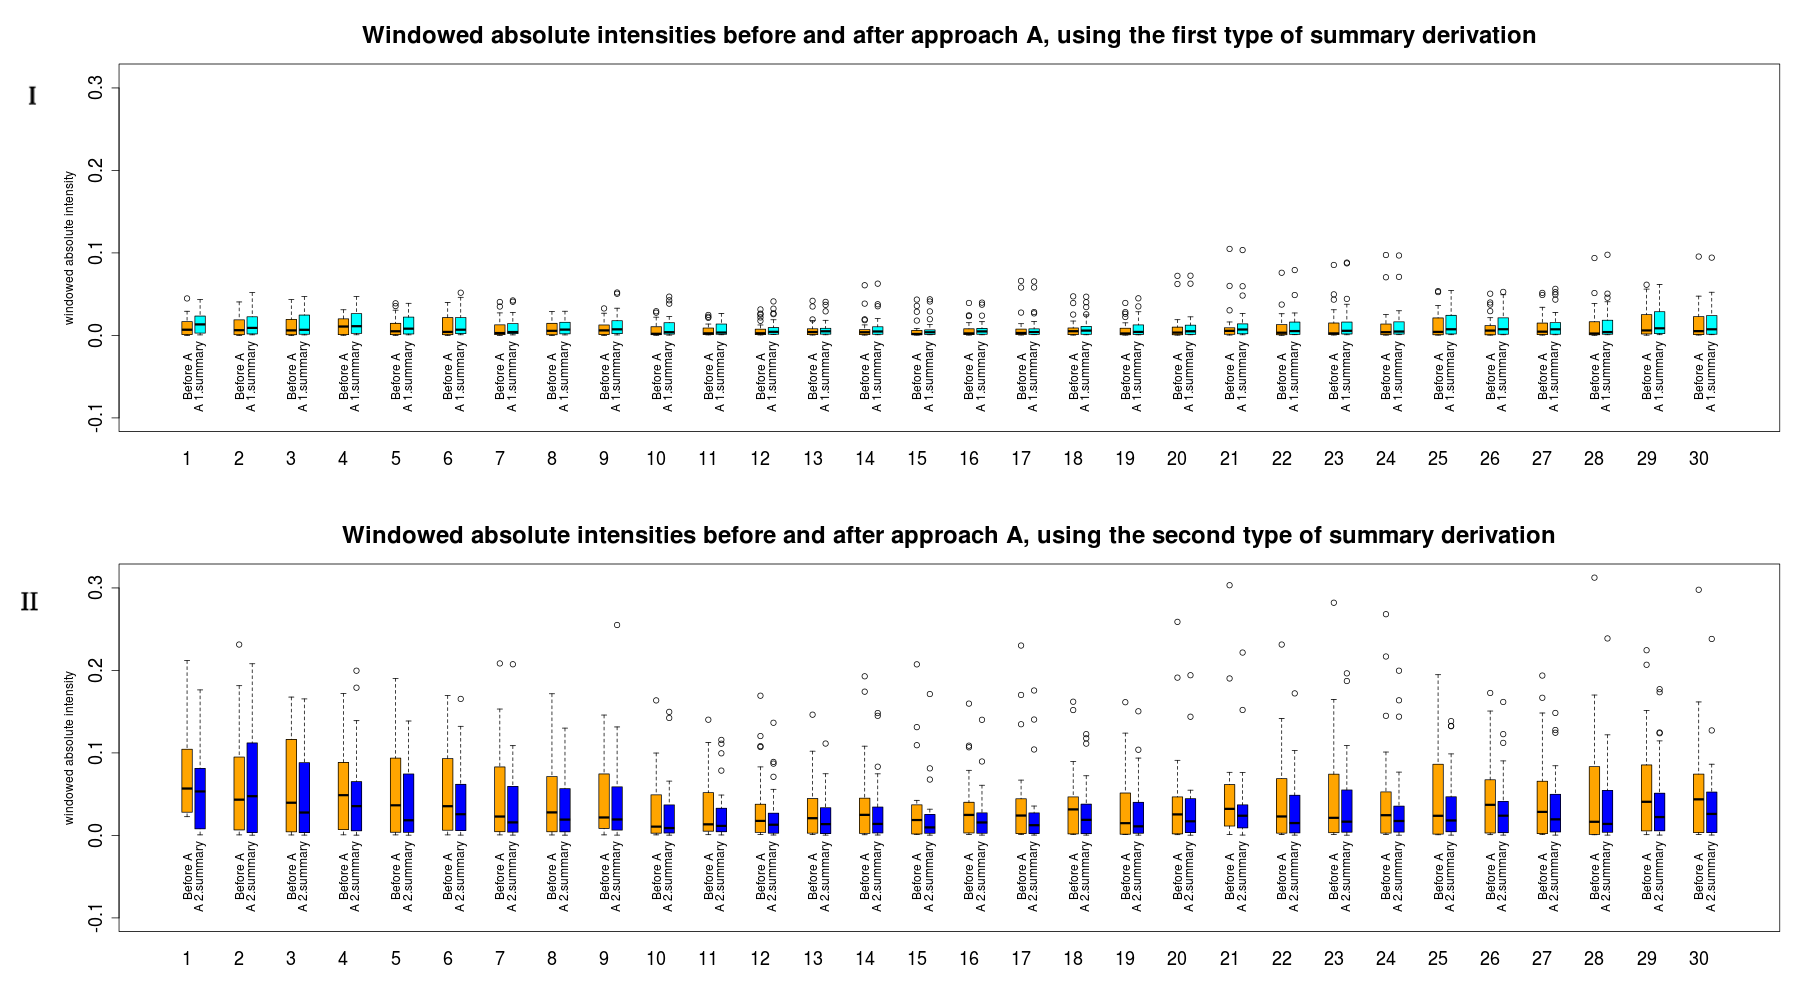
\includegraphics[width=15cm, height=8.5cm]{result_approach_A_AI_boxplot.png}
\caption{Boxplots showing windowed absolute intensities, before(I) and after(II) correcting the contributing acceleration with the approach A, based on the two different types of summary derivation.}
\end{figure}
\newpage
\begin{figure}[h!]
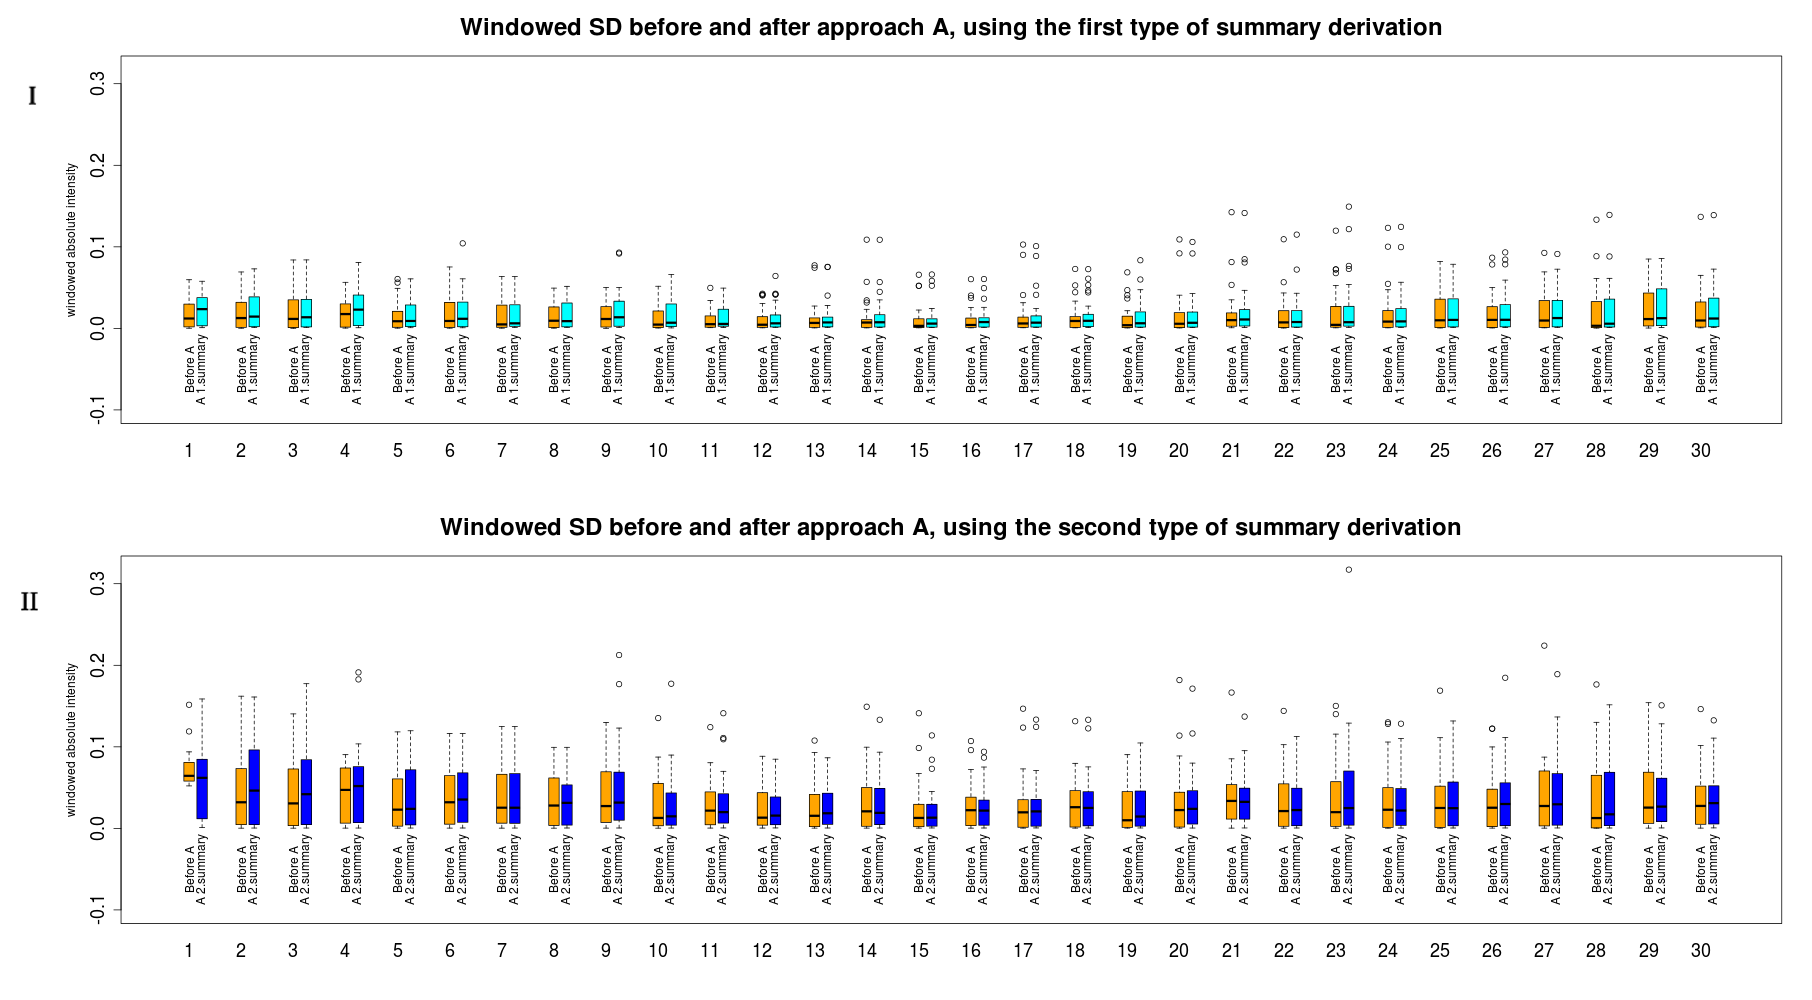
\includegraphics[width=15cm, height=8.5cm]{result_approach_A_SD_boxplot.png}
\caption{Boxplots showing windowed SD, before(I) and after(II) correcting the contributing acceleration with the approach A, based on the two different types of summary derivation.}
\end{figure}

\begin{figure}[h!]
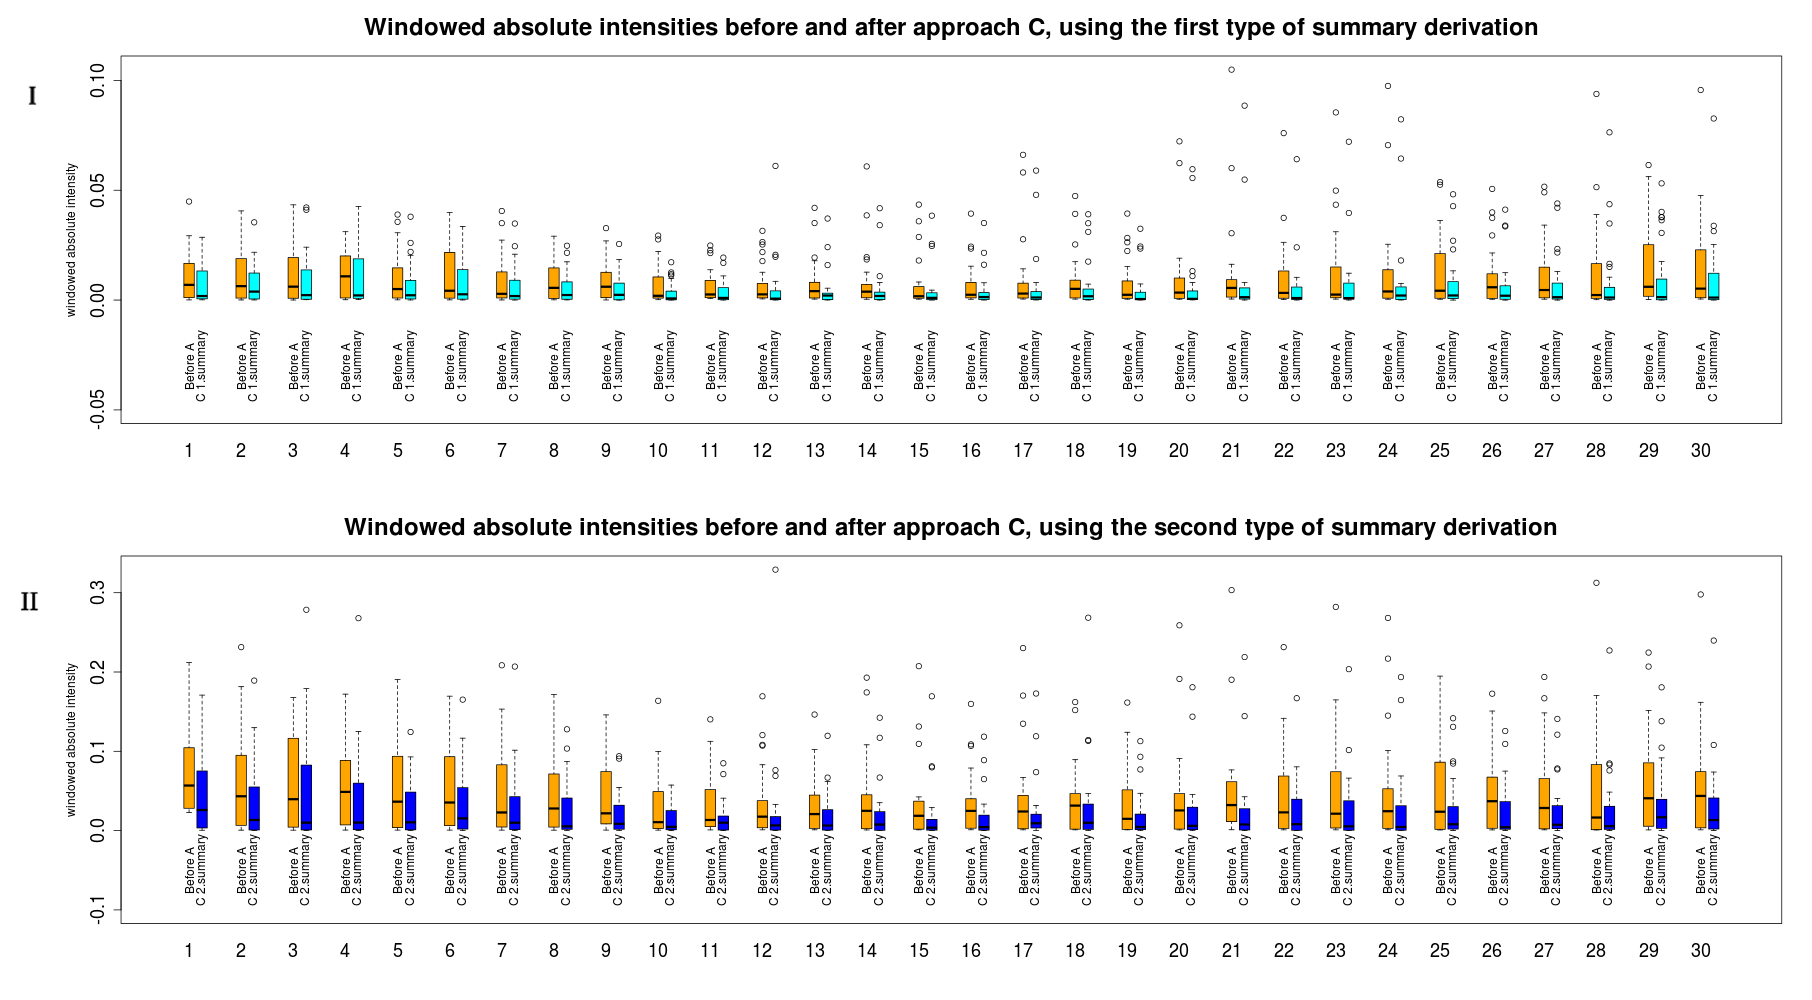
\includegraphics[width=15cm, height=8.5cm]{result_approach_C_AI_boxplot.png}
\caption{Boxplots showing windowed absolute intensities, before(I) and after(II) correcting the contributing acceleration with the approach C, based on the two different types of summary derivation.}
\end{figure}
\newpage
\begin{figure}[h!]
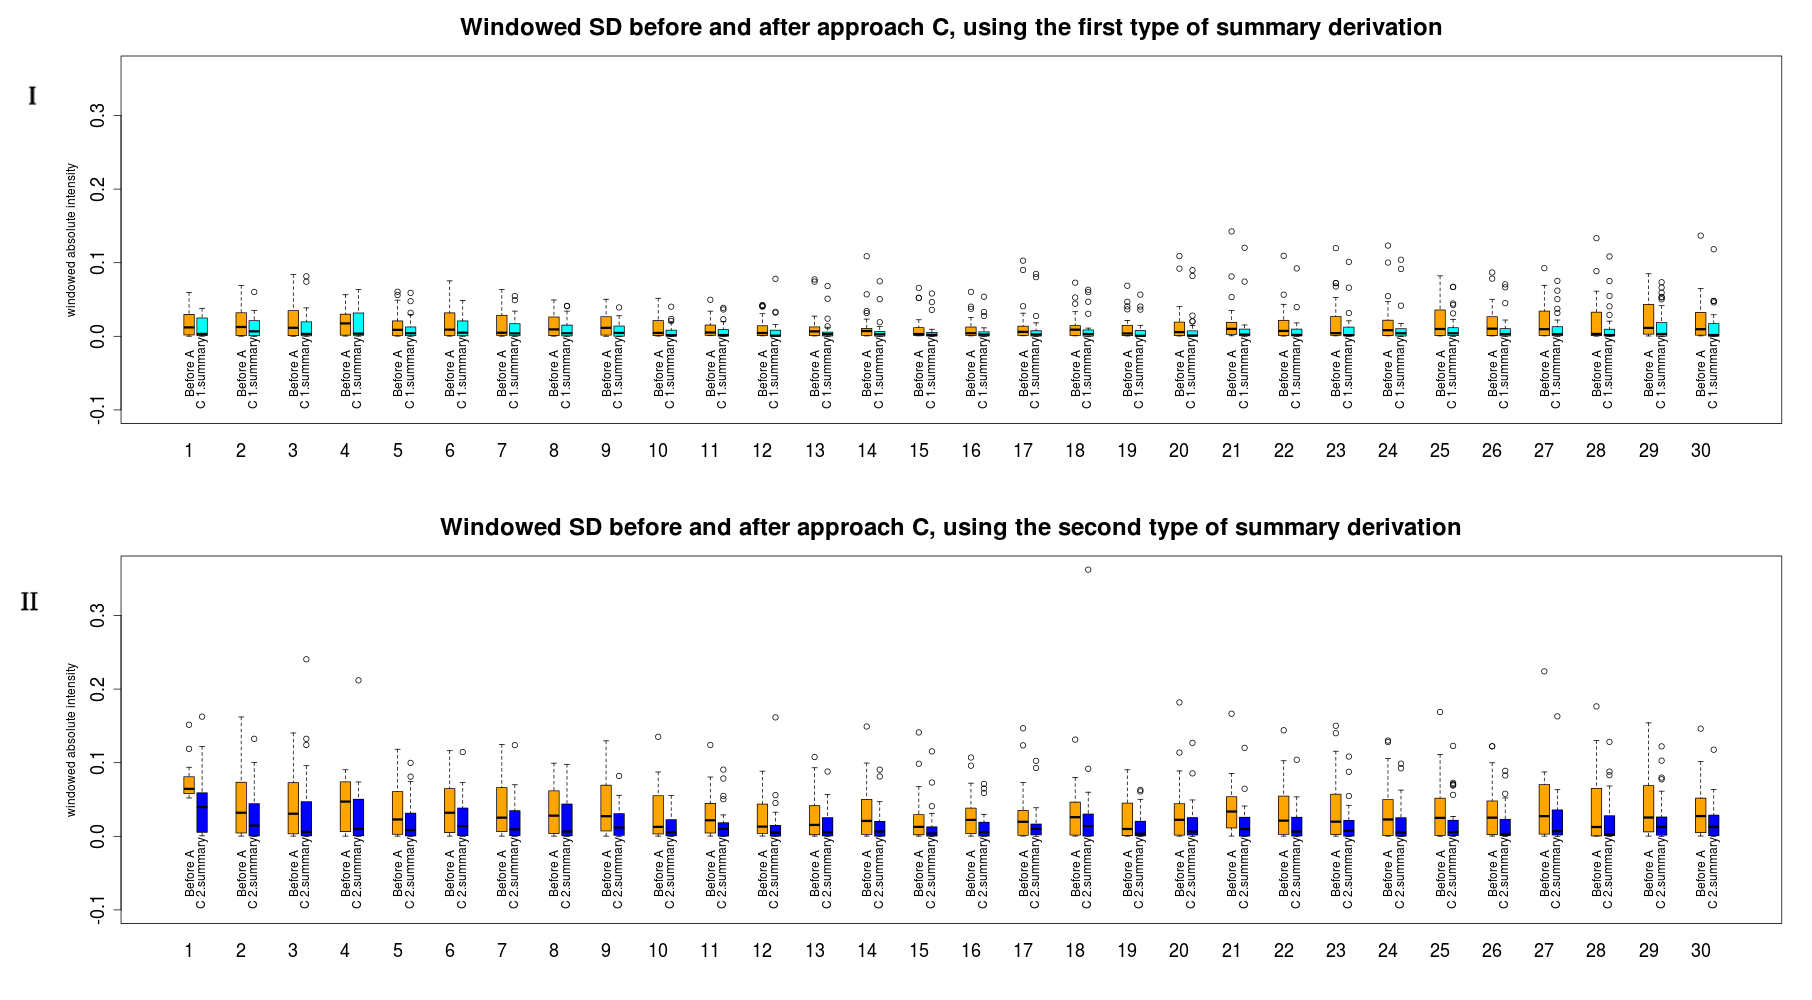
\includegraphics[width=15cm, height=8.5cm]{result_approach_C_SD_boxplot.png}
\caption{Boxplots showing windowed SD, before(I) and after(II) correcting the contributing acceleration with the approach C, based on the two different types of summary derivation.}
\end{figure}

\begin{figure}[h!]
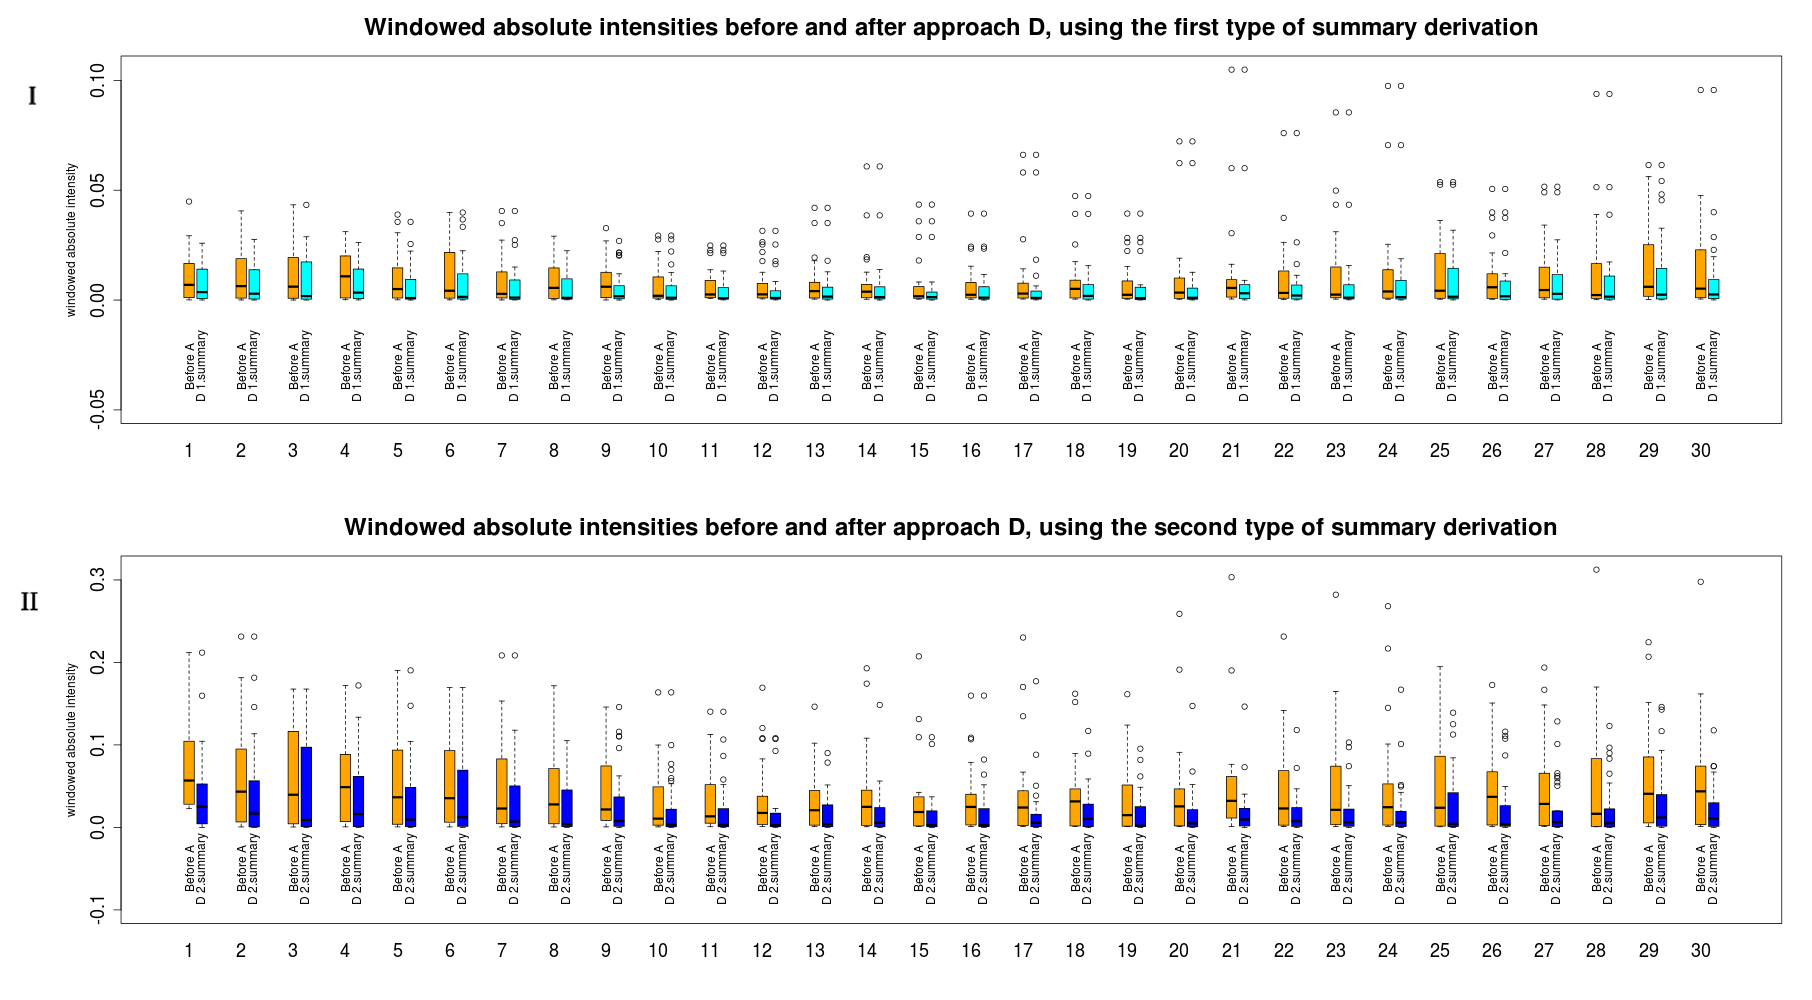
\includegraphics[width=15cm, height=8.5cm]{result_approach_D_AI_boxplot.png}
\caption{Boxplots showing windowed absolute intensities, before(I) and after(II) correcting the contributing acceleration with the approach D, based on the two different types of summary derivation.}
\end{figure}
\newpage
\begin{figure}[h!]
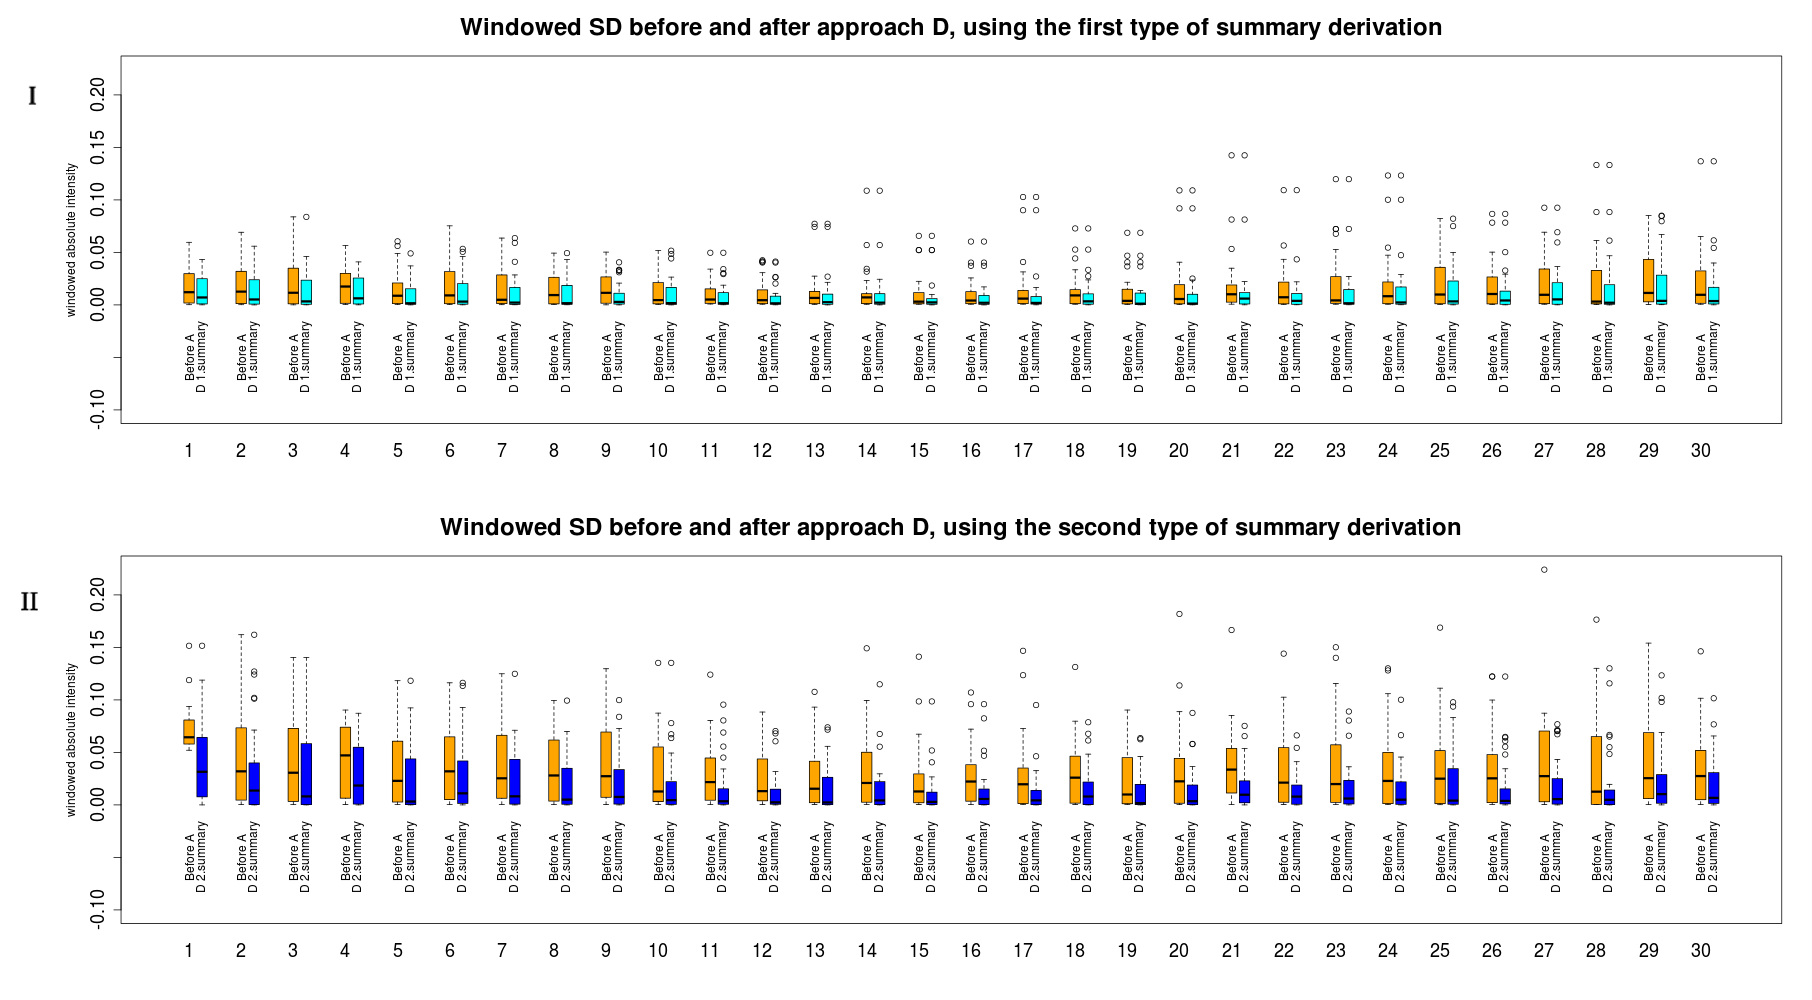
\includegraphics[width=15cm, height=8.5cm]{result_approach_D_SD_boxplot.png}
\caption{Boxplots showing windowed SD, before and after correcting the contributing acceleration with the approach D, based on the two different types of summary derivation.}
\end{figure}

% Please add the following required packages to your document preamble:
% \usepackage{multirow}
\begin{table}[h!]
\centering
\begin{tabular}{|c|c|c|c|c|c|c|}
\hline
\multirow{2}{}{} & \multicolumn{2}{c|}{\textbf{approach A}} & \multicolumn{2}{c|}{\textbf{approach C}} & \multicolumn{2}{c|}{\textbf{approach D}} \\ \cline{2-7} 
 & SD & \begin{tabular}[c]{@{}l@{}}absolute\\ intensity\end{tabular} & SD & \begin{tabular}[c]{@{}l@{}}absolute\\ intensity\end{tabular} & SD & \begin{tabular}[c]{@{}l@{}}absolute\\ intensity\end{tabular} \\ \hline
\textbf{\begin{tabular}[c]{@{}l@{}}first type of\\ summary derivation\end{tabular}} & 21.38\% & 28.08\% & -43.95\% & -44.98\% & -56.82\% & -57.07\% \\ \hline
\textbf{\begin{tabular}[c]{@{}l@{}}second type\\ of summary derivation\end{tabular}} & 7.80\% & -23.61\% & -42.40\% & -43.36\% & -63.20\% & -63.46\% \\ \hline
\end{tabular}
\caption{Mean change of the descriptive statistics in proportions after the different approaches.}
\end{table}
\newpage
Although the boxplots appear different for the two types of summary derivation, the results are more similar, with the exception of the approach A. Overall, the second type of summary derivation has slightly better results, which is to be confirmed with further analysis.
\\Approach \textbf{E} has not yet been included in the analysis, since the principal is different. In approach \textbf{E}, the periods when the infant is being moved are not attempted to be corrected, but are simply removed. If one would like to strictly analyze infants activity patterns only, approach \textbf{E} should be the most appropriate, since the caretaker will not only confound the amount of accelerations, but also the overall movement of the infant, for example by stimulation, restriction by holding, reduction due to diversion of attention etc.
Ideally, the approach for correcting caretakers contributing accelerations should only remove periods when the infant is being moved. Accurate detection of these periods exceeds the work of this project.\\Cut-point for SD was set empirically and tested for best results. Since the outcomes of the two different types of summary derivation are significantly different, different cut-points had to be set for each summary, while seeking the highest correlation between the percentages of final time detected as being moved for all subjects. Spearmans rank correlation coefficient was the highest at 0.8603, with a p-value below 0.00001, for a cut-point 0.006g for the first type of summary derivation and 0.0185g for the second type. Figure 31 shows the scatter plot of the percentages of being moved time for all 30 subjects of the first type of summary derivation versus the second type, with the highest correlation coefficient.
\begin{figure}[h!]
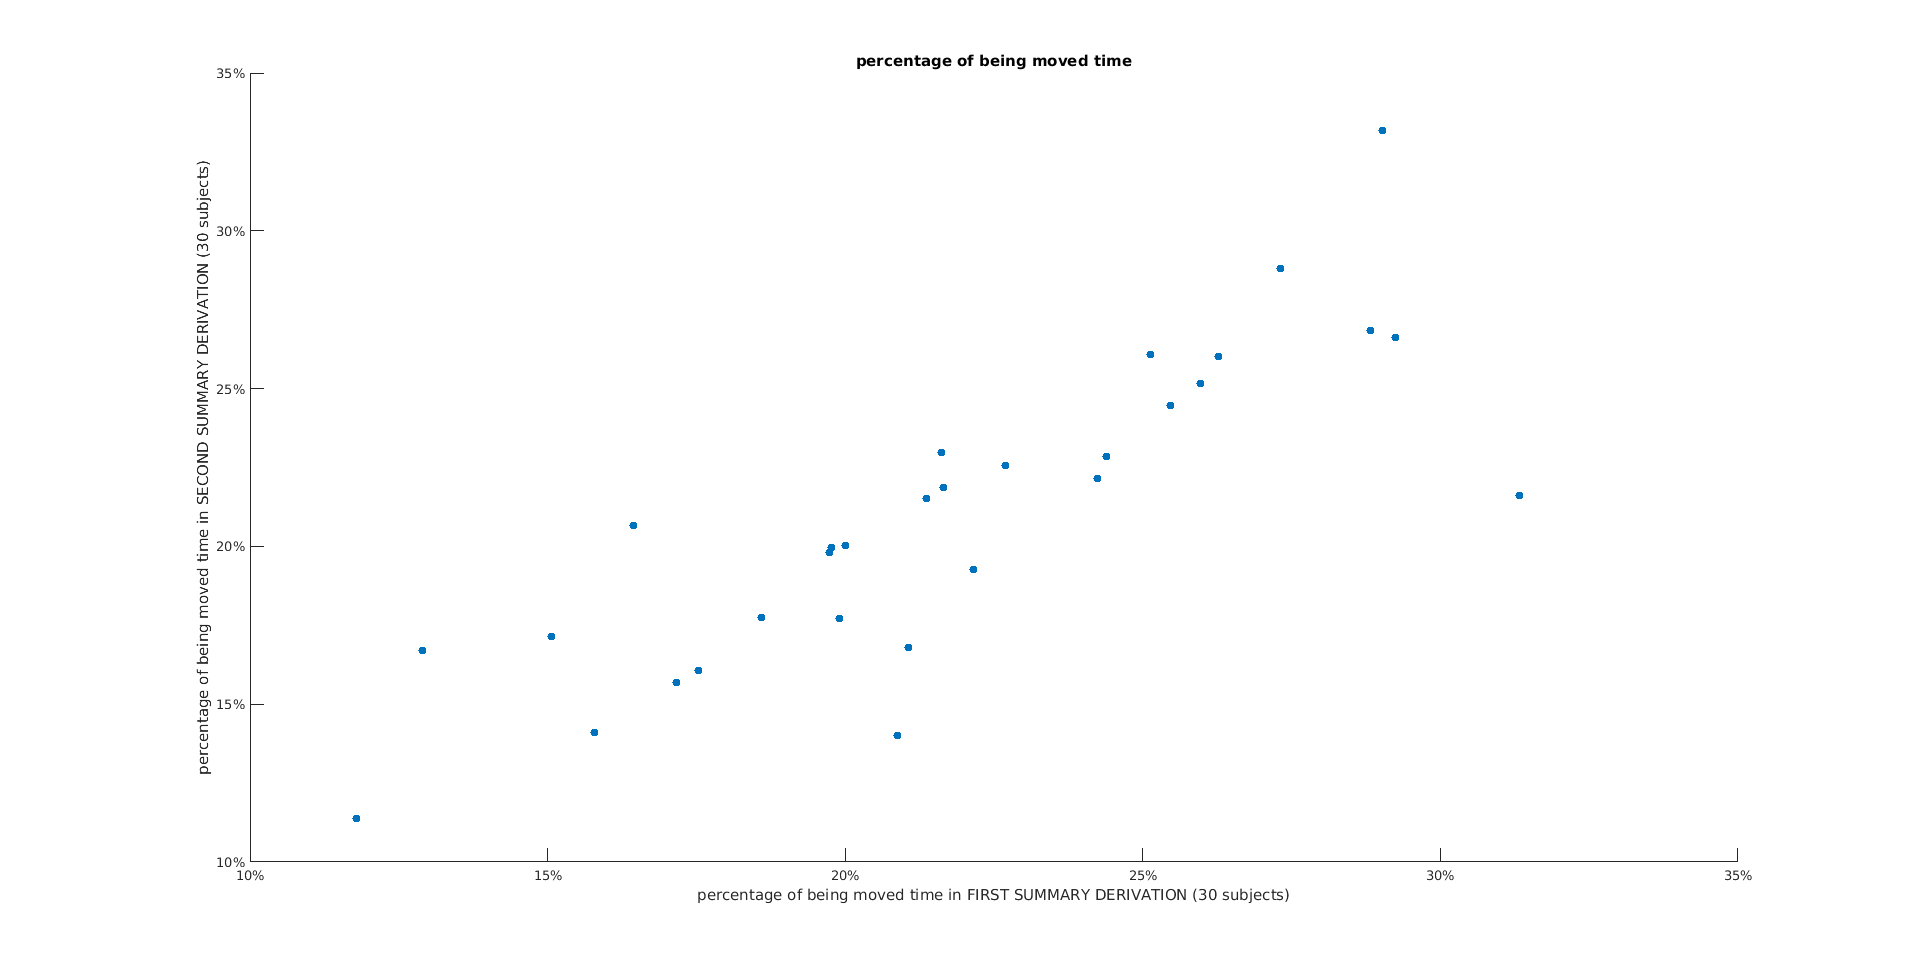
\includegraphics[width=15cm, height=8.5cm]{approach_E_correlation_being_moved.png}
\caption{Scatter plot showing the percentages of being moved time, which were most correlated for all 30 subjects, for the first summary derivation on the x axis and the second type on the y axis.}
\end{figure}

\newpage
Having the approximate periods where the infant was being moved, the absolute correlation coefficient between the accelerations on the torso placed measurement and the ankle placed measurement can be analyzed, in order to further assess the two types of summary derivation. Figures 32 and 33 show the absolute windowed Pearsons correlation coefficient for the accelerations of the torso and ankle placed measurements, grouped according to whether the infant was detected as being moved or not, for the first and second type of summary derivation respectively. Figure 34 shows the absolute correlation coefficient distribution for the two types of summary derivation and the corresponding periods where the infant was detected as being moved and where it was not.
\newpage
\begin{figure}[h!]
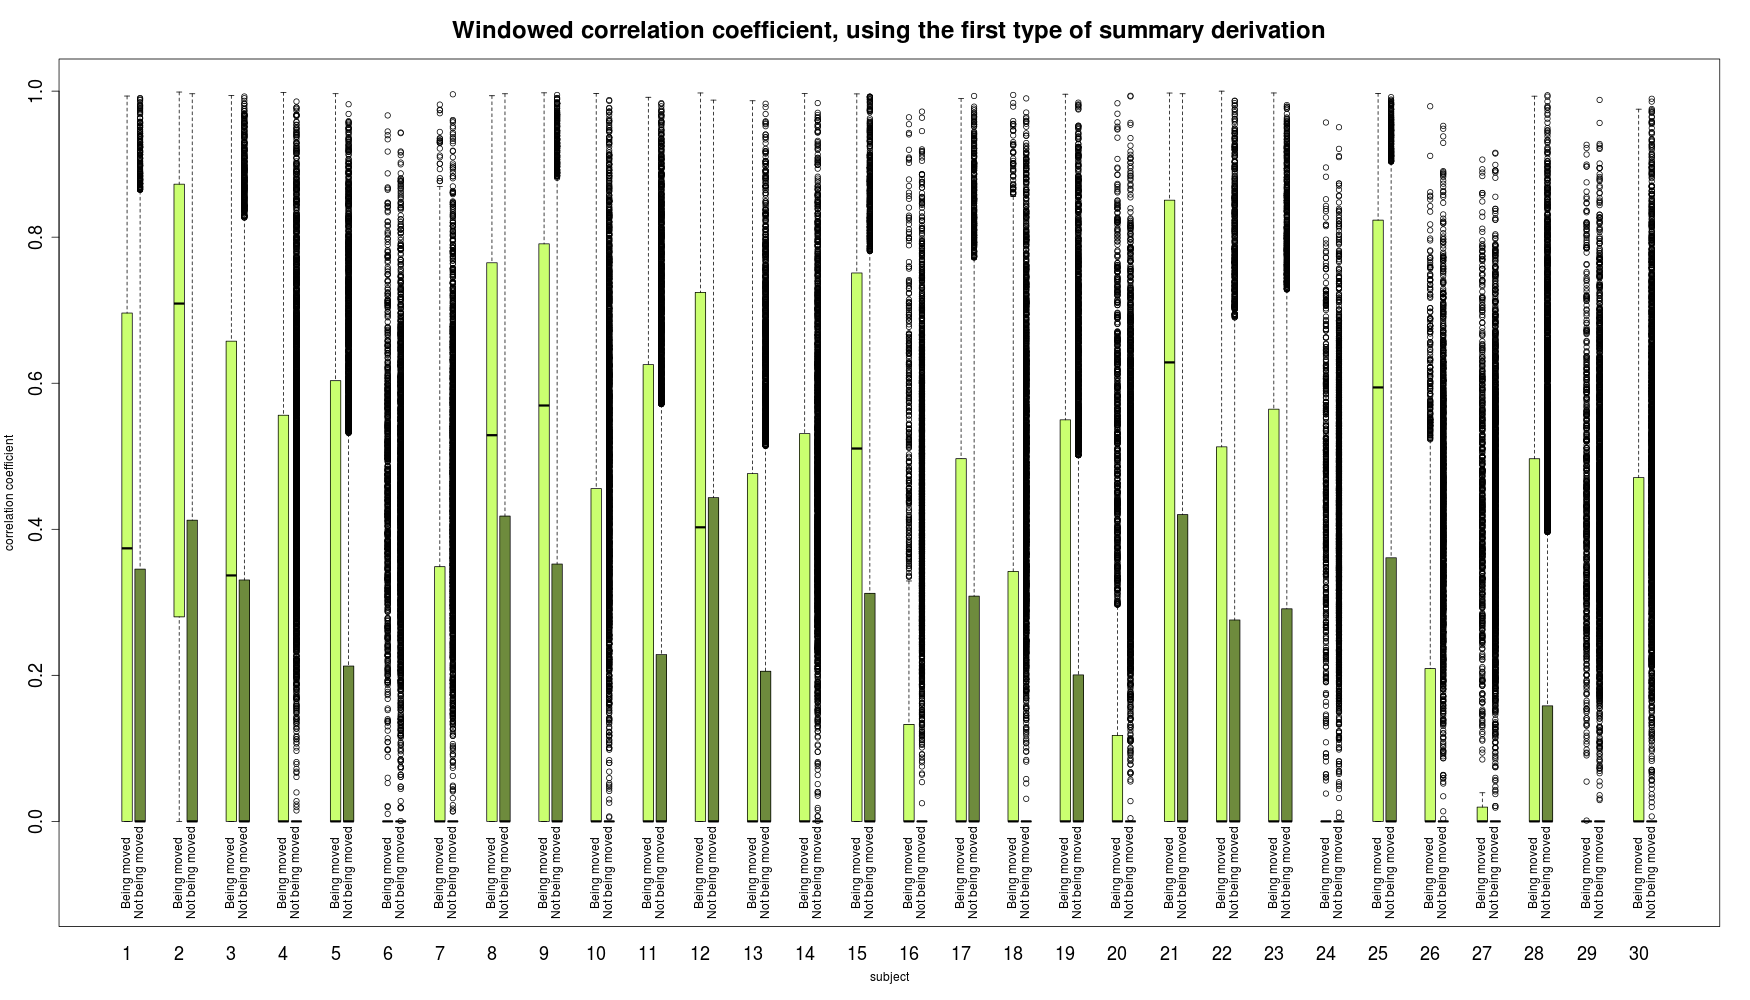
\includegraphics[width=15cm, height=8.5cm]{norm_result_being_moved_correlation_boxplot.png}
\caption{Absolute windowed correlation coefficient, grouped according to whether the infant was detected as being moved, using the first type of summary derivation.}
\end{figure}

\begin{figure}[h!]
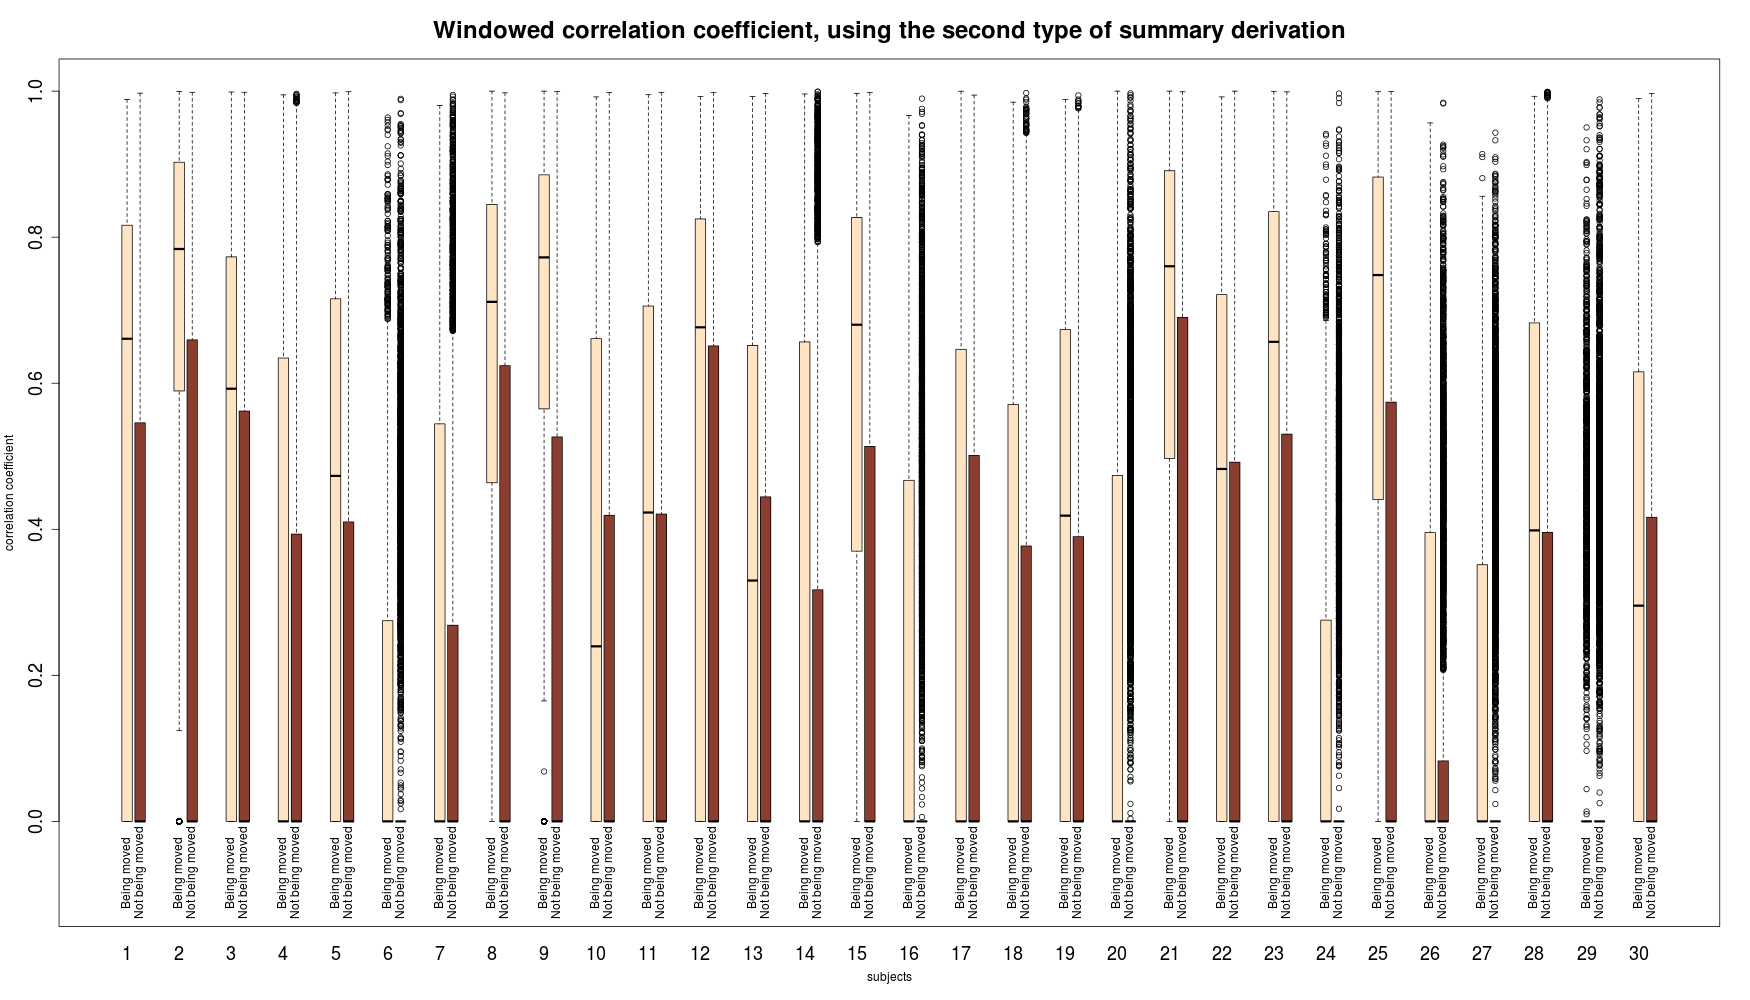
\includegraphics[width=15cm, height=8.5cm]{filter_result_being_moved_correlation_boxplot.png}
\caption{Absolute windowed correlation coefficient, grouped according to whether the infant was detected as being moved, using the second type of summary derivation.}
\end{figure}
\newpage

\begin{figure}[h!]
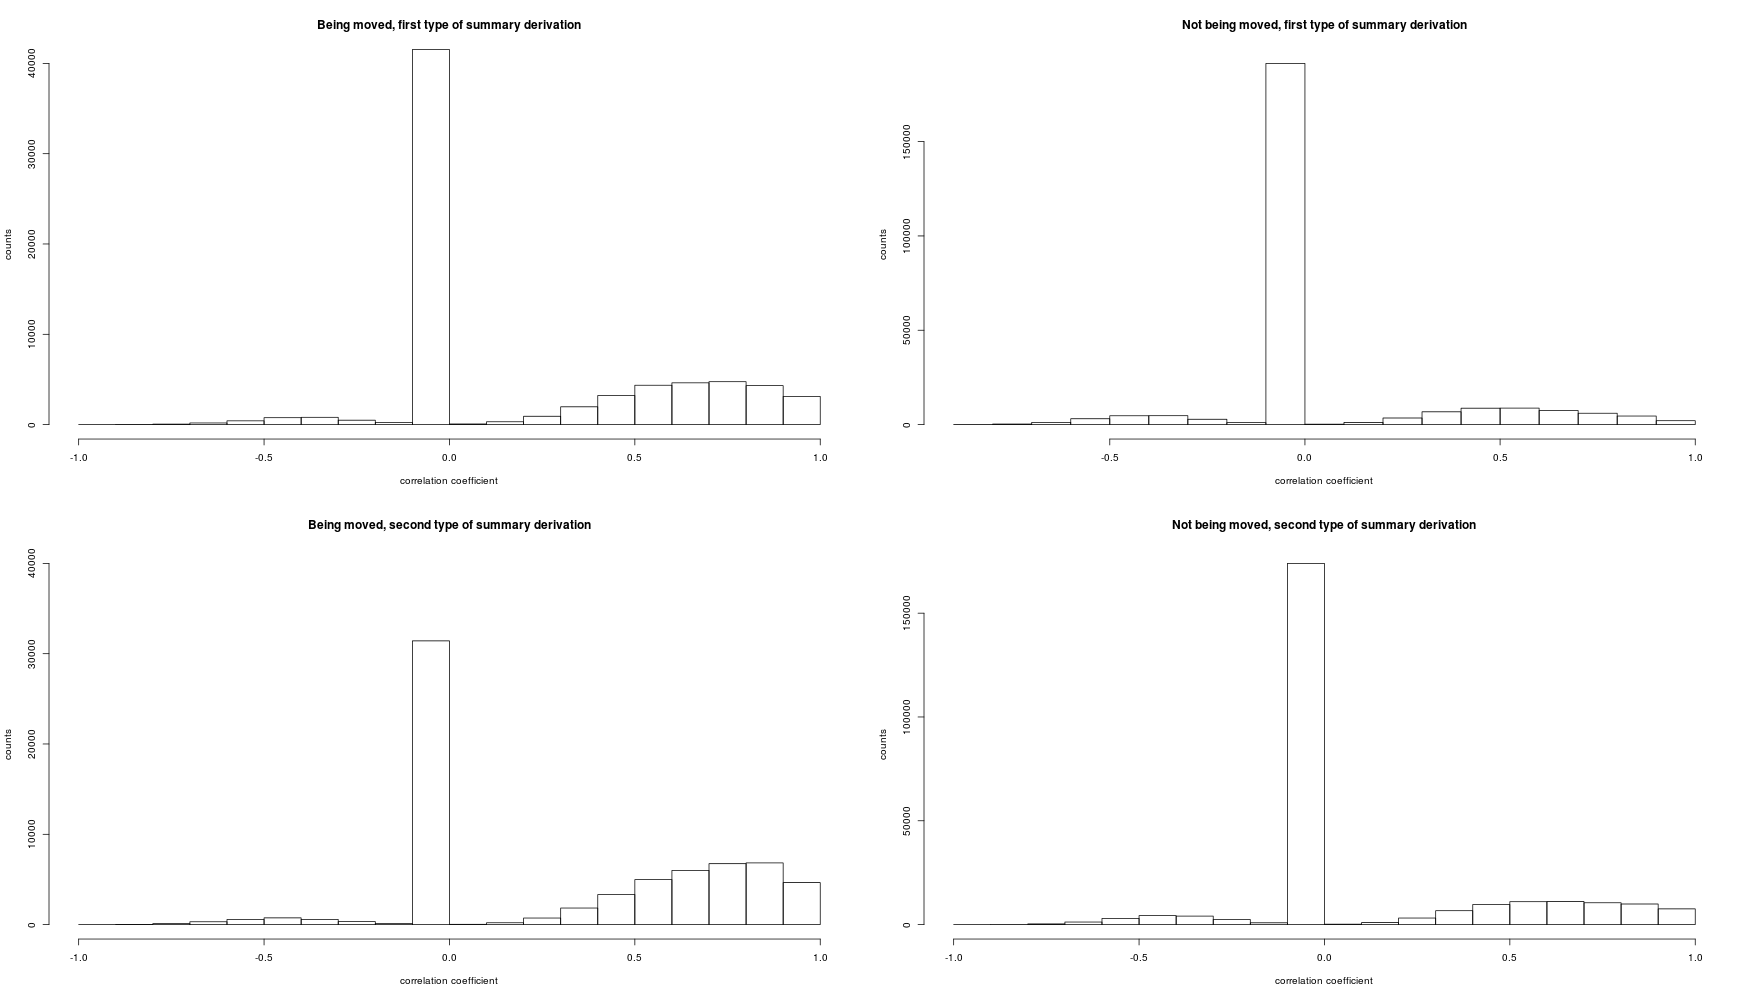
\includegraphics[width=15cm, height=8.5cm]{histogram_corr_coeff.png}
\caption{Distributions of the absolute windowed correlation coefficient, for the two types of summary derivation and the corresponding periods of infant being moved and not being moved.}
\end{figure}

\\Again, the second type of summary derivation has slightly better results. Mean absolute correlation coefficient of the periods where the infant was detected as being moved, results in 0.2660 and 0.3673 for the first and second type of summary derivation respectively. Since higher similarity might be due to better preservation of similarities in the accelerations contributed by the caretakers, the second type of summary derivation is chosen to be analyzed further. 
\\PA measure is extracted from the remaining or corrected ankle measurement and summarized with the second type of summary derivation. Two cut-points for the SD are used to extract levels of low PA and high PA. Based on trial and examination, cut-point for low PA was set to 0.03 g SD, while the cut-point for high PA was set to 0.05 g SD.
The proportion of time the infant is detected as active differs between the various approaches. One could already expect that extracting and analyzing PA based on the approach A will be meaningless, as the majority of accelerations present are still due to caretakers contributing accelerations. In fact, based on approach A and using the second summary derivation, the comparison between the infants low PA and being moved time, resulted in Spearmans rank correlation coefficient equal to 0.6301 with p-value < 0.0001, while the comparison between the infants high PA and being moved time, resulted in Spearmans rank correlation coefficient equal to 0.6463 with p-value < 0.0001, scatterplots shown in Figure 35.
\begin{figure}[h]
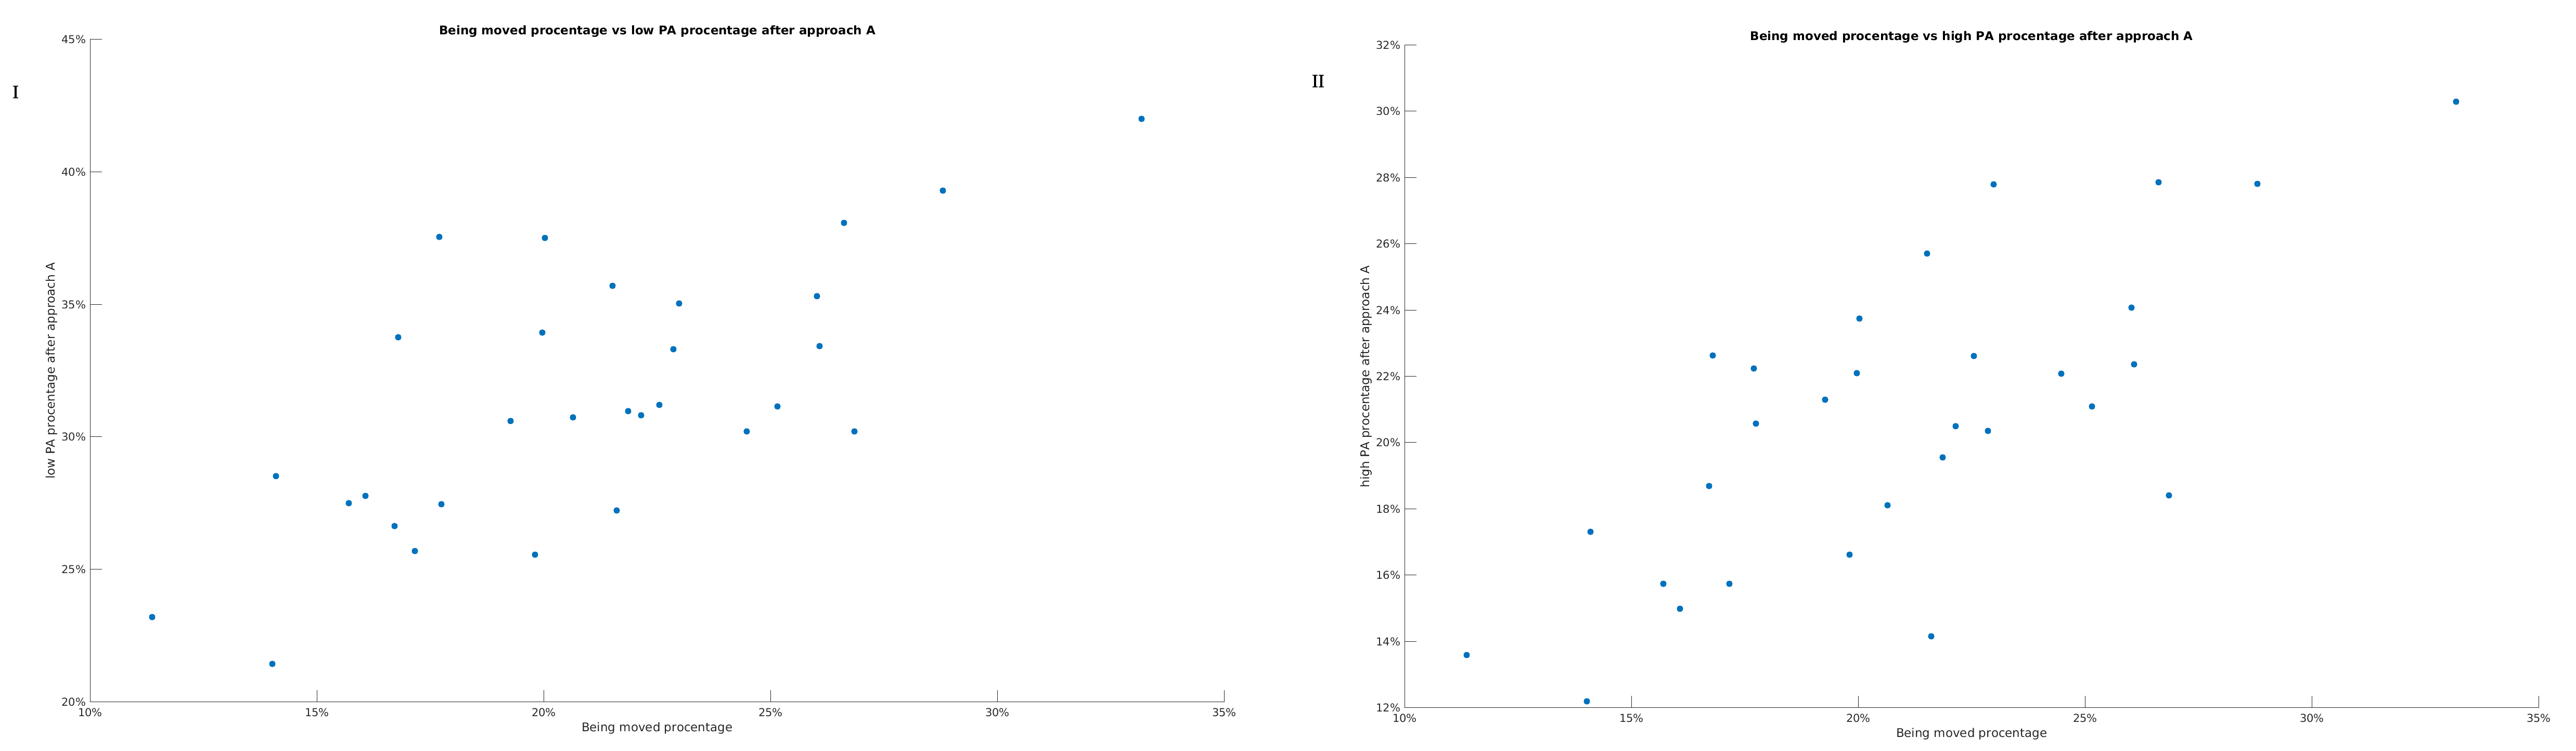
\includegraphics[width=15cm, height=6.5cm]{IBM_vs_PA_A.png}
\caption{Comparing the proportion of being moved time with infants low PA(I) and infants high PA(II), after approach \textbf{A} and using the second summary derivation.}
\end{figure}
\newpage
Results from correlation analysis of infants PA and being moved time in approach A make sense, as infants PA time and being moved time is extracted with the same procedure, using a slightly different SD cut-point. Considering this, along with the observation, that subtraction does not remove contributing accelerations, but in fact enhances them, it is not surprising these proportions end up being very similar. Infants PA measure, extracted after correction with the approach A would therefore substantially reflect the caretakers contributing accelerations and would therefore not be valid. Better results are expected where the subtraction is adjusted with the ratio between the accelerations of the torso and ankle placed measurements. For transparent comparisons, only approach \textbf{C} is analyzed, where the results from comparisons between the being moved time and infants low PA and high PA were non-significant, scatterplots shown in Figure 36. 
\newpage
\begin{figure}[h!]
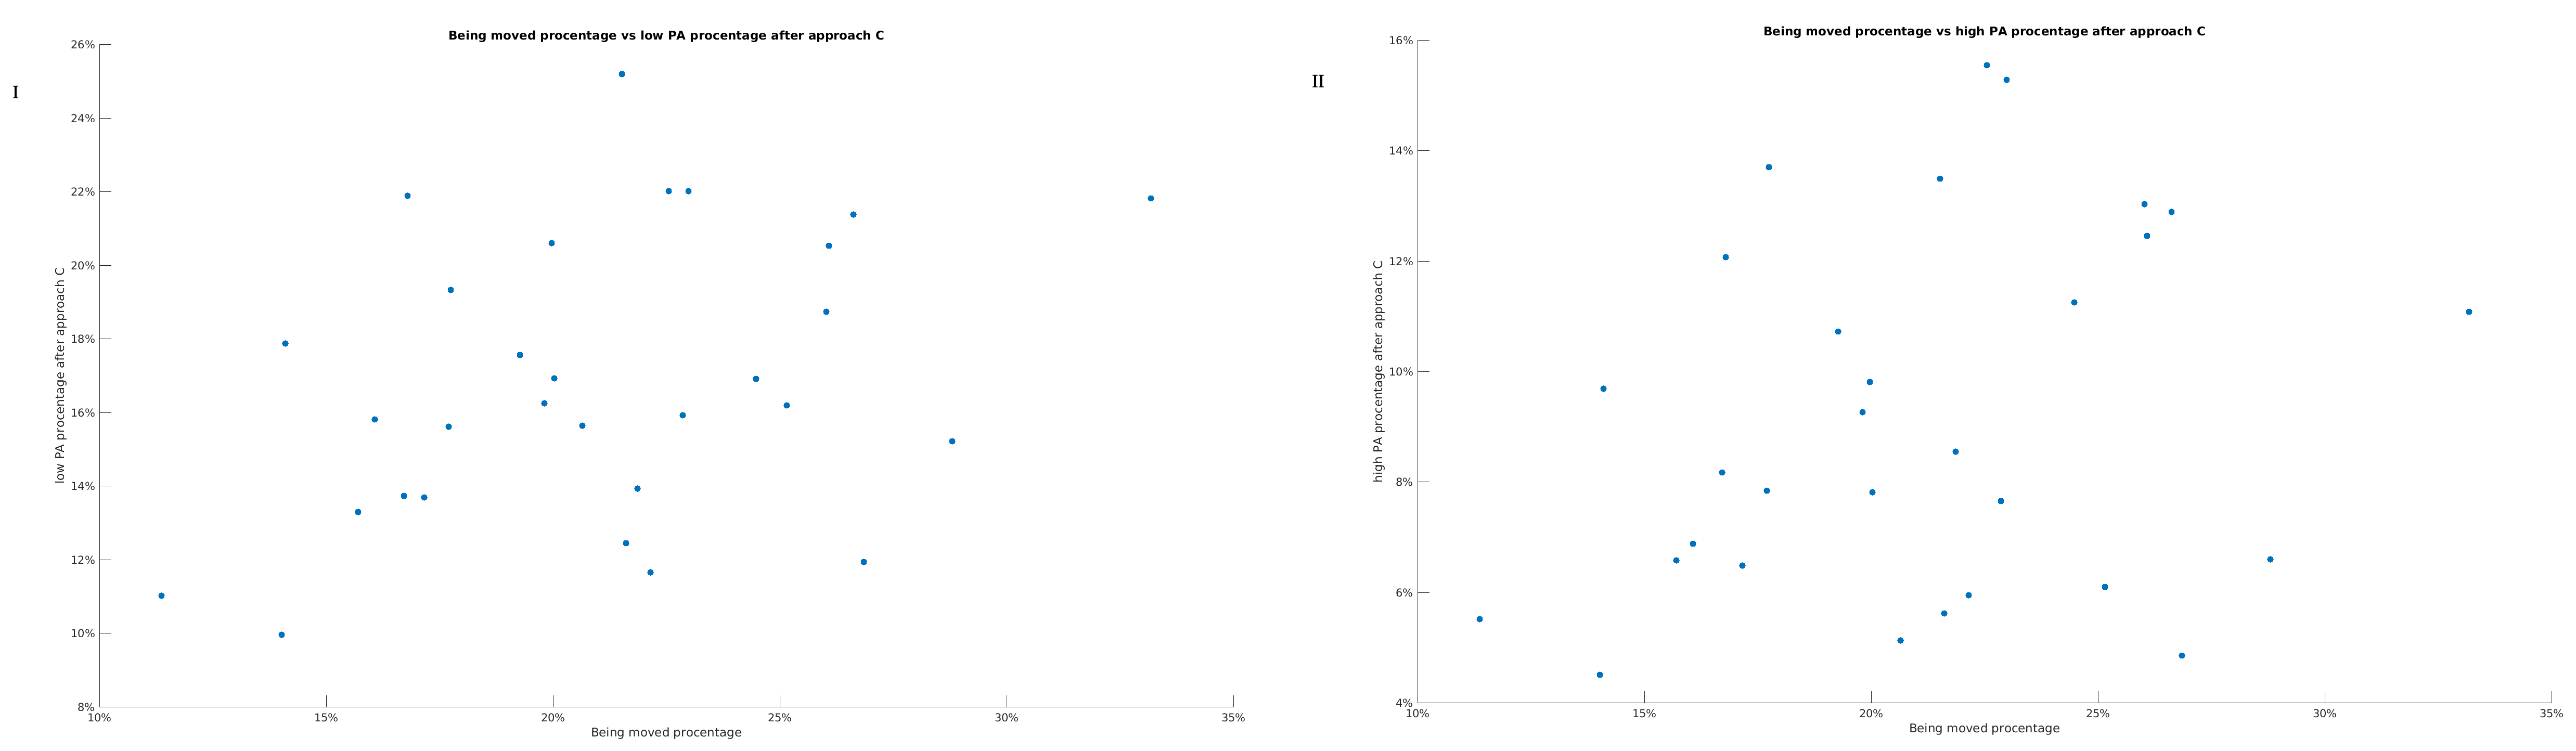
\includegraphics[width=15cm, height=6.5cm]{IBM_vs_PA_C.png}
\caption{Comparing the proportion of being moved time with infants low PA(I) and infants high PA(II), after approach \textbf{C} and using the second summary derivation.}
\end{figure}
\\\\\\
Results from the comparisons between the being moved time and infants low PA and high PA, based on approach \textbf{D}, were also non-significant, scatterplots shown in Figure 37. 
\begin{figure}[h!]
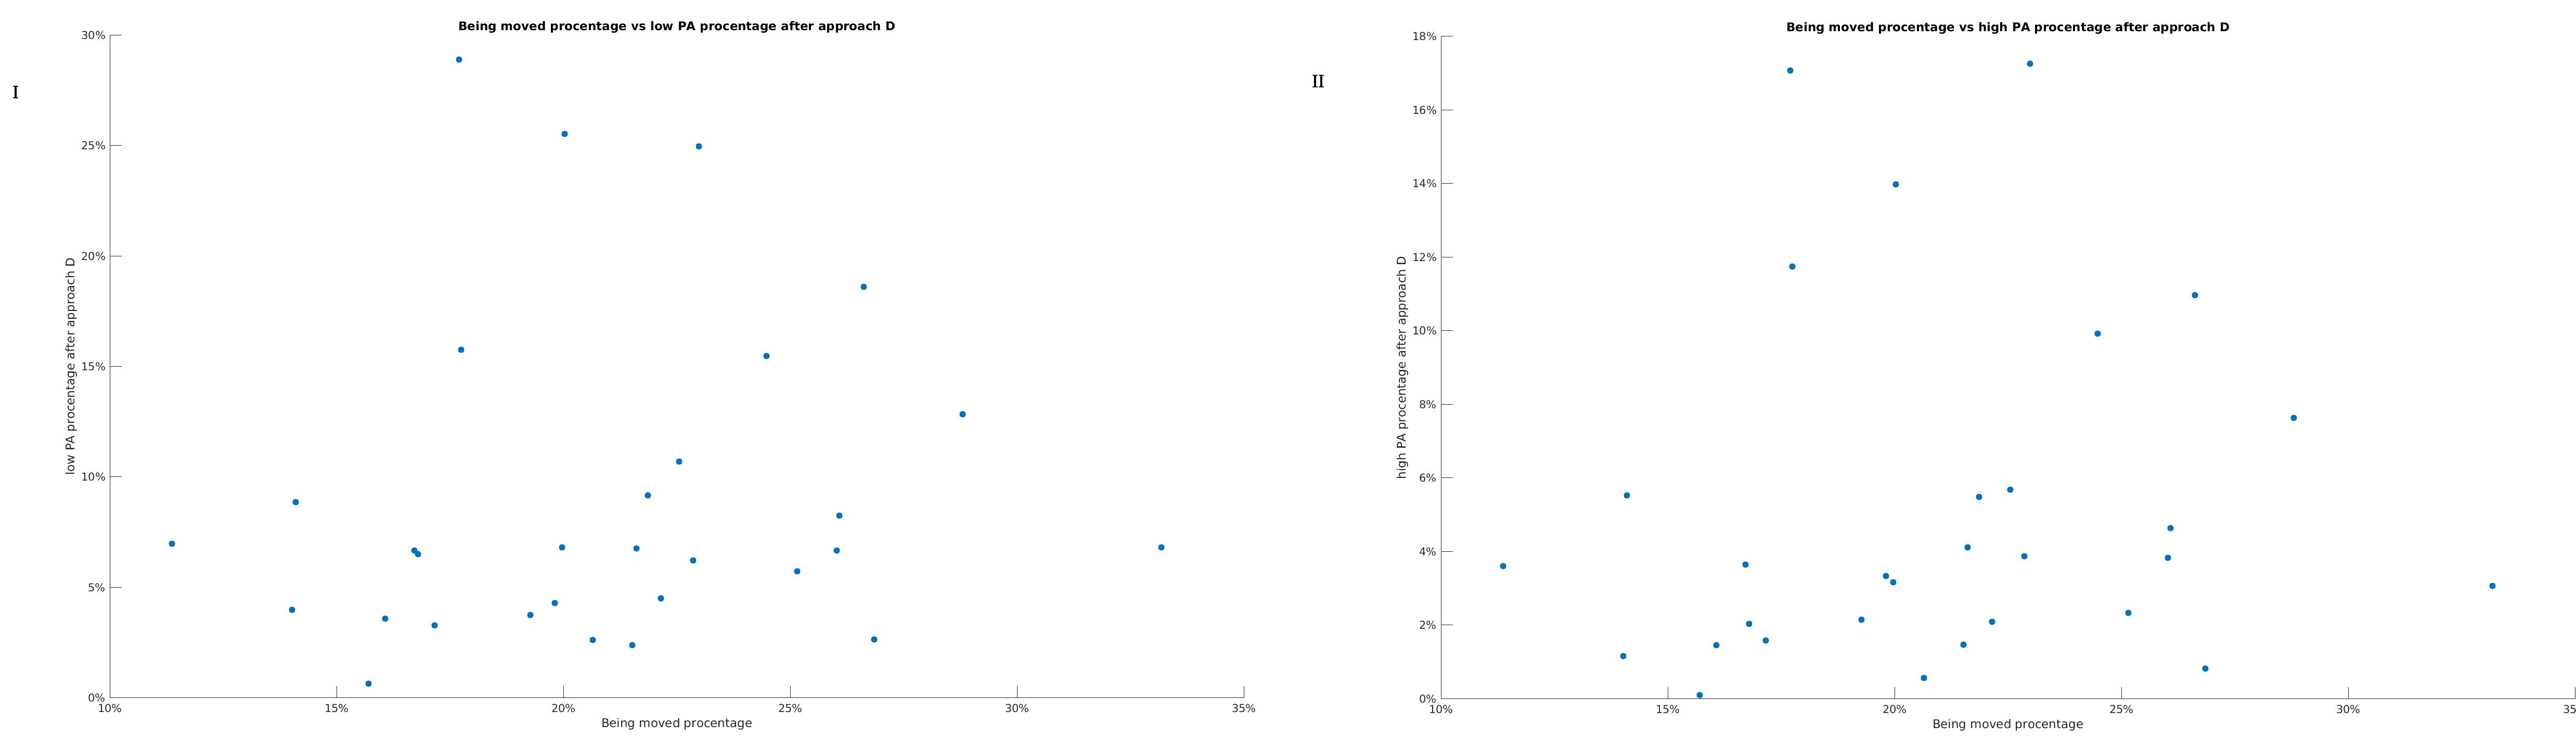
\includegraphics[width=15cm, height=6.5cm]{IBM_vs_PA_D.png}
\caption{Comparing the proportion of being moved time with infants low PA(I) and infants high PA(II), after approach \textbf{D} and using the second summary derivation.}
\end{figure}

Similar non-significant results were observed in approach \textbf{E}, scatterplots shown in Figure 38. 
 \begin{figure}[h!]
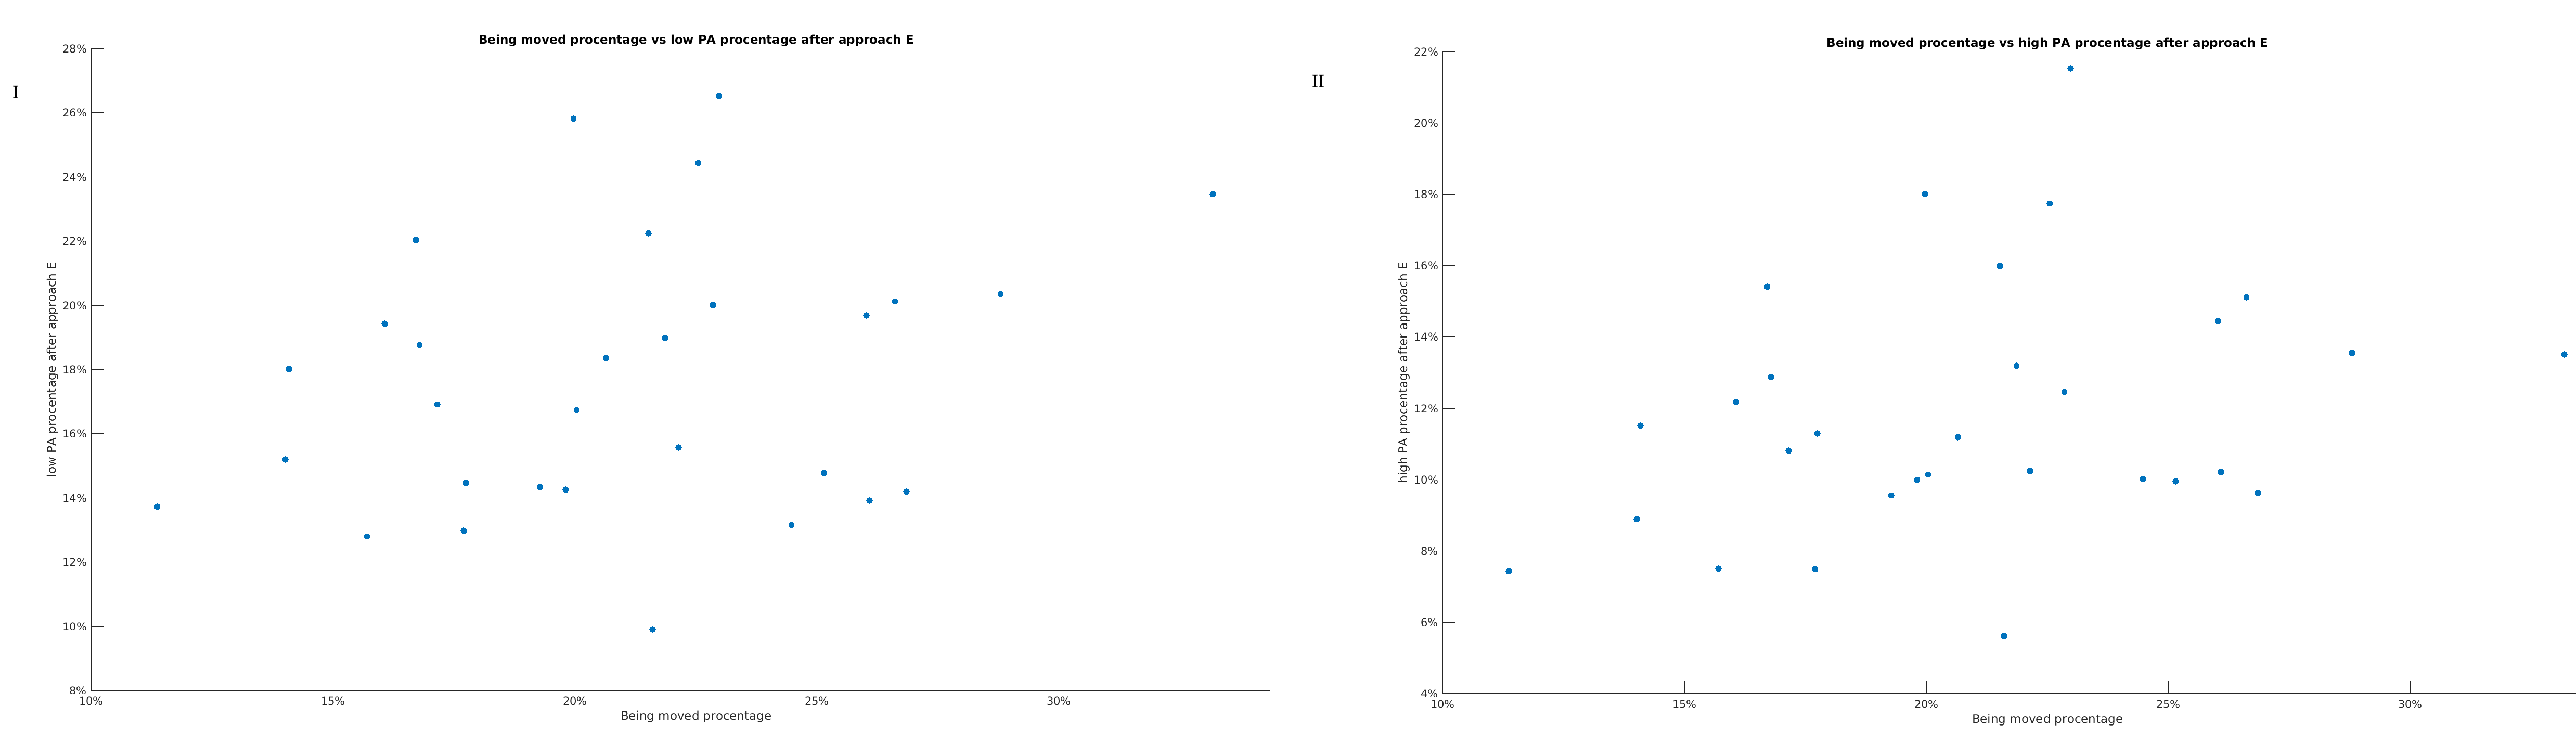
\includegraphics[width=15cm, height=6.5cm]{IBM_vs_PA_E.png}
\caption{Comparing the proportion of being moved time with infants low PA(I) and infants high PA(II), after approach \textbf{E} and using the second summary derivation.}
\end{figure}
\\

%------------------------------------------------

\subsection{Diary validation}

Outcomes of accelerometer data processing need to be validated. One possibility of validation was presented by the diaries of infants sleeping and feeding habits. The diaries could provide with information regarding the time of occurrences such as caretakers contributing accelerations or infants sleeping time, when less or no PA should be detected.
During the free living experiment, the mothers were instructed to keep a diary of infants feeding and sleeping habits, along with other valuable information regarding the experiment, like for example removal and reattachment of the accelerometer. All subjects had the diary data available, except one, where the diary was missing. The diary consisted of printed forms, example in Supplements. Besides a few exceptions, the mothers started keeping diary notations on the second day, from midnight on. This already presents a drawback, since the accelerometer data was recorded only for 48 hours from the morning of the first day on, meaning that out of those 48 hours, approximately 15 hours will not have corresponding diary notations. \\Since the diaries were filled by handwriting, the notations inside had to be digitized, to enable automatic comparison and validation. Although one could attempt to achieve this automatically by document scanning and image analysis, such approach would be too complicated and time-consuming for the needs of this project, where only 30 documents had to processed. Therefor these documents were examined manually, which was nevertheless still very time consuming and error prone. For several reasons, a substantial amount of error was also introduced by the mothers keeping the notations. Mainly this was due to rounding up the noted time, having trouble keeping up with notations and then not being able to recall the time of certain occurrences.\\
\\First, the diary forms enabled notation of accelerometer removal and reattachment, where the mothers had to note which of the accelerometers is being taken off, corresponding comments and the absolute time of removal and reattachment. Frequently, the mothers commented that the accelerometer was forgotten to be put back on after removal and the times noted are therefor approximate. Secondly, the diary forms included a schedule over 24 hours, over a week, where the mothers were instructed to note the infants sleeping time with a stroke. As one can see in the Supplements, the sleeping schedule is not so big, meaning that the space for one hour is very small. Consequently, it was difficult for the mothers to keep accurate and consistent notations of infants sleeping time. The noted times became even less accurate, when the mothers forgot to note regularly and had to therefor recall the approximate times of sleeping. For the validation and comparison of data analysis, absolute timestamps are needed and had to be therefor created manually, by examining these schedules, which introduced even more error. The final timestamps are therefor liable to be very approximate and error prone and one should begin to question whether comparison and validation against such timestamps is useful and valid itself. \\Last, mothers were instructed to keep a diary of infants feeding time, by noting down the begin time and duration of feeding, along with a few other comments, not relevant for this project. Feeding notations had to be transformed into begin and end timestamps, to enable validation and comparison. Example of the final data table, created manually based on a diary, in Table 2.\\

\begin{table}[h]\tiny
\begin{tabular}{|l|l|l|l|l|l|}
\hline
feeding start  & feeding finish & sleeping start & sleeping finish  & torso accelerometer detached & torso accelerometer reattached \\ \hline
2009-02-10 08:20:00 & 2009-02-10 08:50:00 & 2009-02-10 00:00:00 & 2009-02-10 08:10:00 & 2009-02-09 11:30:00 & 2009-02-09 16:00:00 \\ \hline
2009-02-10 09:30:00 & 2009-02-10 10:00:00 & 2009-02-10 13:00:00 & 2009-02-10 13:40:00 & 2009-02-09 18:30:00 & 2009-02-09 20:00:00 \\ \hline
2009-02-10 10:00:00 & 2009-02-10 11:00:00 & 2009-02-10 15:00:00 & 2009-02-10 15:25:00 & 2009-02-10 21:10:00 & 2009-02-11 08:15:00 \\ \hline
2009-02-10 14:15:00 & 2009-02-10 15:00:00 & 2009-02-10 19:00:00 & 2009-02-10 19:40:00 &    &    \\ \hline
2009-02-10 15:50:00 & 2009-02-10 16:20:00 & 2009-02-10 22:20:00 & 2009-02-11 08:25:00 &    &    \\ \hline
2009-02-10 17:30:00 & 2009-02-10 17:45:00 & 2009-02-11 10:30:00 & 2009-02-11 11:40:00 &    &    \\ \hline
2009-02-10 20:00:00 & 2009-02-10 20:30:00 & 2009-02-11 13:25:00 & 2009-02-11 14:00:00 &    &    \\ \hline
2009-02-10 21:00:00 & 2009-02-10 21:15:00 & 2009-02-11 19:30:00 & 2009-02-11 20:05:00 &    &    \\ \hline
2009-02-11 08:20:00 & 2009-02-11 09:30:00 & 2009-02-11 22:00:00 & 2009-02-12 08:25:00 &    &    \\ \hline
2009-02-11 11:30:00 & 2009-02-11 11:45:00 &    &    &    &    \\ \hline
2009-02-11 14:15:00 & 2009-02-11 15:00:00 &    &    &    &    \\ \hline
2009-02-11 15:00:00 & 2009-02-11 16:00:00 &    &    &    &    \\ \hline
2009-02-11 16:50:00 & 2009-02-11 17:15:00 &    &    &    &    \\ \hline
2009-02-11 17:30:00 & 2009-02-11 17:45:00 &    &    &    &    \\ \hline
2009-02-11 19:15:00 & 2009-02-11 19:35:00 &    &    &    &    \\ \hline
2009-02-11 20:30:00 & 2009-02-11 21:00:00 &    &    &    &    \\ \hline
2009-02-11 21:15:00 & 2009-02-11 21:30:00 &    &    &    &    \\ \hline
\end{tabular}
\caption{Example of a data table, created manually based on a diary kept by the infants mother.}
\end{table}
Overall, the handwritten diaries were hard to examine, due to unclear handwriting and sloppy notes which often did not make sense. It became likely that the diaries will not provide the desired means for validation, especially if considering the amount of error along with the frequency of feeding and sleeping occurrences. Nevertheless, the diary timestamps are compared against the timestamps obtained through data analysis in an attempt to extract any kind of validating information. \\
\\First, timestamps obtained through automatic non-wear time detection are compared to the timestamps generated based on the diaries. The comparison is implemented in Python, with the help of modules \textit{pandas}, \textit{datetime} and \textit{dateutil}. Even though the exact time of the beginning and end of non-wear occurrences differed between the timestamps for an average of one hour, all the major non-wear occurrences are detected, with a few exceptions of either very short non-wear occurrences or occurrences where the accelerometer was noted as not being worn, but the measurement clearly showed movement. Based on the visual examination of plots with no-wear time marked, the time-stamp differences are due to the errors in the diary based timestamps and not in the data analysis.
\\Second, the timestamps obtained through detection of infant being moved and the timestamps obtained through detection of infants PA are compared to the sleeping and feeding blocks noted in the diary. Ideally one would expect to have caretakers contributing accelerations detected around the begin and end of sleeping blocks and all through out from begin to end of a feeding block, while there should be less caretakers contributing accelerations detected, while the infant is sleeping, when there should also be substantially less infants PA. Considering the amount of error introduced with the diaries and the frequency of sleeping and feeding occurrences, it would be uninformative to compare the exact timestamps and their differences, instead, for all detected timestamps of caretakers contributing accelerations, proportions of time are calculated regarding into which diary block the timestamps fell.\\Altogether, nine blocks are defined. A block of time where the infant was sleeping and feeding, sleeping only, feeding only, close/around of a sleeping and feeding block, close/around to sleeping only block, close/around to feeding only block, inside of a sleeping block, but also being close/around a feeding block, inside of a feeding block, but also being close/around a sleeping block and the final block being none of the above, meaning infants free awake time. Final proportions overall subjects in Table 3.
\begin{table}[h]\tiny
\centering
\begin{tabular}{|p{0.5cm}|p{1cm}|p{1cm}|p{1cm}|p{1.5cm}|p{1.5cm}|p{1.5cm}|p{1.2cm}|p{1cm}|p{1cm}|p{1cm}|p{1cm}|p{1cm}|}
\hline
overall subjects & inside of a sleeping and feeding block & inside of a sleeping block only & inside of a feeding block only & close to start or end of a sleeping and feeding block & inside of a sleeping block but also close to the start or end of a feeding block & inside of a feeding block but also close to the start or end of a sleeping block & close to start or end of a sleeping block only & close to start or end of a feeding block only & not in or near feeding or sleeping block \\ \hline
mean & 0.82\% & 40.73\% & 3.31\% & 2.86\% & 3.15\% & 0.61\% & 15.87\% & 5.18\% & 27.42\% \\ \hline
min & 0\% & 9.40\% & 0\% & 0\% & 0\% & 0\% & 7.84\% & 0.44\% & 12.03\% \\ \hline
max & 6.59\% & 60.56\% & 29.37\% & 7.22\% & 10.53\% & 3.92\% & 25.04\% & 17.36\% & 43.94\% \\ \hline
SD & 1.65\% & 24.04\% & 3.31\% & 1.89\% & 3.08\% & 0.91\% & 4.79\% & 3.75\% & 9.42\% \\ \hline
\end{tabular}
\caption{Table of time-stamp proportions falling in certain diary blocks. }
\end{table}
\\
The biggest proportions are represented by the sleeping block only and infants free awake time, although the SD is very high with both. On average, SD is very high for all the defined blocks and the span between minimum and maximum is large, showing a substantial amount of variability between the subjects. In figures 39 and 40, examples of plots where the measurement is noted with detected caretakers contributions, sleeping and feeding blocks and night time, show the variability and the frequency of different occurrences, resulting in less informative validation. For more accurate results, the amount of day and night time should be taken into account as well, since the accelerometer data lacks 15 hours of diary data and the rest of the 33 hours will have two nights and only one day, which results in more sleeping time.
\begin{figure}[h!]
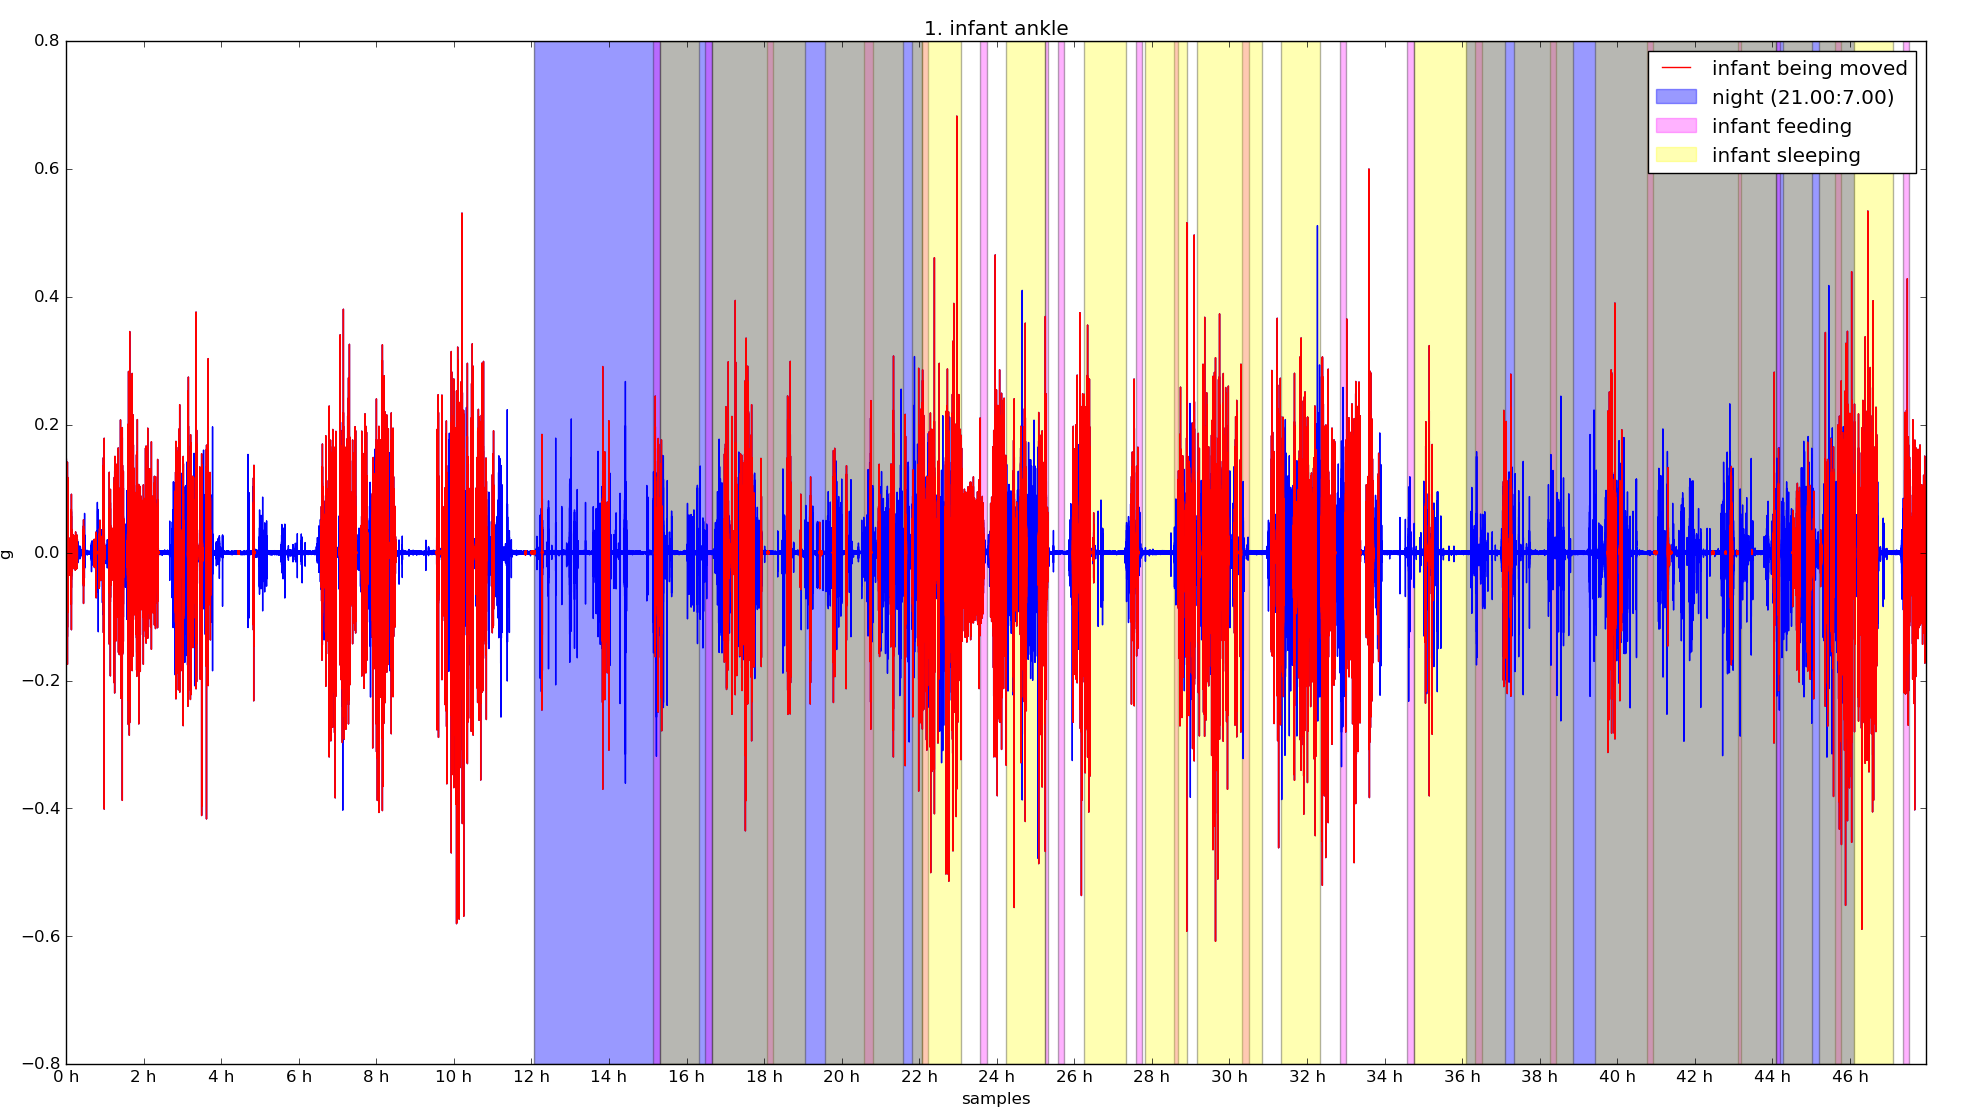
\includegraphics[width=15cm, height=6cm]{1moved.png}
\caption{The sleeping and feeding occurs in short blocks all through the experiment, night time is less expressed. }
\end{figure}

\begin{figure}[h!]
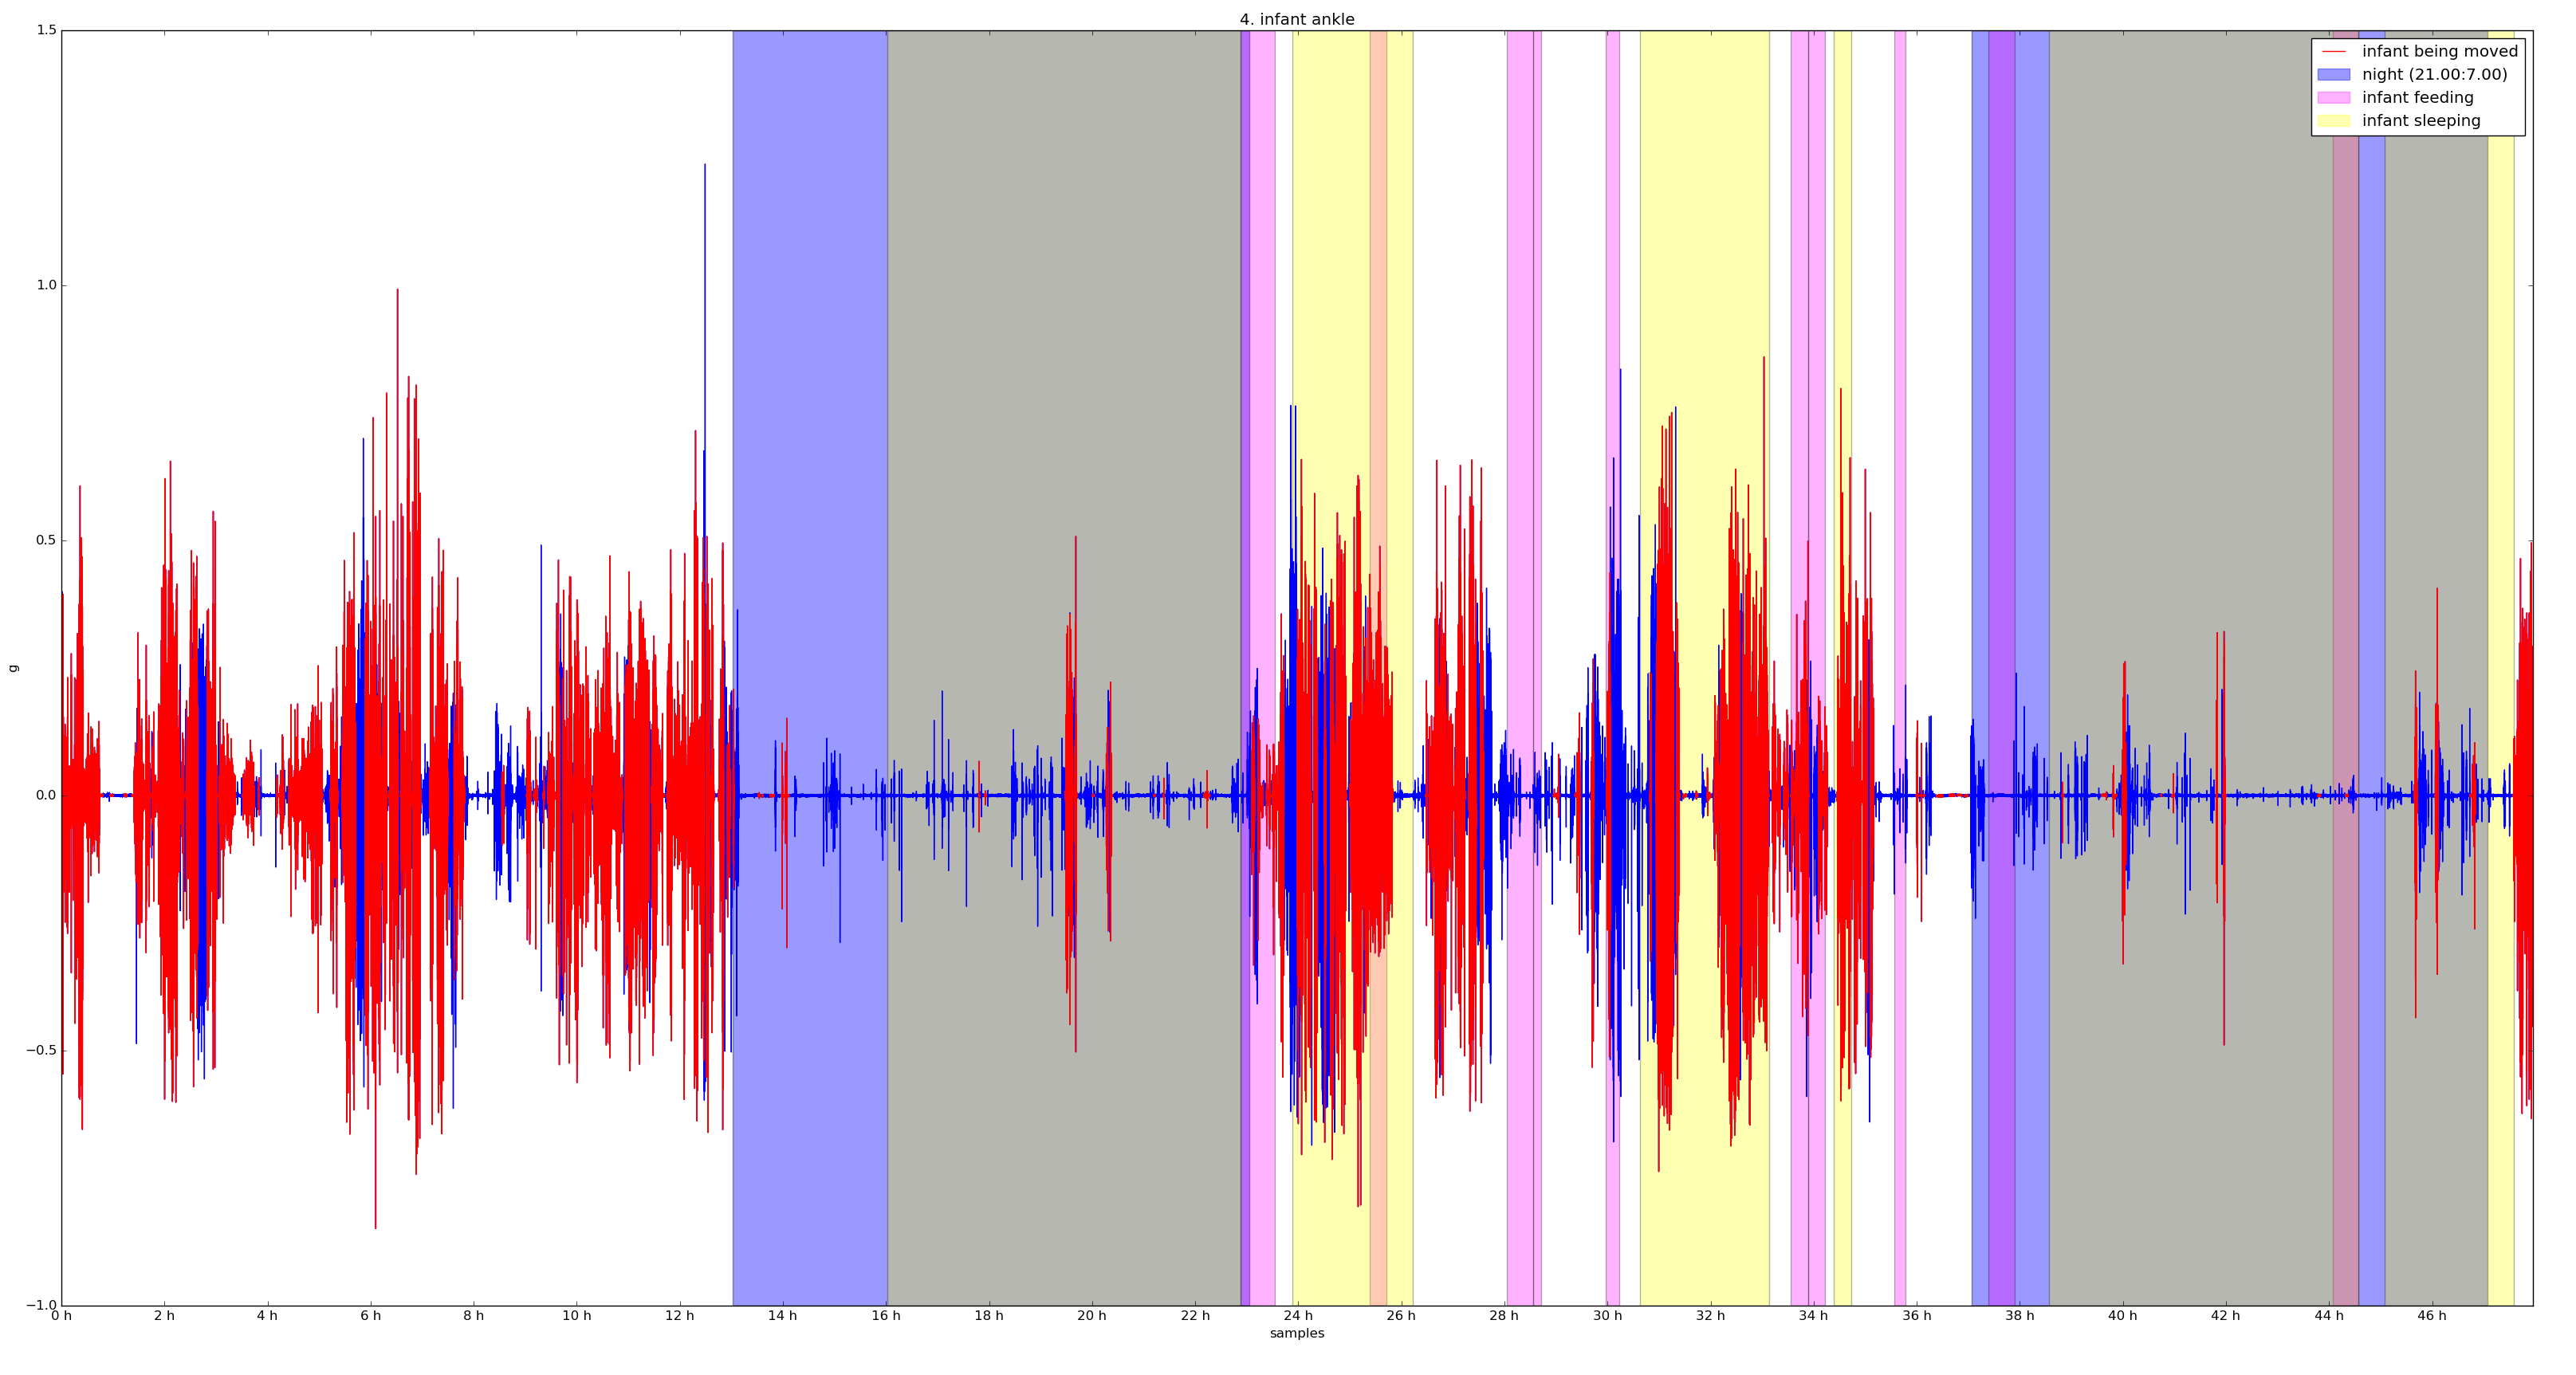
\includegraphics[width=15cm, height=7cm]{4moved.png}
\caption{The sleeping and feeding occurs in larger blocks, night time is more expressed with clearly less caretakers contributions detected.}
\end{figure}
Evidently, the diaries are not precise enough to validate the detection and correction of the contributing accelerations. Nevertheless, the extracted proportion of PA can be compared against the sleeping and awake blocks, in order to compare the amount of PA during sleeping and during awake time. Table 4 presents the proportion of time the extracted PA occurred while infant awake time.\\

\begin{table}[h!]
\centering
\label{my-label}
\begin{tabular}{|c|c|c|c|c|c|c|}
\hline
\multirow{2}{}{} & \multicolumn{2}{c|}{\textbf{approach C}} & \multicolumn{2}{c|}{\textbf{approach D}} & \multicolumn{2}{c|}{\textbf{approach E}} \\ \cline{2-7} 
 & low PA & high PA & low PA & high PA & low PA & high PA \\ \hline
mean & 40.17\% & 40.63\% & 44.82\% & 47.90\% & 40.93\% & 40.15\% \\ \hline
SD & 12.22\% & 15.40\% & 20.78\% & 26.75\% & 12.37\% & 13.58\% \\ \hline
min & 19.22\% & 17.24\% & 10.54\% & 0\% & 13.16\% & 12.26\% \\ \hline
max & 61.98\% & 70.95\% & 88.63\% & 100\% & 60.23\% & 60.62\% \\ \hline
\end{tabular}
\caption{Proportions of PA occurring while infant awake, after different approaches.}
\end{table}
\newpage
In all approaches, the average proportion of PA occurring while infant sleeping is larger then expected, although the SD of the proportions is again very high, as is the span between the minimum and maximum and most importantly, the outcomes might not be accurate, since as previously mentioned, normalization with the total sleeping and awake time should have been done. Infants at four months of age tend to sleep most of the time, which will already result in bias towards sleeping time, descriptive statistics of feeding and sleeping time extracted from the diaries in Table 5. 
\begin{table}[h!]
\centering
\begin{tabular}{|l|l|l|}
\hline
over all subjects & sleeping time & feeding time \\ \hline
mean   & 63.00\%  & 9.63\%  \\ \hline
min   & 38.99\%  & 3.30\%  \\ \hline
max   & 81.60\%  & 27.01\% \\ \hline
SD   & 9.39\%  & 6.01\%  \\ \hline
\end{tabular}
\caption{Proportion of sleeping and feeding time overall subjects with a diary available.}
\end{table}
\\Validation with two nights and one day of dairy data will only increase the bias towards sleeping time and so might the correction or removal of the periods when the infant was being moved, since the infant could have been carried around most of time being awake, example in Figure 41.
 \begin{figure}[h!]
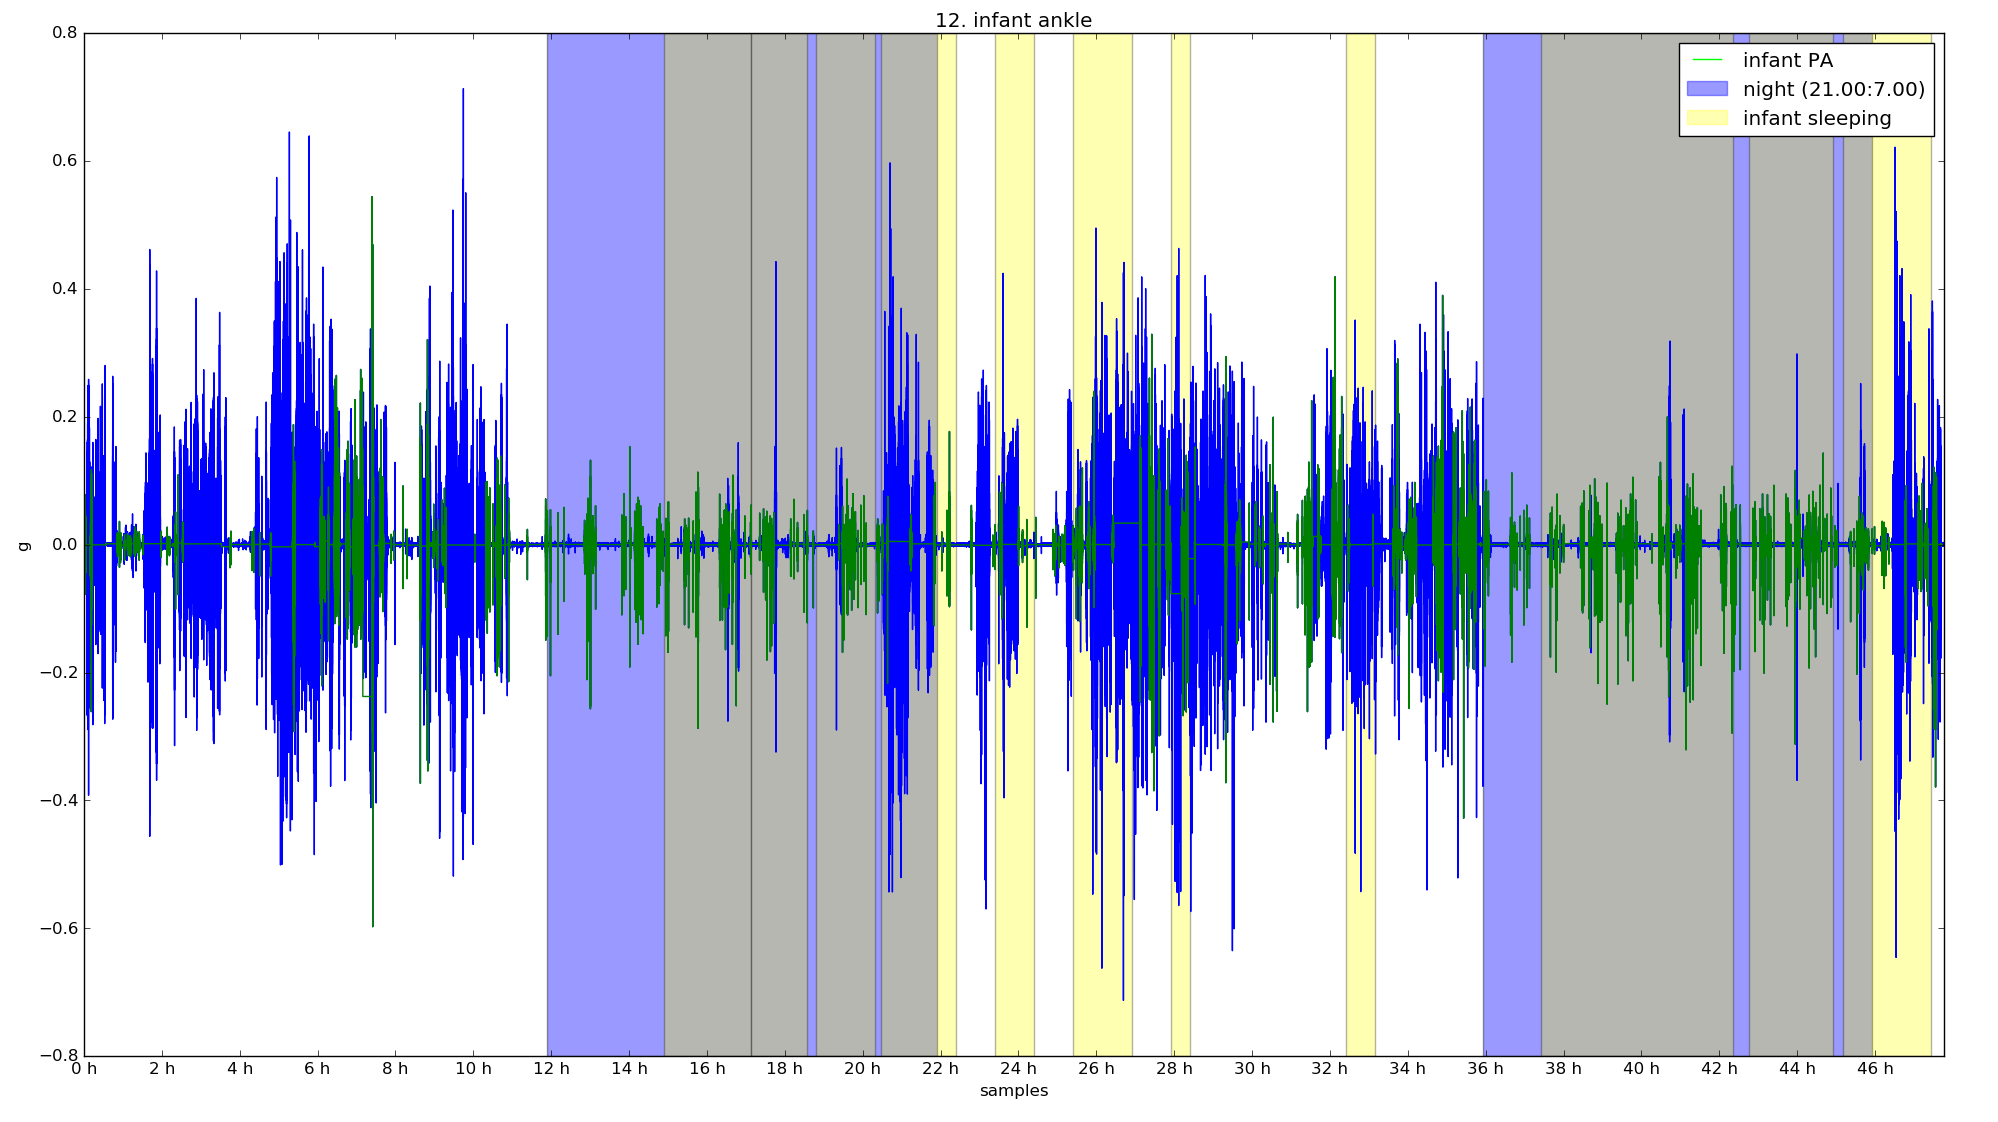
\includegraphics[width=15cm, height=7cm]{12PA.png}
\caption{Example of the extracted PA along with the diary noted sleep and night time according to the absolute time-stamp.}
\end{figure}
\\Overall, the validation against the diaries did not provide the desired and planed validation. With the high frequency of daily sleeping and feeding occurrences, the amount of error present in the diaries and introduced with digitization is exceedingly high, while the infants time is biased to sleeping. 
}

\newpage
\section{Closure}
\fontsize{11.25pt}{11.1pt}\selectfont {

\subsection{Discussion}
Aim of the current project was to process and analyze accelerometer data taken of four month old infants, in order to extract a measure of infants PA and assess the validity and feasibility of the extraction.
\\\\Accelerometer data analysis is challenging, despite the common use of accelerometers for PA estimation. Complications arise as of first step of processing by the summary derivation. The choice and derivation of the summary has turned out to be a non-trivial step, which decreases the feasibility of infants PA measure extraction. Reasons are the lack of established consensus regarding an optimal summary derivation, accompanied with large amount of published methods and researches, where the commonly used summary derivations are fundamentally different. Further more, the outcome of the summary derivation is heavily dependent on the filtering parameters and window size, which should be set in consideration of the accelerometer brand, accelerometer settings and the subject wearing the accelerometer. There are several published researches addressing these parameters for the accelerometer used in the current project (GENEA), but none for infants. This led to trial and examination based settings of parameters, resulting in uncertain and error prone outcomes. This might have been avoided or improved by ensuring a well defined training dataset, obtained by laboratory based observations of movements and their corresponding recorded accelerations. 
\newpage
Training data would have also aided in the very important step of correction of caretakers contributing accelerations. Without appropriate correction, infants PA measure would reflect caretakers contributing accelerations. In 2009, a paper titled \textit{Mechanical Measurement of Infant Activity: A Cautionary Note} \cite{ref1} was published. The main message of the paper was that much of infants measured activity may be confounded by their caretakers contributions. An experiment was performed as a basis for the paper, where a mother and her 3 month old infant had a normal 24 hour day with usual activities, while a researcher with a motionless doll would mimic everything the mother did with her infant. Both the infant and the doll wore motion loggers on the chest and ankle. The results were then analyzed and compared. As one would expect, the dolls measurement showed a substantial amount of activity which would normally be unusual for a motionless doll. When comparing infants activity levels to the ones of the doll, approximately 45\% more activity was detected, meaning that the monitor will pick up both, the infants and caretakers contributions. Without a well defined training data present, it is left to advanced analysis to distinguish between the contributed accelerations and accelerations due to infants PA. In 2014 a PhD thesis was submitted, titled \textit{Physical activity in infancy: assessment of an intervention to increase physical activity in infants}\cite{ref6}. As part of the research, the defended studied and analyzed the feasibility to assess PA in 6-month old infants using an accelerometer, based on a validation study performed in 2012, with the results available in a conference abstract\cite{ref5}. The goal of the study was to assess the degree of caregiver confounding that might be expected in these measurements. Similar to before \cite{ref1}, the infants and motionless dolls wore three accelerometers, one on the wrist, one on the ankle and one on the waist. While the caretaker would perform several activities with the infant, the research assistant would mimic their actions with the doll. Overall 34 mother-infant pairs participated, although some did not perform all the activities. The results showed that when the infant is pushed in a stroller, 29\% of the arm movement and 9\% of the leg movement is due to contributing accelerations, while when being carried, contributing accelerations add up to 23\% of the arm movement and 52\% of the leg movement. With another type of activity with a Swiss ball, 28\% of the arm movement and 21\% of the leg movement was due to contributing accelerations. For all activities, the waist accelerometer recorded more activity on the doll rather then the infant, which resulted in an invalid measurement. An interesting observation showed that the overall output differed significantly between the three differently placed accelerometers, when in fact recording the \textit{same} activity. Overall, the study\cite{ref5} showed that up to half of the detected activity can be due to contributing accelerations, while these contributions differ significantly between the activities performed and between the differently placed monitors, as well as between the caretakers.\\\\
Similar results were observed in the current project. Caretakers contributing accelerations were estimated based on increased acceleration on the torso placed accelerometer and occurred up to 35\% of total measurement time. In the most ineffective correction method, the extracted PA measure was highly and significantly correlated with the measure of caretakers contributing accelerations, illustrating the invalidity of the uncorrected PA measure. Clear similarities between the torso and ankle placed measurement were observed on a large scale, indicating caretakers contributing accelerations, while more accurate observations revealed substantial differences on a smaller scale. Differently placed accelerometers can record different accelerations for the \textit{same} activity carried out by the caretaker, while also recording infants own accelerations specific to a certain body part, making it hard to distinguish between the sources of accelerations. With such issues one can resort to complete removal of periods when caretakers contributing accelerations were detected. This might be a feasible solution with a sufficient amount of data, but in 48 hours of measurement, there is little left after such correction, while the remaining measurement is biased towards infants sleeping time.
\\\\In the end, the extracted PA measure has to be validated. The hand written diaries do not provide the appropriate and necessary means of validation. Infants require care with a high frequency, while care taking is often demanding and stressful, leaving the caretaker preoccupied to keep up with the sufficiently accurate notes.

\subsection{Conclusions}
The torso and ankle placed measurements contain recordings of increased accelerations with a substantial amount of similarity on a large scale, which indicates caretakers contributing accelerations. The overall presence of similarity and the amount of blocks with highly increased SD of the torso placed measurement, correspond to the previous reports regarding confounding accelerations due to infants caretaker \cite{ref1}\cite{ref5}\cite{ref6}. High variability present between the subjects and differently placed accelerometers is also observed as in previous reports. To enable a valid extraction of infants PA, the contributing accelerations need to be removed. Based on the approaches developed and explored in this project, one has to consider:
\begin{itemize}
\item There is a substantial amount of difference between the torso and ankle placed measurements on a local scale, therefor a good enough summary of the measurement has to be derived,
\item Besides the local differences, the torso placed measurement is not necessary smaller then the ankle placed one, so simple subtracting will result in impaired further analysis,
\item Extracting signal similarities could be a potentially good approach to correct contributing accelerations,
\item Removing all the periods, when caretakers contributing accelerations are detected, results in substantially less measurement, measurement biased to sleeping time, which might interfere with the extraction of PA,
\item Appropriate and valid means of validation need to be obtained, where one should not rely on the caretaker to provide them.
\item Extraction and validation of infants PA measure from accelerometer data is a highly demanding task and remains unfeasible without an appropriate experiment design and advanced signal processing methods, preferably with a well defined training dataset, based on laboratory observations.
\end{itemize}

}
%----------------------------------------------------------------------------------------
%	REFERENCE LIST
%----------------------------------------------------------------------------------------
\begin{thebibliography}{99} 

\bibitem{ref1}
Worobey J, Vetrini NR, Rozo EM (2009) Mechanical measurement of infant activity: A cautionary note.
\textit{Infant Behav Dev.}2009 April ; 32(2): 167-172. doi:10.1016/j.infbeh.2008.12.003.
\bibitem{ref2}
van Hees VT, Renstrom F, Wright A, Gradmark A, Catt M, Chen KY, et al. (2011) Estimation of Daily Energy Expenditure in Pregnant and Non-Pregnant Women Using a Wrist-Worn Tri-Axial Accelerometer. 
PLoS ONE 6(7): e22922. https://doi.org/10.1371/journal.pone.0022922
\bibitem{ref3}
van Hees VT, Gorzelniak L, Dean Leon EC, Eder M, Pias M, Taherian S, et al. (2013) Separating Movement and Gravity Components in an Acceleration Signal and Implications for the Assessment of Human Daily Physical Activity. PLoS ONE 8(4): e61691. https://doi.org/10.1371/journal.pone.0061691
\bibitem{ref4}
P.\ H.\ C.\ Eilers (2003) A Perfect Smoother.
\textit{Anal. Chem.}2003 May ; 75 (14), pp 3631-3636. https://doi.org/10.1021/ac034173t
\bibitem{ref5}
Spencer C, Taylor R, Gray A, Dale K, Taylor B. (2012) Use of accelerometer to measure physical activity in
6 month old infants. \textit{Australia New Zealand Obesity Society Conference} (ANZOS) 2012: \textit{For our
children's children}. Auckland, New Zealand. 
\bibitem{ref6}
Moir C (2014) Physical activity in infancy: assessment of an intervention to increase physical activity in infants.\\
A thesis submitted for the degree of Doctor of Philosophy at the University of Otago, Dunedin, New Zealand
\bibitem{ref7}
Zhang S, Murray P, Zillmer R, Eston RG, Catt M, Rowlands AV (2012) Activity classification using the GENEA: optimum sampling frequency and number of axes.
\textit{Med Sci Sports Exerc.}, 2012 Nov ; 44(11):2228-34. doi: 10.1249/MSS.0b013e31825e19fd.
\bibitem{ref8}
Phan DH, Bonnet S, Guillemaud R, Castelli E, Pham Thi NY (2008) Estimation of respiratory waveform and heart rate using an accelerometer.
\textit{Conf Proc IEEE Eng Med Biol Soc.}2008 Oct ; 2008:4916-9. doi: 10.1109/IEMBS.2008.4650316.
\bibitem{ref9}
Di Lena P, Margara L (2010) Optimal global alignment of signals by maximization of Pearson correlation. 
\textit{Information Processing Letters}.2010 Jul ; Volume 110, Issue 16, Pages 679-686 https://doi.org/10.1016/j.ipl.2010.05.024
\bibitem{ref10}
https://en.wikipedia.org/wiki/Pearson\_product-moment\_correlation\_coefficien-
t\#Using\_a\_permutation\_test
\bibitem{ref11}
Perlin M, Bustamante DM (2016) A Robust Quantitative Comparison Criterion of Two Signals based 
on the Sobolev Norm of Their Difference.\\
\textit{Eng Math}.2016 Mar ; 101: 115. doi:10.1007/s10665-016-9849-7
\bibitem{ref12}
R.E.A. van Emmerik, S.W. Ducharme, A.C. Amado, J. Hamill (2016) Comparing dynamical systems concepts and techniques for biomechanical analysis\\ 
\textit{J Sport Health Sci}.2010 Mar ; Volume 5, Issue 1, Pages 3-13 https://doi.org/10.1016/j.jshs.2016.01.013
\bibitem{ref13}
Mudelsee M (2003) Estimating Pearsons Correlation Coefficient With Bootstrap Confidence Interval From Serially
Dependent Time Series\\
\textit{Mathematical Geology}.2003 Aug ; 35: 651. https://doi:10.1023/B:MATG.0000002982.52104.02
\bibitem{ref14}
Angela C. Estampador \textit{et al.} (2014), Infant Body Composition and Adipokine Concentrations in Relation to Maternal Gestational Weight Gain,
\textit{Diabetes Care}.2014 May ; 37:1432-1438. https://doi:10.2337/dc13-2265
\bibitem{ref15}
Angela C Estampador, Paul W Franks (2014), Genetic and epigenetic catalysts in early-life programming of adult cardiometabolic disorders, 
\textit{Diabetes Metab Syndr Obes}.2014 Dec ; 7: 575-586.  http://dx.doi.org/10.2147/DMSO.S51433
\bibitem{ref16}
Jeremy Pomeroy, Frida Renstrom, Paul W Franks \textit{et al.}, (2013) Maternal Physical Activity and Insulin Action in Pregnancy and Their Relationships With Infant Body Composition, 
\textit{Diabetes Care}.2013 Feb ; 36(2):267-9. doi: 10.2337/dc12-0885
\end{thebibliography}
%----------------------------------------------------------------------------------------
\\
\\
\\
\\
\\
\\
\\
\\
\\
\Large{\textbf{Supplements}}
\\
\\
\normalsize Example of a diary kept by the infants mother.
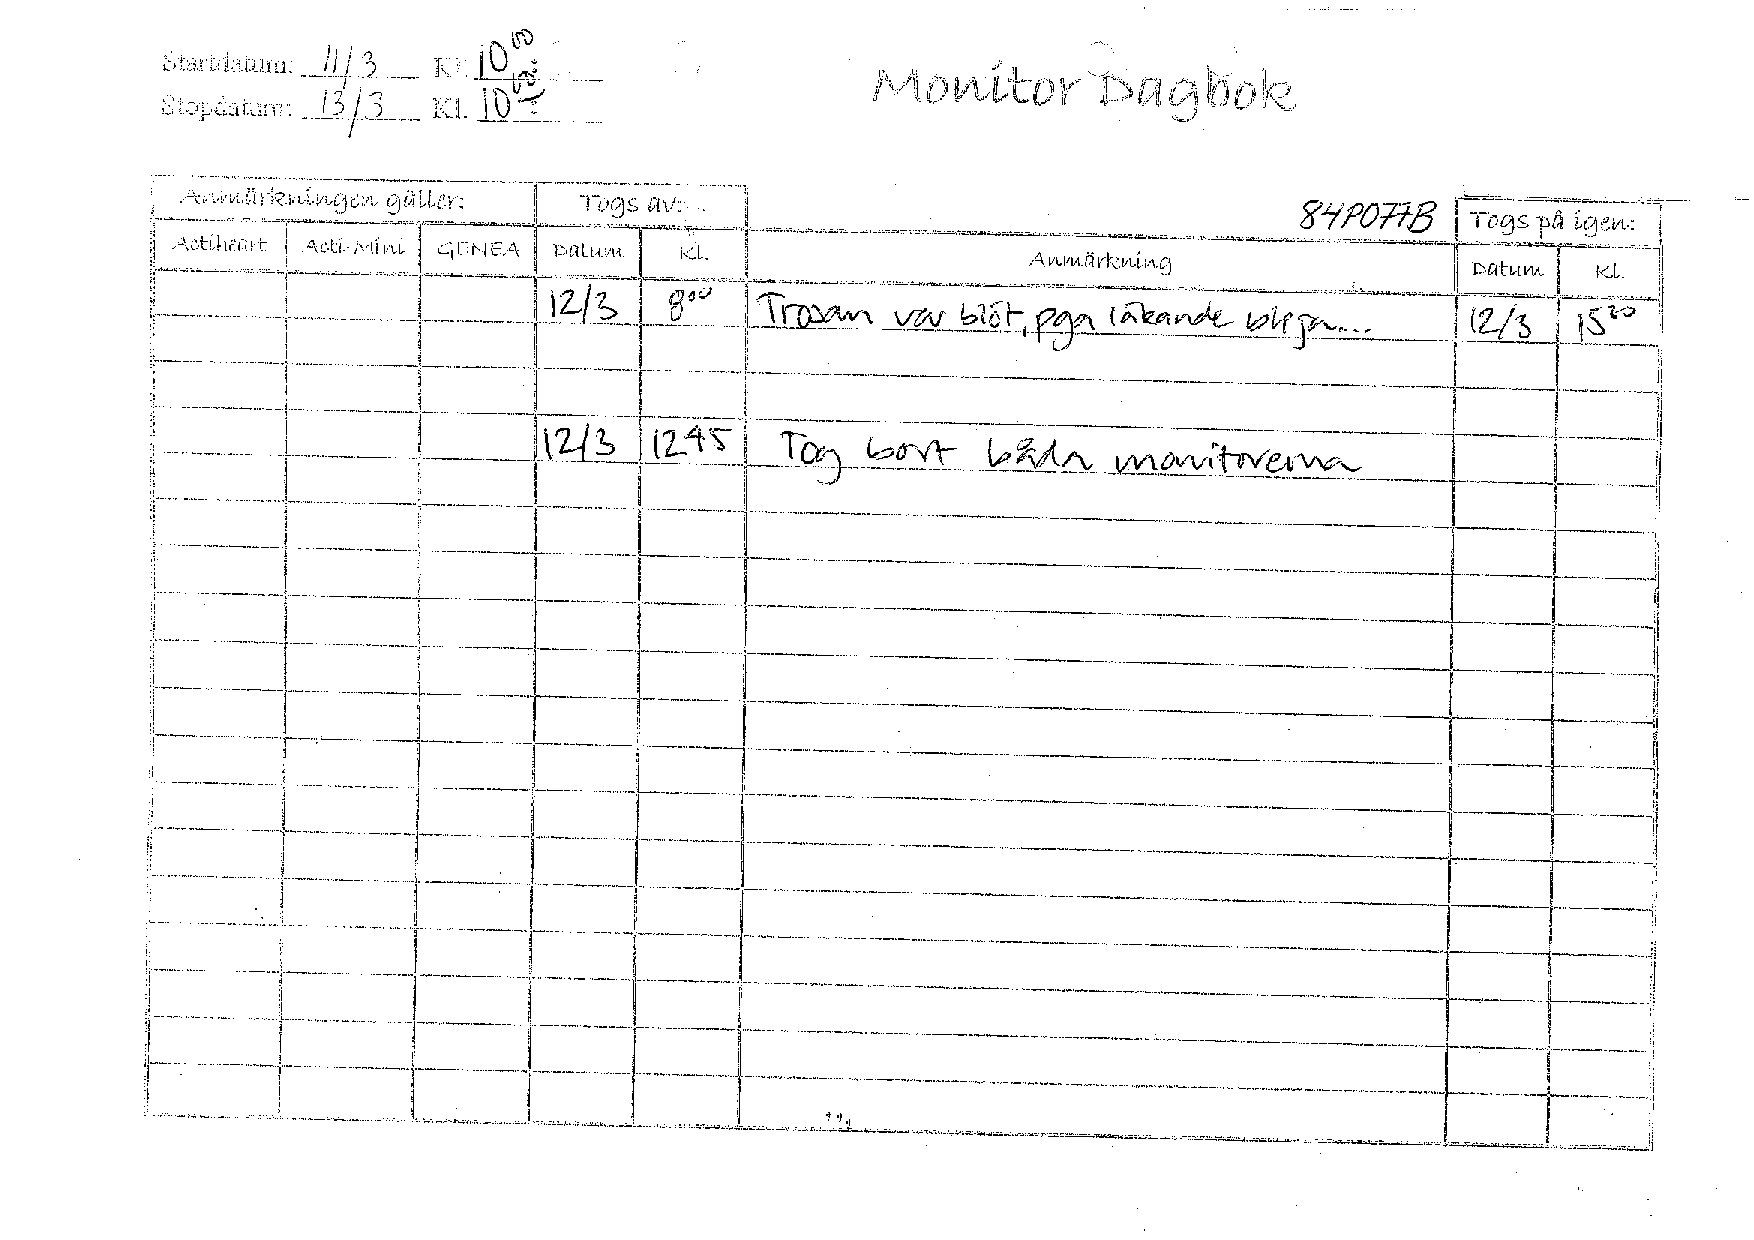
\includepdf[pages=-]{friendly_84P077.pdf}
\end{document}based
